%------------------------------------------------------------------------------%
%%%%%%%%%%%%%%%%%%%%%%%%%%%%%  DISE�O  %%%%%%%%%%%%%%%%%%%%%%%%%%%%%%%%%%%%%%%%%
%------------------------------------------------------------------------------%

\NeedsTeXFormat{LaTeX2e}
\documentclass[12pt]{book}

\usepackage{a4}
\usepackage[Lenny]{fncychap}    % Estilos para capitulos
\usepackage{fancyhdr}           % Estilos para cabeceras
\usepackage[spanish]{babel}
\usepackage[latin1]{inputenc}
\usepackage{epsfig}
\usepackage{subfig}
\usepackage{epstopdf}
\usepackage{caption}
\usepackage{keyval}
\usepackage{graphicx}
\usepackage{float}              % Para poner las imags en cualquier sitio
\usepackage{listings}
\usepackage{color}
\usepackage{textcomp}
\usepackage{verbatim}
\usepackage{exceltex}

\definecolor{listinggray}{gray}{0.98}
\definecolor{lbcolor}{rgb}{0.98,0.98,0.98}
\lstset{
	backgroundcolor=\color{lbcolor},
	tabsize=3,
	rulecolor=,
	language=matlab,
        basicstyle=\footnotesize\sffamily,
        aboveskip={1.5\baselineskip},
        belowskip={1.5\baselineskip},
        columns=fixed,
        showstringspaces=false,
        extendedchars=true,
        breaklines=true,
        prebreak = \raisebox{5ex}[5ex][5ex]{\ensuremath{\hookleftarrow}},
        frame=none,
        showtabs=false,
        showspaces=false,
        showstringspaces=false,
        identifierstyle=\ttfamily,
        keywordstyle=\color[rgb]{0,0,1},
        commentstyle=\color[rgb]{0.133,0.545,0.133},
        stringstyle=\color[rgb]{0.627,0.126,0.941},
}

\usepackage[numbers,sort&compress,comma]{natbib}	% Modo de poner la bibliograf�a
\usepackage{verbatim}      %  \begin{comment}...\end{comment}
\usepackage{subeqnarray}   % equationarray with numbers 1a, 1b, ...
\usepackage{bbm}           % Para s�mbolo tipo n�meros reales. Ej: \bbm{R}
\usepackage{longtable}     % Para tablas largas de m�s de una p�gina
\usepackage{rotating}
\usepackage{psfrag}        % Para cambiar fragmentos de text en .eps por otro en latex
\usepackage{pifont}        % Para otros s�mbolos
\usepackage{fancybox}      % Para encuadrar texto en recuadros
\usepackage{amsmath}       % Mejora la calidad de las formulas
\usepackage{amsfonts}
\usepackage [linktocpage]{hyperref}      % Para enlaces de hipertexto
\usepackage{amssymb,amsfonts}
\usepackage{multirow}
\usepackage{booktabs}
\usepackage{color}
\usepackage{longtable}
\usepackage{float}
\usepackage{array}




\setcounter{tocdepth}{2}             % toc = table of contents. Para definir niveles del �ndice
\setcounter{secnumdepth}{5}          % Hasta cu�ndo se enumeran los caps, seccs, etc


\setlength{\topmargin}{-1.1cm}        % margen por arriba
\setlength{\parskip}{\baselineskip}
\setlength{\parskip}{0.3cm}          % Espacio entre parrafos
\setlength{\textwidth}{16.5cm}       % Ancho del �rea imprimible	
\setlength{\evensidemargin}{-0.4cm}  % Margen izdo en p�ginas pares
\setlength{\oddsidemargin}{0.3cm}    % Margen izdo en p�ginas impares
                                     % evensidemargin = -oddsidemargin !!!

\setlength{\headsep}{1.0cm}
\setlength{\headheight}{3ex}
\setlength{\footnotesep}{5mm}
%\setlength{\mathindent}{1.0cm}       % Controla el espacio entre margen y ec si no est� centrada


%%% Definitionen f�r Fancy Headings
%\renewcommand{\baselinestretch}{3mm}
%\renewcommand{\labelenumi}{\roman{enumi}.}
%\renewcommand{\chaptermark}[1]{\markboth{#1}{}}
%\renewcommand{\sectionmark}[1]{\markright{\thesection\ #1}{}}
\renewcommand{\labelitemi}{$\bullet$}
\renewcommand{\labelitemii}{$\diamond$}
\renewcommand{\labelitemiii}{$\cdot$}

\lhead[\fancyplain{}{\thepage}]{\fancyplain{}{\sl\nouppercase\rightmark}}
\rhead[\fancyplain{}{\sl\nouppercase\leftmark}]{\fancyplain{}{\thepage}}
\cfoot{}
\pagestyle{fancyplain}  		% normale Kopfzeile; ohne Seitenzahl: empty

% Formato de capitulos
\ChTitleVar{\sf\Huge} % Tama�o de la letra del nombre del cap
\ChTitleAsIs


%%% Comando para quitar encabezado y pie de las pag en blanco
\newcommand{\clearemptydoublepage}
  {\newpage{\pagestyle{empty}\cleardoublepage}}

\newcommand{\R}{\mathbb{R}}
\newcommand{\x}{\mathbf{x}}
\newcommand{\grad}{\hspace{-2mm}$\phantom{a}^{\circ}$} %para los grados centigrados

%%% Abstract
\newenvironment{abstract}
  {\begin{center}
   \begin{minipage}{0.8\textwidth}
   \slshape}
  {\end{minipage}
   \end{center}}


\typeout{ }
\typeout{----------------------------------------------------------------------}
\typeout{ }



%------------------------------------------------------------------------------%
%%%%%%%%%%%%%%%%%%%%%%%%%%%%%%  DOCUMENTO  %%%%%%%%%%%%%%%%%%%%%%%%%%%%%%%%%%%%%
%------------------------------------------------------------------------------%


\begin{document}


\renewcommand{\listfigurename}{�ndice de figuras}
\renewcommand{\listtablename}{�ndice de tablas}
\renewcommand{\bibname}{Bibliograf�a}
\renewcommand{\contentsname}{�ndice}
\renewcommand{\figurename}{Figura}
\renewcommand{\tablename}{Tabla}
\renewcommand{\partname}{Parte}
\renewcommand{\chaptername}{Cap�tulo}
\renewcommand{\appendixname}{Ap�ndice}

  \pagenumbering{roman}    % Numeraci�n de p�ginas con num romanos
  \setcounter{page}{1}      % Establece la siguiente p�gina como la 1
	\begin{titlepage}
\label{ch:portada}
\begin{center}

{\Large\textsc{Ingenier�a de Telecomunicaci�n}}


Departamentos:  \\ Arquitectura y Tecnolog�a de Computadores \\ Teor�a de la Se�al, Telem�tica y Comunicaciones

\textbf{Universidad de Granada}


\vspace{0.5cm}

\begin{figure}[h]
	\centering
	\epsfig{file=figuras/Portada/portada1, width=7cm}
	\label{fig:ugr}
\end{figure}


\vspace{0.5cm}
\textbf{PROYECTO FIN DE CARRERA}


\vspace{0.9cm}


{\Huge\textbf{Desarrollo de una aplicaci�n de visualizaci�n de datos y configuraci�n para sistemas de monitorizaci�n y an�lisis del movimiento del cuerpo humano.}}


\end{center}


\vspace{1.5cm}
\textbf{Realizado por:}  \hfill \textbf{Dirigido por:}

Javier L�pez Garc�a \hfill D. Alberto Olivares Vicente

\hfill D. Gonzalo Olivares Ruiz

\end{titlepage}
						% Inclu�mos la portada en espa�ol
  \clearemptydoublepage
  
%Abstract
%--------

\begin{titlepage}
\label{ch:RAbstract}
\vspace{3cm}

\noindent \textbf{Desarrollo de una aplicaci�n de visualizaci�n de datos y configuraci�n para sistemas de monitorizaci�n y an�lisis del movimiento del cuerpo humano}

\vspace{1cm}
\noindent \large PALABRAS CLAVE:

\noindent Sensores inerciales, IMU, MEMS, aceler�metros, gir�scopos, magnet�metros, calibraci�n, c�lculo de la orientaci�n, GaitWatch, ECnsole, Matlab, GUI.

\vspace{1cm}
\noindent \large RESUMEN:

\noindent
Este proyecto se centra en desarrollar una aplicaci�n gr�fica en Matlab que permita la configuraci�n y visualizaci�n de los datos recogidos por los sistemas de medida de par�metros de la marcha GaitWatch Manager y ECnsole. Los objetivos principales son: elaborar un an�lisis de los sistemas de monitorizaci�n de la marcha existentes en la actualidad que presentan caracter�sticas similares; desarrollar un software espec�fico que reuna los requisitos necesarios establecidos inicialmente (visualizar y configurar los datos extraidos de los sistemas citados anteriormente); e integrar los algoritmos de calibraci�n y c�lculo de la orientaci�n calculando las se�ales requeridas de forma imperceptible para el usuario de la aplicaci�n.

\end{titlepage} 
  \clearemptydoublepage
  
%Declaraci�n
%--------

\begin{titlepage}
\label{ch:RDeclaracion}
\vspace{2cm}

\noindent D. Gonzalo Olivares Ruiz profesor del departamento de Arquitectura y Tecnolog�a de los Computadores de la Universidad de Granada, y D. Alberto Olivares Vicente, profesor  del dpto. de Teor�a de la Se�al, Telem�tica y Comunicaciones,  como directores del Proyecto Fin de Carrera de D. Javier L�pez Garc�a,

\vspace{2cm}
\noindent Informan:

\vspace{1.5cm}
\noindent Que el presente trabajo, titulado:

\noindent \textbf{Desarrollo de una aplicaci�n de visualizaci�n de datos y configuraci�n para sistemas de monitorizaci�n y an�lisis del movimiento del cuerpo humano.}

\noindent Ha sido realizado y redactado por el mencionado alumno bajo nuestra direcci�n, y con esta fecha autorizamos a su presentaci�n.
\vspace{3.5cm}

\noindent Granada, a XX de Septiembre de 2014 Fdo:

\vspace{6.5cm}
\noindent D. Alberto Olivares Vicente  \hfill D. Gonzalo Olivares Ruiz

\end{titlepage} 
  \clearemptydoublepage
  
%Agradecimientos
%---------------


\begin{titlepage}
\label{ch:Agradecimientos}
\vspace{3cm}

\noindent {\Large\textbf{Agradecimientos}}
\vspace{0.5cm}

En primer lugar me gustar�a darle las gracias al departamento de Arquitectura y Tecnolog�a de computadores y al departamento  Teor�a de la Se�al, Telem�tica y Comunicaciones por darme la posibilidad de realizar este proyecto.

Adem�s quisera agradecer a mis tutores Gonzalo Olivares y Alberto Olivares su inestimable ayuda y dedicaci�n. Sin su ayuda no hubiera sido posible.


Darle las gracias tambi�n a mi familia que durante estos a�os me ha dado la oportunidad de formarme adecuadamente y llegar a conseguir los objetivos que me hab�a fijado.
\end{titlepage}



	%Inclu�mos los agradecimientos
  \addcontentsline{toc}{chapter}{Agradecimientos}	
  \tableofcontents          % Pone �ndice
  \clearemptydoublepage
  \listoffigures						% Crea la lista de figuras
	\listoftables							% Crea la lista de tablas
  \pagenumbering{arabic}    % Numeraci�n de p�ginas con num normales (�rabes)
  %%% Capitulos
\clearemptydoublepage

\chapter{Introducci\'on}
\label{ch:Introduccion}

\section{Estado del arte}

En este punto comenzaremos estudiando algunos dispositivos existentes en la actualidad y que son utilizados para la monitorización del cuerpo humano así como las prestaciones de cada uno de ellos.

Posteriormente se realizará un sondeo de los métodos y procedimientos adoptados en diferentes estudios para el análisis de los ajustes posturales anticipatorios en diferentes casos, así como las aplicaciones de los mismos.

Finalmente, hablaremos de las técnicas más comunes de calibración, preprocesado y clasificación.

\subsection{Instrumentaci\'on}

Existen varios tipos de dispositivos usados para la medida de los APAs, destacando: el electromiógrafo, las plataformas de fuerza, los sensores inerciales y dispositivos basados en cámaras.

La electromiografía (EMG) es una técnica que nos da información sobre la actividad eléctrica de los músculos del esqueleto (Ver figura [1]). El electromiógrafo es capaz de detectar la actividad eléctrica debido a una diferencia de potencial en las células musculares, siendo muy útil, además de para el análisis de posturas corporales,  para localizar lesiones como parálisis musculares y el lugar donde éstas se producen \cite{Marcio2010} \cite{Instr1}. 


Hasta el momento, la gran mayoría de los estudios realizados han incluido como dispositivo de medida, entre otros,  una plataforma sensible a la fuerza y la presión.  Sin embargo, el coste y la complejidad de medir los APAs con un análisis del movimiento tradicional, usando plataformas de fuerza y sistemas EMG limita sus aplicaciones en la práctica clínica. Por ello, recientemente se ha optado por sensores inerciales pequeños, baratos y portables. Aun así, en nuestro caso, se ha utilizado dicha plataforma, contemplando la posibilidad de prescindir de ella en un futuro \cite{Mancini2009} \cite{Vennila2011}.

Los dispositivos fundamentados en sensores inerciales comúnmente utilizados son las IMU (inertial measurement unit) , un dispositivo electrónico que mide e informa acerca de la velocidad, orientación y fuerzas gravitacionales de un aparato, usando una combinación de acelerómetros y giróscopos.
 También existe la posibilidad de combinarlos con magnetrómetros, pasándose a llamar MIMO. Algunos de los dispositivos MIMO existentes actualmente en el mercado son: 3DN-GX4-45 \cite{Instr2},  xsens-mvn \cite{Instr3} y mvn-biomech \cite{Instr4}, donde todos ellos utilizan sensores de tipo Microelectromecánico (MEMS).
 
 \begin{figure}[H]
 	\centering
 	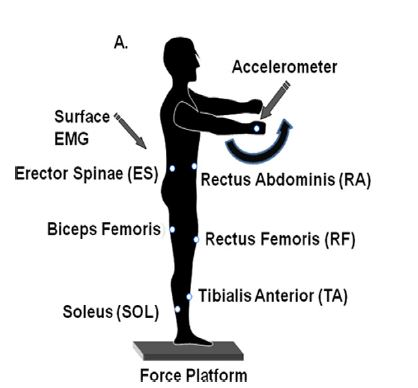
\epsfig{file=imagenes/Captura, width=7cm}
 	\caption{EMG, acelerómetros y plataforma \cite{Gay2011}.}
 	\label{fig:arte1}
 \end{figure}
 
Existen marcadores de reflexión infrarroja que nos da una medida más compleja de la postura. Estos se reparten por el cuerpo y nos pueden proporcionar información sobre estrategias posturales, lo que nos permite saber si el balanceo del cuerpo se realiza teniendo como punto central de oscilación el tobillo o se debe movimiento de cadera, por ejemplo . En la figura [2]se muestra la disposición del sistema.

\begin{figure}[H]
	\centering
	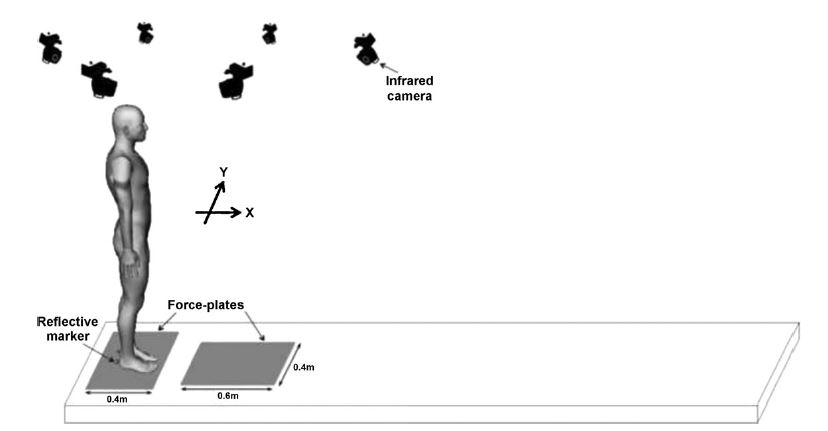
\epsfig{file=imagenes/Captura2, width=7cm}
	\caption{Esquema con mascadores de reflexión infrarroja \cite{Teddy2013}.}
	\label{fig:arte2}
\end{figure}

Como se ha mencionado anteriormente, también existe la posibilidad de utilizar sensores basados en cámaras que generalmente forman parte de sistemas ópticos de captura del movimiento humano, tales como Kinect \cite{Instr5}.


\subsection{M\'etodos y procedimientos}

Hasta el momento se ha realizado numerosos estudios acerca de los Ajustes Posturales Anticipatorios, principalmente en los últimos seis años. 
La finalidad de la mayoría de estas investigaciones es poder profundizar en el conocimiento de qué es lo que realmente ocurre cuando iniciamos un determinado movimiento, si este hecho sigue un determinado patrón y de las condiciones de las que depende.

Si analizamos el estado del arte de los APAs podemos encontrar que las primeras investigaciones intentaban confirmar la hipótesis de si los APAs estaban asociados a un movimiento voluntarios, confirmándose así la hipótesis y llegando a la conclusión de que es más probable que los ajustes no aparezcan cuando el inicio el movimiento no está planeado, es decir, cuando es evocado por una perturbación. Esto es esencial en el control del balance en el momento de andar ya que el conocimiento de esto se podría utilizar para prevenir caídas en personas con dificultades de movilidad, por ejemplo.\cite{Mcllroy1993}\cite{Yiou2012}\cite{Teddy2013}\cite{Bouisset2008}\cite{Neeta2014}

Posteriormente se han ido comprobando la influencia de otro tipo de variables, como la realización de ejercicios diversos donde se estimulan músculos diferentes y la reacción de dichos músculos\cite{Gay2011}; la influencia de la edad para generar patrones posturales \cite{Bleuse2006} \cite{Estelle2008}; el tipo de señal que inicia el movimiento (visual o auditiva) ya que influye en la reacción del cuerpo ante dicha estimulación \cite{Mcllroy1993}\cite{Antonia2009}\cite{Vicent1999}\cite{Tard2013}; como el miedo a caerse afecta a la postura que se adopta al iniciar a andar[26] o como enfermedades neurodegenerativas, como Parkinson o la Esclerosis múltiple\cite{Mancini2009}\cite{Jebb2008}\cite{Chris2005}\cite{Hall2013}, o parálisis cerebrales, tales como hemiplegia o diplegia\cite{Hall2013}, generan diferencias en los APAs.

Todos estos estudios tienen una gran importancia en aplicaciones médicas. Por ejemplo, tal y como se ha dicho anteriormente, hay enfermedades que afectan al sistema nervioso central y por tanto, a la movilidad, provocando en muchas ocasiones caídas lo que implica que estas personas que las sufren padezcan miedo a volver a caer de nuevo. El hecho de confirmar que el propio miedo a la caída provoca variaciones en los APAs haciendo que estas personas sean más propensas a nuevas caídas nos podría ayudar a prevenirlas.

\subsection{An\'alisis de datos}

En los últimos años se han realizado numerosos trabajos relacionados con la calibración de acelerómetros y giróscopos, aunque la mayoría muestran pequeñas variaciones con respecto a otros estudios realizados anteriormente. Uno de los trabajos más destacados \cite{Kian2011}muestra una forma de realizar la calibración colocando los acelerómetros en seis posiciones diferentes y aplicando algoritmos algebraicos sencillos a los datos obtenidos. El giróscopo de calibra de forma distinta, mediante una proceso basado en una rotación conocida. A parte de este método anterior, existen otros basado al igual que él en la colocación de los acelerómetros en seis posiciones.

Existen otros métodos que intentan ser más precisos, aumentando el número de posiciones en las que se realiza la recogida de datos \cite{Camps2009}. También existen otro tipo de técnicas de calibración como algoritmos basados en operaciones algebraicas básicas o basados en filtros FIR. \cite{A.Olivares2013}

En cuanto a la estimación de la orientación para la monotorización del cuerpo humano, si se realiza un estudio de los trabajos existentes hasta el momento se puede ver que casi todos ellos se basan en la utilización del filtro de Kalman, sin embargo el resultado con señales de baja intensidad no suele ser muy preciso.\cite{A.Olivares2013}

Finalmente, analizamos el estado del arte del reconocimiento de movimientos en humanos y clasificadores. Rápidamente se puede ver que la cantidad de información relativa al campo de la clasificación en bastante grande, existiendo numerosos artículos y libros con información acerca de ello. Sin embargo, existen otro tipo de estudios, como en el que nos centraremos \cite{Banos2012}, donde se exponen métodos para el reconocimiento de actividad humana basados en un clasificador jerárquico ponderado. En él se indican diferentes esquemas de clasificación que podrían ser usados y que mejores resultados proporcionan para reconocer secuencias de actividad, tales como andar o correr.



\clearemptydoublepage
\chapter{Monitorizaci\'on del cuerpo humano}
\label{ch:monitorizacion}

\section{Definici�n y �mbito de uso}


GaitWatch  y ECnsole son sistemas para la monitorizaci�n y an�lisis de los par�metros de la marcha. Inicialmente vamos a definir el concepto, la historia y los par�metros que caracterizan la marcha humana. Para situarnos mejor y poner en contexto los sistemas utilizados, debemos incluir estos dispositivos dentro de los  sistemas de captura del movimiento. El concepto es m�s amplio y engloba un mayor n�mero de aplicaciones. La captura de movimiento es el proceso de registrar el movimiento de objetos o personas, es decir, no s�lo bajo condiciones de desplazamiento. En los apartados siguiente se describir�n varias de las aplicaciones y la forma de clasificar los sitemas de captura del movimiento presentes en la actualidad.

\subsection{Definici�n: An�lisis de la marcha}


La marcha humana \cite{moni1} es un proceso de locomoci�n en el que el cuerpo humano, en posici�n erguida, se mueve hacia delante, siendo su peso soportado alternativamente por ambas piernas. Mientras el cuerpo se desplaza sobre la pierna de soporte, la otra pierna se balancea hacia delante como preparci�n para el siguiente apoyo.


La ciencia encargada del an�lisis de la marcha es la biomec�nica \cite{moni2}. En la actualidad contin�a en desarrollo debido a la dificultad para conseguir 
establecer una normalizaci�n. Una misma persona puede realizar el mismo movimiento de 
formas muy distintas, ya que influyen m�ltiples factores como la carga exterior a�adida, la 
velocidad y, en el caso del caminar, tambi�n el calzado. Adem�s, cada movimiento 
humano, realizado por las extremidades superiores o inferiores, depende en gran medida de 
las dimensiones de las mismas y de la distribuci�n de la masa, con lo que el mismo 
movimiento puede diferir mucho de una persona a otra. El hecho de que no exista el 
\textit{hombre medio} complica este tipo de estudios. Las dimensiones del cuerpo humano var�an 
seg�n edad, sexo, raza, e incluso grupo laboral. 


\subsection{Historia}

Los pioneros de la investigaci�n cient�fica sobre el an�lisis de la marcha fueron Arist�teles en De Motu Animalium (En la marcha de los Animales) y m�s tarde en 1680, Giovanni Alfonso Borelli, tambi�n llamado De Motu Animalium (I et II). En la d�cada de 1890, el anatomista alem�n Christian Wilhelm Braune y Otto Fischer public� una serie de documentos sobre la biomec�nica de la marcha humana en condiciones de carga y descarga.

Con el desarrollo de la fotograf�a, se hizo posible la captura de secuencias de im�genes que revelan detalles de la locomoci�n humana y animal que pueden ser percibidos con el ojo humano. Eadweard Muybridge y Marey �tienne-Jules fueron los pioneros de esta pr�ctica a principios de 1900. Por ejemplo, fue la fotograf�a la que revel� por primera vez la secuencia detallada de la marcha del caballo ''a galope" , que sol�a estar mal representada en las pinturas realizadas con anterioridad a este descubrimiento.

Aunque las investigaciones anteriores fueron hechas en el campo de las c�maras de pel�cula, la aplicaci�n generalizada de an�lisis de la marcha se realiza en seres humanos que presentan patolog�as como par�lisis cerebral, enfermedad de Parkinson y trastornos neuromusculares, que se inici� en la d�cada de los 70 con la ayuda de sistemas de c�mara de v�deo que pueden realizar los estudios detallados de cada uno de los pacientes dentro de los l�mites realistas de costes y tiempo. El desarrollo de reg�menes de tratamiento, a menudo en cirug�a ortop�dica, basados en los resultados de an�lisis de la marcha han avanz� significativamente en la d�cada de los 80. Muchos de los principales hospitales ortop�dicos en todo el mundo tienen ahora los laboratorios para realizar estos estudios de la marcha que se utilizan habitualmente en un gran n�mero de casos m�dicos, tanto para el dise�o de planes de tratamiento como para el control de seguimiento.



La implementaci�n de ordenadores modernos con la tecnolog�a para realizar estos estudios se produjo de forma independiente a finales de la d�cada de de los 70 y principios de los 80 en laboratorios de investigaci�n de varios hospitales, algunos a trav�s de colaboraciones con la industria aeroespacial. Pronto sigui� con el desarrollo comercial, con la aparici�n de sistemas de movimiento Vicon y BTS, y con el marketing de sistemas de an�lisis de la marcha a mediados de la d�cada de 1980.

Para m�s informaci�n sobre la historia del estudio de la marcha consulte  \cite{moni3}.

\subsection{F�ctores y par�metros}


El proceso de deambulaci�n est� modulado o modificado por muchos factores \cite{moni3}, y los cambios que imprimen en el patr�n de marcha habitual pueden ser transitorios o permanentes. Los factores pueden ser de diversos tipos:

\begin{itemize}
\item \textbf{Extr�nsecos}: Hay varios factores extr�nsecos, como por ejemplo el terreno, el calzado, la vestimenta, transporte de carga.

\item \textbf{Intr�nsecos}: Los factores intr�nsecos son sexo (hombre y mujer), peso, altura, edad,etc.

\item \textbf{F�sicos}: Los factores f�sicos incluyen el peso, la talla y la constituci�n f�sica.

\item \textbf{Psicol�gicos}: Los factores psicol�gicos incluyen la personalidad y las emociones.

\item \textbf{Fisiol�gicos}: Cuando se habla de factores fisiol�gicos se trata de caracter�sticas antropom�tricas.

\item \textbf{Patol�gicos}: Los factores patol�gicos pueden ser por ejemplo traumatismos, patolog�as neurol�gicas, m�sculo esquel�tica y trastornos psiqui�tricos.

\end{itemize}




Los par�metros \cite{moni1} que se tiene en cuenta para el an�lisis de la marcha son:

\begin{itemize}
\item \textbf{Longitud del paso completo}: Es la distancia lineal entre los sucesivos puntos de contacto del tal�n de mismo pie. Aproximadamente 156 cm por paso completo.

\item \textbf{Longitud del paso}: Es la distancia lineal en el plano de progresi�n entre los puntos de contacto de un pie y el otro pie. La mitad en cm de la longitud de paso completo. Estos 2 par�metros se pueden ver en la figura \ref{fig:moni1}:

\begin{figure}[H]
\centering
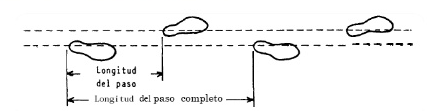
\includegraphics[width=0.7\textwidth]{figuras/monitorizacion/moni1}

\caption{Longitud de paso y de zancada \cite{moni1}.}
\label{fig:moni1}
\end{figure}

\item \textbf{Cadencia}: El n�mero de pasos por unidad de tiempo (pasos por minuto). Aproximadamente entre 60 y 117 pasos por minuto.
\item \textbf{Anchura del paso}: La distancia entre la l�nea media de un pie y l�nea media del otro pie. De 5 a 10 cm. Se muestra en la figura \ref{fig:moni2}:

\begin{figure}[H]
\centering
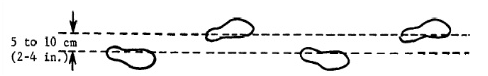
\includegraphics[width=0.7\textwidth]{figuras/monitorizacion/moni2}

\caption{Anchura del paso \cite{moni1}.}
\label{fig:moni2}
\end{figure}


\item \textbf{Angulo del pie}: El �ngulo en el cual normalmente se desv�a la punta del pie hacia fuera de la l�nea de progresi�n. De 6.7 a 6.8 grados. Se muestra en la figura \ref{fig:moni3}:

\begin{figure}[H]
\centering
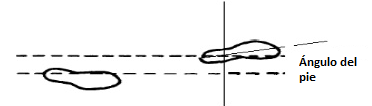
\includegraphics[width=0.7\textwidth]{figuras/monitorizacion/moni3}

\caption{�ngulo del pie \cite{moni1}.}
\label{fig:moni3}
\end{figure}



\end{itemize}


\subsection{Aplicaciones de los sistemas de captura del movimiento humano}

Los sistemas HMC (c�ptura del movimiento humano) tienen un gran n�mero de aplicaciones \cite{moni4}, que se han visto significativamente incrementado en los �ltimos a�os. Entre estas aplicaciones se pueden destacar las siguientes:


\begin{itemize}

\item \textbf{Animaci�n de personajes virtuales en el cine:} En el cine se emplean cada vez m�s personajes generados por ordenador. Para conseguir que dichos personajes act�en y se muevan de forma natural, se capturan los movimientos de un actor real y luego dichos movimientos se trasladan al cuerpo del actor virtual. En la figura \ref{fig:moni4} tenemos un ejemplo.

\begin{figure}[H]
\centering
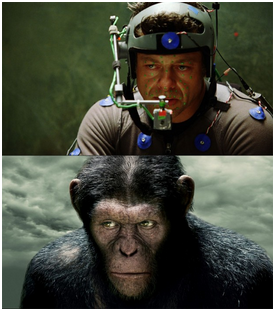
\includegraphics[width=0.4\textwidth]{figuras/monitorizacion/moni4}

\caption{Im�genes de la producci�n \textit{El origen del planeta de los simios} \cite{moni4}.}
\label{fig:moni4}
\end{figure}

\item \textbf{Animaci�n de personajes virtuales en videojuegos}: Los videojuegos (de ordenador y de consola) son hoy d�a la principal industria del ocio. Su complejidad y grado de realismo ha aumentado enormemente en los �ltimos a�os. Al igual que ocurre en el cine, para conseguir personajes que se mueven de forma fluida y natural, se capturan los movimientos de un actor real y luego se trasladan al actor virtual. La figura \ref{fig:moni5} muestra el proceso.

 Los sistemas HMC empleados para capturar movimientos para el cine o para un videojuego son esencialmente los mismos y, aunque tradicionalmente en los videojuegos se permit�an animaciones de calidad algo inferior, la brecha entre ambas aplicaciones se va cerrando conforme los videojuegos crecen en complejidad, detalle y rentabilidad.

\begin{figure}[H]
\centering
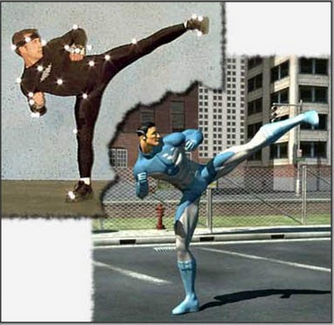
\includegraphics[width=0.4\textwidth]{figuras/monitorizacion/moni5}

\caption{Animaci�n de personajes virtuales en videojuegos \cite{moni4}.}
\label{fig:moni5}
\end{figure}

\item \textbf{Aplicaciones m�dicas}: Los sistemas HMC como el mostrado en la figura \ref{fig:moni7} se utilizan con fines m�dicos, para detectar lesiones, malformaciones o problemas a partir del an�lisis de los movimientos de una persona, para recopilar datos sobre la evaluaci�n del paciente en terapias de rehabilitaci�n, o para realizar estudios de ergonom�a (por ejemplo, comprobar si un determinado mobiliario de oficina fuerza posturas perjudiciales o no).

\begin{figure}[H]
\centering
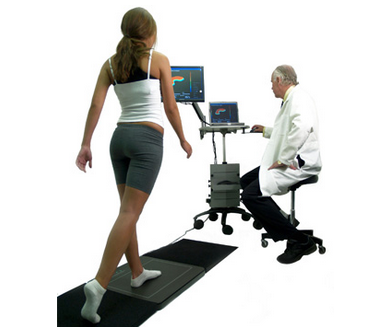
\includegraphics[width=0.35\textwidth]{figuras/monitorizacion/moni6}
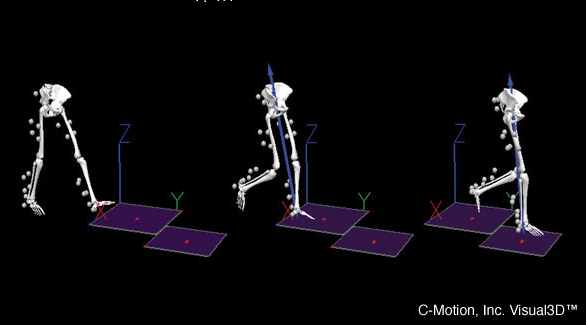
\includegraphics[width=0.35\textwidth]{figuras/monitorizacion/moni7}

\caption{Aplicaciones m�dicas \cite{moni4}.}
\label{fig:moni7}
\end{figure}



\item \textbf{Interfaces humano-m�quina avanzados}: El control de un ordenador mediante gestos puede realizarse si se utiliza un sistema HMC que capture los movimientos de una persona, sobre todo los de las manos, y en la cara los ojos para saber d�nde est� mirando. Como el de la figura \ref{fig:moni9}.

\begin{figure}[H]
\centering
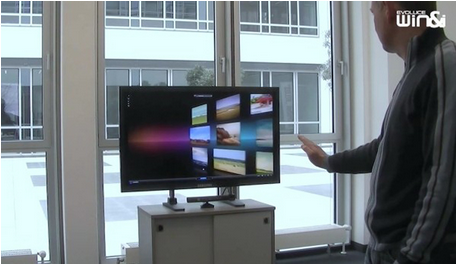
\includegraphics[width=0.35\textwidth]{figuras/monitorizacion/moni8}
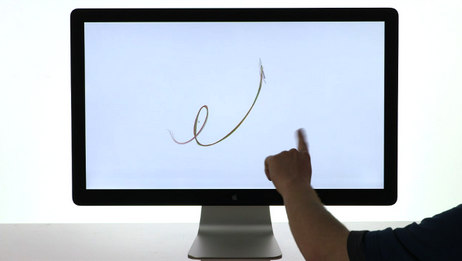
\includegraphics[width=0.35\textwidth]{figuras/monitorizacion/moni9}

\caption{Interfaces humano-m�quina avanzados \cite{moni4}.}
\label{fig:moni9}
\end{figure}

\item \textbf{Sistemas de vigilancia}: Un sistema de seguridad que vigile una determinada zona (por ejemplo, una c�mara de vigilancia en un parking) puede ver su eficacia multiplicada si se le a�aden funcionalidades de captura y an�lisis de movimiento autom�ticos. La figura \ref{fig:moni10} muestra este tipo de sistema. Observando el patr�n de movimientos de una persona, por ejemplo, se pueden detectar conductas sospechosas (por ejemplo, una persona en un parking que en lugar de entrar o salir de un coche da vueltas en torno a ellos, examin�ndolos) o situaciones potencialmente peligrosas (por ejemplo, una persona que deja una mochila en un rinc�n y se marcha).

\begin{figure}[H]
\centering
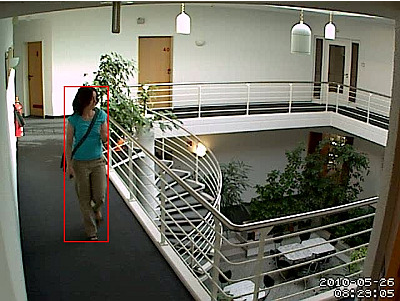
\includegraphics[width=0.35\textwidth]{figuras/monitorizacion/moni10}
\caption{Sistema de vigilancia \cite{moni4}.}
\label{fig:moni10}
\end{figure}

\item \textbf{Sistemas de interacci�n y aprendizaje para robots sociales}: Un robot social debe cooperar con personas en tareas cotidianas. Eso implica ser capaz de percibir a la persona y analizar sus movimientos, con un sistema HMC, para coordinar la acci�n del robot con esos movimientos. La figura \ref{fig:moni11} nos muestra un ejemplo.

\begin{figure}[H]
\centering
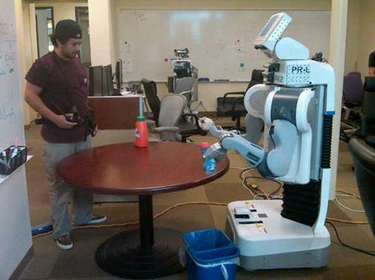
\includegraphics[width=0.35\textwidth]{figuras/monitorizacion/moni11}
\caption{Sistema de interacci�n y aprendizaje para para un robot \cite{moni4}.}
\label{fig:moni11}
\end{figure}

\end{itemize}


\subsection{Clasificaci�n de los sistemas de captura del movimiento humano}


Hay muchas formas distintas de capturar los movimientos de una persona. Los sistemas de captura var�an en su precio, precisi�n, complejidad, tiempo de respuesta, robustez, versatilidad, etc.  



En la figura \ref{fig:moni12} se pueden distinguir dos bloques principales en funci�n del tipo de tecnolog�a utilizada: los sistemas fundamentados en c�maras  y los que no. Cuando lleguemos al apartado del \textit{Estado del Arte} nos centraremos exclusivamente en los sistemas que funcionan con sensores inerciales (los dispositivo GaitWatch y ECnsole pertenecen a este grupo) y de manera m�s gen�rica se tratar�n los distintos tipos de dispositivos de captura del movimiento con c�maras.


\begin{figure}[H]
\centering
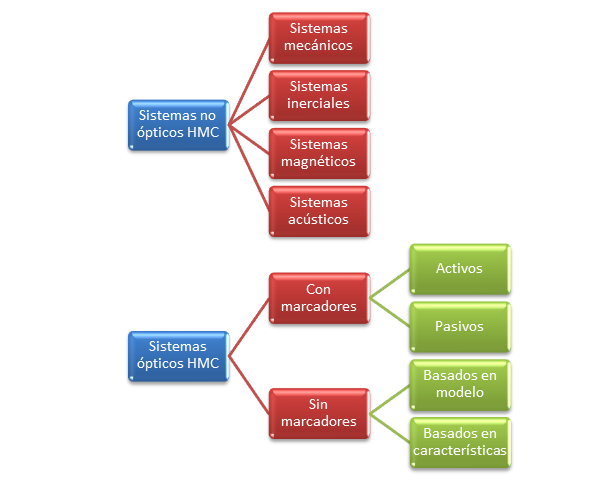
\includegraphics[width=0.6\textwidth]{figuras/monitorizacion/moni12}
\caption{Clasificaci�n de sistemas de captura del movimiento}
\label{fig:moni12}
\end{figure}

Toda la informaci�n acerca de la clasificaci�n de los sistemas HMC ha sido extraida en \cite{moni5} donde se hace una clasificaci�n minuciosa de este tipo de sistemas.
\subsubsection{Sistemas de captura del movimiento no �pticos}


Los sistemas HMC no �pticos se dividen en las siguientes categor�as:

\vspace{1cm}

\textbf{Sistemas mec�nicos}:

Consisten en una serie de brazos mec�nicos como los que se muestran en la figura \ref{fig:moni13}, adheridos mediante alg�n sistema de agarre o anclaje a diversas partes del cuerpo del usuario (por ejemplo, un cierre sobre la mu�eca del mismo), de forma que dichos brazos sigan los movimientos de las extremidades, torso, cabeza, etc., del usuario. Los �ngulos de giro de estos brazos mec�nicos (que conforman lo que se conoce como exoesqueleto) se corresponden con los �ngulos de giro de las articulaciones.


\begin{itemize}
\item Ventajas
	\begin{itemize}
	\item Se obtiene informaci�n muy precisa.
	\item Son muy r�pidos.
	\item Son muy robustos frente a distorsiones producidas, por ejemplo, por el temblor de la mano.
	\item Son inmunes a interferencias y oclusiones.
	\end{itemize}
\end{itemize}


\begin{itemize}
\item Inconvenientes
	\begin{itemize}
	\item Es necesario otro sistema de seguimiento para efectuar medidas de posici�n.
	\item El montaje de estos sistemas es muy aparatoso.
	\item Las propias limitaciones del movimiento mec�nico y la necesidad de mantener fijos los puntos de uni�n al cuerpo del usuario disminuyen considerablemente los grados de libertad que el sistema de seguimiento es capaz de registrar, adem�s de afectar a la movilidad del propio usuario.
	\item Debido a que s�lo registran �ngulos de giro, tienden a generar movimientos poco naturales, en los que el modelo de persona parece una marioneta que cuelga de hilos.
	\end{itemize}
\end{itemize}








\begin{figure}[H]
\centering
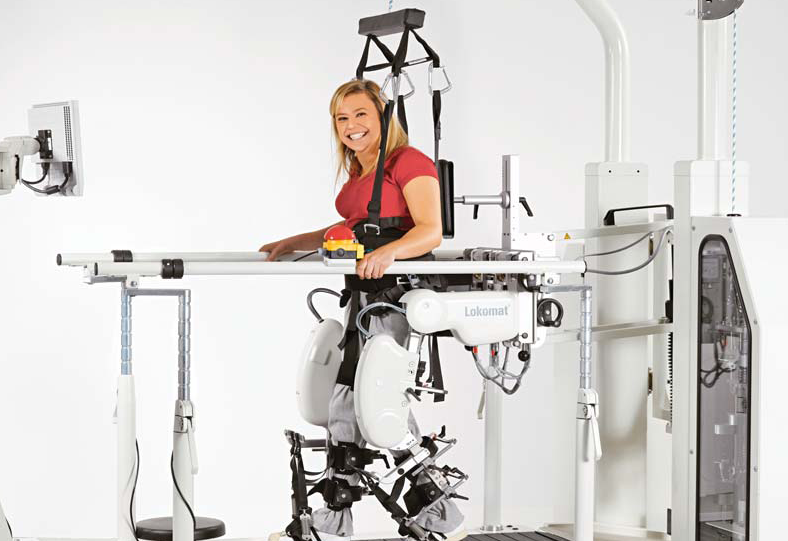
\includegraphics[width=0.4\textwidth]{figuras/monitorizacion/moni13}
\caption{Exoesqueleto con monitorizaci�n de movimientos \textit{Lokomat} \cite{moni5}.}
\label{fig:moni13}
\end{figure}

\textbf{Sistemas inerciales}:

Estos sistemas se basan en el empleo de sensores inerciales en miniatura, usualmente gir�scopos que miden la rotaci�n de cada articulaci�n (una tecnolog�a similar a la usada en el mando de la Wii). Mediante estos dispositivos, por el principio de conservaci�n del momento angular, se pueden calcular los giros en los ejes longitudinal, transversal y vertical partiendo de la resistencia inercial presentada por el giroscopio a un cambio en su orientaci�n. Los valores de estos �ngulos se env�an usualmente a trav�s de un enlace wireless a un ordenador donde los datos se filtran y procesan para conformar la pose percibida.


\begin{figure}[H]
\centering
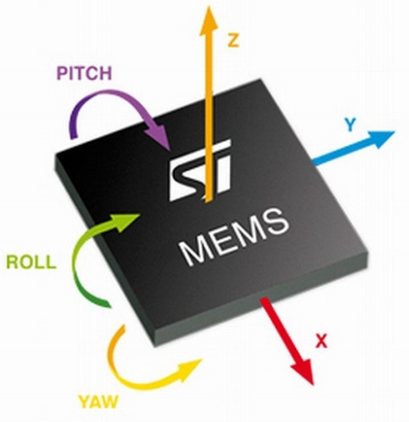
\includegraphics[width=0.32\textwidth]{figuras/monitorizacion/moni26}

\caption{Sistema inercial. �ngulos de orientaci�n \cite{moni13}.}
\label{fig:moni26}
\end{figure}

\begin{itemize}
	\item Ventajas
	\begin{itemize}
	\item Tienen un alcance muy amplio, por lo que su rango de acci�n es considerablemente elevado.
	\item No necesitan de un entorno controlado para ser utilizados.
	
	\end{itemize}
	\item Incovenientes
	\begin{itemize}
		\item Es necesario otro sistema de seguimiento para efectuar medidas de posici�n.
		\item Mucha sensibilidad a las vibraciones.
		\item Tendencia a presentar derivas provocadas por acumulaci�n de errores.
		
	\end{itemize}
\end{itemize}



\textbf{Sistemas magn�ticos}:

Estos sistemas (vease figura \ref{fig:moni15}) utilizan un dispositivo transmisor de pulsos y una serie de receptores. Su principio de funcionamiento consiste en generar en el transmisor tres campos electromagn�ticos perpendiculares, y cada receptor calcula la atenuaci�n producida en cada campo. Con esta informaci�n, se calcula la posici�n y la orientaci�n del receptor mediante una triangulaci�n de los datos recibidos en relaci�n a los tres ejes correspondientes a los campos electromagn�ticos generados inicialmente.

\begin{itemize}
	\item Ventajas
	\begin{itemize}
	\item Proporcionan informaci�n sobre los 6 grados de libertad de las articulaciones usando menos sensores que otros sistemas (por ejemplo, s�lo dos tercios de la cantidad que requerir�a un sistema HMC �ptico que proporcionase la misma informaci�n).
	\item No se ven afectados por oclusiones de objetos no met�licos.
	
	\end{itemize}
	\item Incovenientes
	\begin{itemize}
		\item El cableado de los sensores hace a estos sistemas aparatosos y molestos a la hora de realizar movimientos amplios y/o r�pidos.
		\item Tienen un alcance limitado.
		\item Presentan latencia a la hora de presentar los datos (esto es, no son r�pidos).
		\item Son muy sensibles a interferencias magn�ticas producidas por elementos met�licos del entorno, o por dispositivos que emiten radiaci�n electromagn�tica (como monitores o computadoras).
		\item La respuesta de estos sensores es no lineal, especialmente en los bordes del �rea de captura. 
		
	\end{itemize}
\end{itemize}





\begin{figure}[H]
\centering
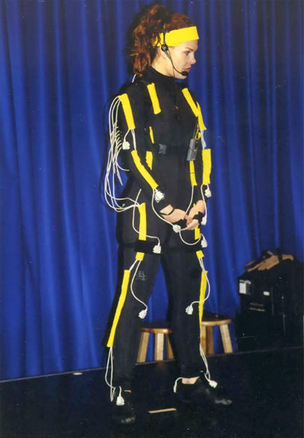
\includegraphics[width=0.22\textwidth]{figuras/monitorizacion/moni14}
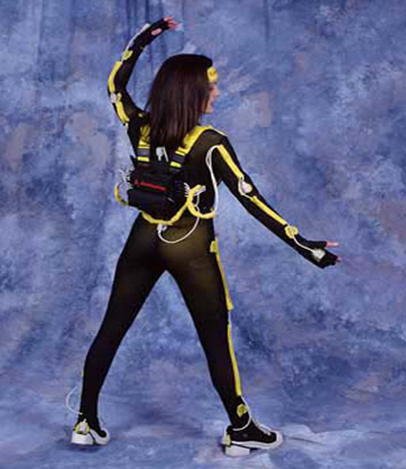
\includegraphics[width=0.274\textwidth]{figuras/monitorizacion/moni15}
\caption{Sistema magn�tico \cite{moni5}.}
\label{fig:moni15}
\end{figure}

\textbf{Sistemas ac�sticos}:

Este sistema consiste en un emisor de ondas sonoras de alta frecuencia y su sistema receptor correspondiente. El sistema receptor est� formado por tres micr�fonos en posici�n fija, y, a su vez, el sistema transmisor est� formado por tres transmisores tambi�n en posici�n fija. Las medidas pueden efectuarse atendiendo a la coherencia de fase o a medidas de tiempos. En el primer caso, las medidas de posici�n y orientaci�n se obtienen calculando el desfase entre la se�al transmitida y la recibida; por tanto, siempre que el objeto al que se le hace el seguimiento no se desplace una distancia superior a la longitud de onda de la se�al utilizada en el intervalo de tiempo entre una medici�n y otra, el resultado obtenido ser� correcto. En el segundo caso, se mide el tiempo que tarda el sonido emitido por el transmisor en un instante predeterminado en llegar al receptor; las medidas de posici�n s�lo requieren un transmisor, pero para medir orientaciones s� es necesario el uso del sistema emisor formado por tres transmisores de alta frecuencia. Un ejemplo de este tipo de sistemas se muestra en la figura \ref{fig:moni27}.


\begin{figure}[H]
\centering
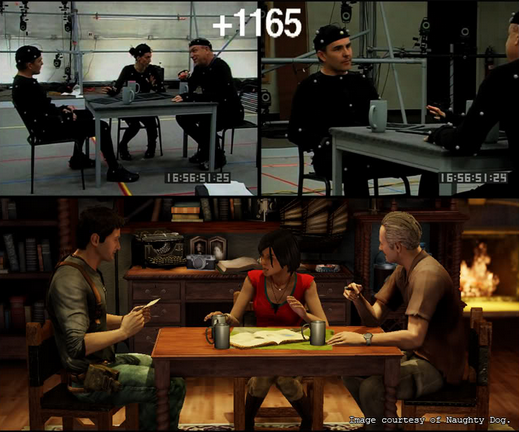
\includegraphics[width=0.42\textwidth]{figuras/monitorizacion/moni27}

\caption{Sistema ac�stico. Tecnolog�a usada por rockstar.}
\label{fig:moni27}
\end{figure}

\begin{itemize}
	\item Ventajas
	\begin{itemize}
	\item Muy preciso.
	
	\end{itemize}
	\item Incovenientes
	\begin{itemize}
		\item El cableado de los sensores hace a estos sistemas aparatosos y molestos a la hora de realizar movimientos amplios y/o r�pidos.
		\item Tienen un alcance limitado.
		\item El n�mero de sensores de este tipo que se pueden usar simult�neamente es limitado.
		\item Muy sensible a las condiciones ambientales de presi�n, humedad y temperatura.
		\item Muy sensible a las interferencias ac�sticas provocadas por los objetos del entorno, lo que implica en la pr�ctica que s�lo pueden ser usados en entornos muy controlados.
		
	\end{itemize}
\end{itemize}



\subsubsection{Sistemas de captura del movimiento �pticos}

\textbf{Sistemas �pticos basados en marcadores activos}

En estos sistemas, los marcadores son diodos LED (usualmente infrarrojos). Las c�maras no captan el reflejo de luz en los marcadores, sino que captan, directamente, la luz emitida por los marcadores.



Como quiera que estos marcadores han de emitir luz, necesitan disponer de una fuente de energ�a, a la que se conectan a trav�s de cables. Por ello, los sistemas HMC basados en marcadores activos son m�s aparatosos que los basados en marcadores pasivos, ya que la persona debe llevar puestos no s�lo los marcadores, sino tambi�n los codificadores, las bater�as y los cables que lo conectan todo. En la figura \ref{fig:moni25} se muestra un sistema de estas caracter�sticas.



\begin{figure}[H]
\centering
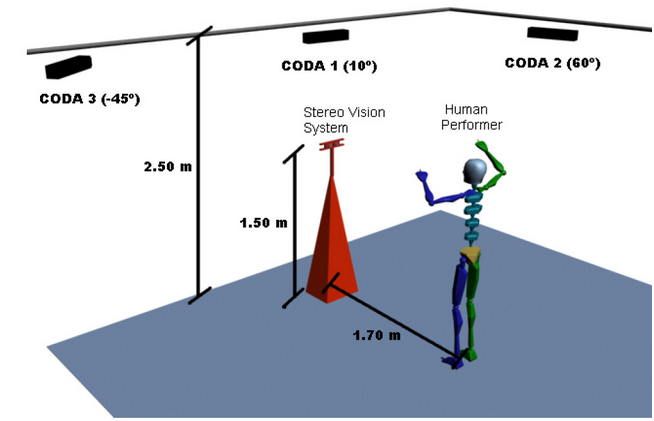
\includegraphics[width=0.52\textwidth]{figuras/monitorizacion/moni25}
\caption{Sistema CODAMotion \cite{moni5}.}
\label{fig:moni25}
\end{figure}


\begin{itemize}
	\item Ventajas
	\begin{itemize}
	\item Son muy precisos.
	\item Pueden capturar movimientos muy r�pidos (igual que los basados en marcadores pasivos).
	\item Son menos sensibles a interferencias producidas por fuentes de luz externas. Recientemente, por ejemplo, se ha empezado a comercializar un sistema de este tipo que funciona en exteriores.
	
	\end{itemize}
	\item Incovenientes
	\begin{itemize}
		\item Son caros.
		\item Requieren un entorno controlado amplio (volumen de captura).
		\item Los marcadores han de colocarse cuidadosamente sobre el usuario para evitar derivas entre pruebas.
		\item Hay que recalibrarlos frecuentemente.
		
		\item Son sensibles a oclusiones. De hecho, utilizar muchas c�maras es una forma, sobre todo, de intentar evitar las oclusiones de los marcadores.
		\item No hay forma de distinguir unos marcadores de otros. Es necesario un postprocesado, a veces tedioso, para inferir qu� marcador se corresponde con cada marca detectada.
		
	\end{itemize}
\end{itemize}


\textbf{Sistemas �pticos basados en marcadores pasivos}

En este caso, se emplean peque�os marcadores (usualmente esf�ricos) cubiertos de un material retrorreflector (un material que devuelve la luz que incide sobre �l hacia la fuente de luz, pr�cticamente sin dispersi�n espacial).



En estos sistemas, se colocan una serie de c�maras alrededor de los marcadores que se quieren capturar. Cada c�mara est� a su vez emparejada con un dispositivo emisor de luz, usualmente infrarroja. De hecho, la configuraci�n t�pica para estas c�maras es rodearlas de un anillo de LEDs infrarrojos, como se muestra en la figura \ref{fig:moni23} (donde los LEDs se ven rojos porque la emisi�n es en una banda de frecuencias centrada en el infrarrojo, pero que se extiende un poco al espectro visible).



\begin{figure}[H]
\centering
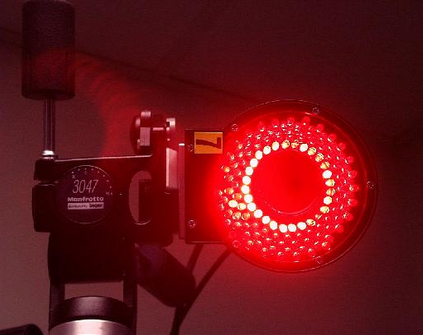
\includegraphics[width=0.32\textwidth]{figuras/monitorizacion/moni23}
\caption{C�mara rodeada de un anillo de LEDs infrarrojos \cite{moni5}.}
\label{fig:moni23}
\end{figure}

Cuando la luz emitida incide sobre el marcador retrorreflector, �sta se refleja directamente hacia la c�mara como en la figura \ref{fig:moni24}, con lo que el marcador aparece en la imagen como un punto brillante, que destaca respecto al resto. Utilizando un umbral de intensidad, es posible detectar en qu� p�xeles 2D de la imagen se han reflejado todos los marcadores presentes.




\begin{figure}[H]
\centering
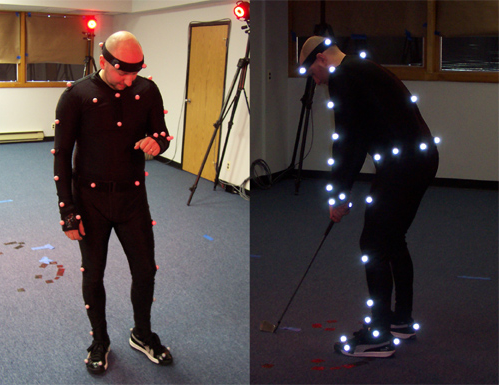
\includegraphics[width=0.32\textwidth]{figuras/monitorizacion/moni24}
\caption{Sistema de marcadores pasivos \cite{moni5}.}
\label{fig:moni24}
\end{figure}

\begin{itemize}
	\item Ventajas
	\begin{itemize}
	\item Son muy precisos.
	\item Pueden capturar movimientos muy r�pidos (la tasa de captura suele ser de 120 a 160 im�genes por segundo, aunque algunos sistemas pueden conseguir tasas de hasta 10000 im�genes por segundo en vol�menes reducidos).
	\item El usuario no tiene que portar cables, bater�as ni codificadores.
	
	\end{itemize}
	\item Incovenientes
	\begin{itemize}
	\item Son caros.
	\item Requieren un entorno controlado amplio (volumen de captura).
	\item Los marcadores han de colocarse cuidadosamente sobre el usuario para evitar derivas entre pruebas.
	\item Hay que recalibrarlos frecuentemente.
	\item Son sensibles a oclusiones. De hecho, utilizar muchas c�maras es una forma, sobre todo, de intentar evitar las oclusiones de los marcadores.
	\item No hay forma de distinguir unos marcadores de otros. Es necesario un postprocesado, a veces tedioso, para inferir qu� marcador se corresponde con cada marca detectada.
		
	\end{itemize}
\end{itemize}


\textbf{Sistemas �pticos sin marcadores}


Los sistemas HMC anteriores son adecuados para grabar movimientos para una pel�cula o un videojuego, o para monitorizar la evoluci�n de un paciente en procesos de rehabilitaci�n. Sin embargo, si se quiere crear un interfaz para el ordenador basado en gestos, o controlar la televisi�n con movimientos de la mano, no se puede exigir al usuario que se coloque marcadores por el cuerpo, y que calibre un anillo de c�maras. Por otro lado, �qui�n demostrar�a nuevas tareas a un robot social, si para ello ha de acudir a una sala espec�fica, colocarse un traje de marcadores, calibrar c�maras y postprocesar los datos?

El problema de los sistemas HMC �pticos que no usan marcadores es, precisamente, que tienen que arregl�rselas para extraer la pose sin marcas. Para conseguirlo, han de ejecutar complejos algoritmos de filtrado, reconocimiento, clasificaci�n, aprendizaje o emparejamiento. Estos algoritmos consumen recursos, y tienden a requerir bastante tiempo para completarse. As�, uno de los mayores inconvenientes de los sistemas HMC �pticos sin marcadores es el de su limitada velocidad. El otro gran inconveniente de estos sistemas es su imprecisi�n: por mucho que se refinen los algoritmos de extracci�n de pose, sus resultados no mejorar�n la precisi�n que da un marcador �ptico.

\section{Estado del arte}

Tal y como adelantamos en el apartado anterior,  vamos a hacer un barrido de algunos de los dispositivos asociados a la monitorizaci�n del cuerpo humano presentes en la actualidad. Nos centraremos en dos tipos principalmente: los  de dispositivos   fundamentados en sensores inerciales (IMUs y MIMUs) y los dispositivos basados en c�maras.





\subsection{Sistemas basados en sensores inerciales}

Para situarnos mejor definiremos lo que es una IMU:
 
Una unidad de medici�n inercial o IMU (del ingl�s inertial measurement unit) \cite{moni6}, es un dispositivo electr�nico que mide e informa acerca de la velocidad, orientaci�n y fuerzas gravitacionales de un cuerpo que se mueve en el espacio, usando una combinaci�n de aceler�metros y gir�scopos. Adem�s existe la posibilidad de combinarlos con magnet�metros, en ese caso el dispositivo pasa a llamarse MIMU. Las unidades de medici�n inercial son normalmente usadas para maniobrar aviones, incluyendo veh�culos a�reos no tripulados, entre muchos otros usos, y adem�s naves espaciales, incluyendo transbordadores, sat�lites y aterrizadores. 

La IMU es el componente principal de los sistemas de navegaci�n inercial usados en aviones, naves espaciales, buques y misiles guiados entre otros. En este uso, los datos recolectados por los sensores de una IMU permiten a un computador seguir la posici�n del aparato, usando un m�todo conocido como navegaci�n por estima.

A continuaci�n se enumeran algunas de las MIMUs que pueden ser encontradas en el mercado:


\subsubsection{3DN-GX4-45   (\textit{Microstrain})}

El 3DM-GX4-45 \cite{moni7} es una miniatura de un tipo de Sistema de Navegaci�n Inercial(GPS/INS), que utiliza la tecnolog�a m�s avanzada de sensores MEMS. Combina un aceler�metro triaxial, un gir�scopo triaxial, un magnet�metro triaxial, sensores de temperatura, un alt�metro barom�trico, un procesador de doble n�cleo que ejecutan el \textit{Filtro de Kalman Extendido} (EKF) para proporcionar la posici�n, velocidad y la estimaci�n de la orientaci�n de forma precisa. Su factor de forma, rango de temperatura, supervivencia a choques, bias estable, rendimiento ante las vibraciones, bajo consumo y rendimiento se combinan para ser uno de los mejores GPS/INS en su clase. La figura \ref{fig:moni16} muestra el dispositivo.

\begin{figure}[H]
\centering
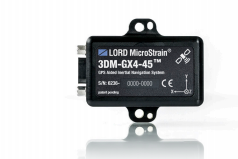
\includegraphics[width=0.32\textwidth]{figuras/monitorizacion/moni16}
\caption{3DN-GX4-45 \cite{moni7}.}
\label{fig:moni16}
\end{figure}

\subsubsection{Xsens MVN}

Xsens MVN \cite{moni8} es una soluci�n para todo el cuerpo, se basa en la captura del movimiento sin c�mara (MoCap). Consta de sensores inerciales adheridos al cuerpo por un traje de lycra (tambi�n disponible en tiras). Xsens MVN da libertad de movimiento porque no utiliza c�maras. Se trata de un sistema de captura port�til que se puede utilizar en interiores y al aire libre. Se caracteriza por su facilidad de uso y un tiempo de calibraci�n corto que permite configurar el sistema en menos de 15 minutos. En la figura \ref{fig:moni17} se puede ver Xsens MVN.


\begin{figure}[H]
\centering
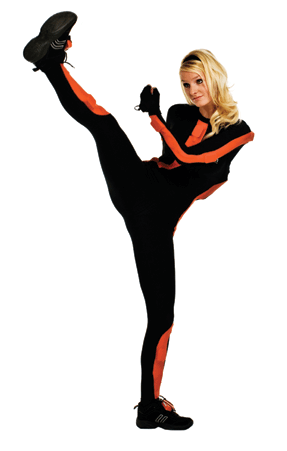
\includegraphics[width=0.20\textwidth]{figuras/monitorizacion/moni17}
\caption{Xsens MVN \cite{moni8}.}
\label{fig:moni17}
\end{figure}

Los datos resultantes de la captura del movimiento pueden ser utilizados para animar personajes digitales en pel�culas, juegos, cuentos animados, anuncios,etc. Tambi�n pueden ser utilizados en aplicaciones m�dicas y de entretenimiento para analizar el movimiento.


El traje MVN  de captura del movimiento que se muestra en la figura \ref{fig:moni18} presenta las siguientes caracter�sticas:

\begin{itemize}
	\item Seguimiento 6DOF (Degrees of Freedom) del cuerpo.
	\item 17  rastreadores inerciales MTx.
	\item Funcionamiento inal�mbrico de plena libertad de circulaci�n.
	\item Traje de lycra c�modo con cableado integrado.
	
\end{itemize}


\begin{figure}[H]
\centering
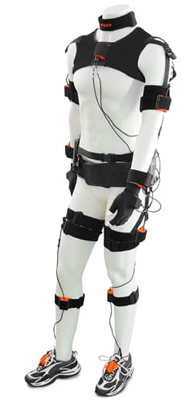
\includegraphics[width=0.20\textwidth]{figuras/monitorizacion/moni18}
\caption{Traje Xsens MVN \cite{moni8}.}
\label{fig:moni18}
\end{figure}


\subsubsection{9 DOF-Sensor Stick (\textit{SparkFun})}

Los giroscopos y los aceler�metros son bastante pr�cticos, pero por s� solos no dan la suficiente informaci�n para poder calcular c�modamente variables como la orientaci�n, la posici�n o la velocidad. Para medir esas y otras variables se suelen combinar los dos sensores, para crear una unidad de medici�n inercial (IMU) que proporciona seis grados de libertad (DOF). Tambi�n cabe la posibilidad de a�adir un magnet�metro pasando a tener nueve grados de libertad obteniendo una informaci�n m�s completa. Las IMUs son ampliamente utilizados en dispositivos que requieren el conocimiento de su posici�n exacta, por ejemplo, los brazos r�b�ticos, misiles guiados y para el estudio del movimiento del cuerpo humano. 


 9 DOF-Sensor Stick \cite{moni9} es una placa de sensores muy peque�a, con 9 grados de libertad.En la figura \ref{fig:moni19} se puede ver el dispositivo. Incluye aceler�metro ADXL345, el magnet�metro HMC5883L y el gir�scopo MEMS ITG-3200. El "Stick" tiene una interfaz I2C simple y un agujero de montaje para instalarla en tu proyecto. Adem�s, el tablero es un mero 0.036" de espesor, lo que le permite ser montado f�cilmente en casi cualquier aplicaci�n.


\begin{figure}[H]
\centering
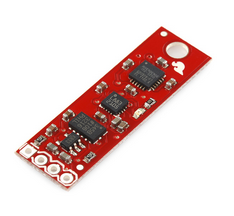
\includegraphics[width=0.20\textwidth]{figuras/monitorizacion/moni19}
\caption{T9 DOF-Sensor Stick \cite{moni9}.}
\label{fig:moni19}
\end{figure}








\subsection{Sistemas basados en c�maras}


Seg�n la clasificaci�n que establecimos en el apartado anterior, los sistemas basados en c�maras forman parte de los dispostivos �pticos de captura del movimiento humano. Vamos a describir a continuaci�n algunos de ellos:

\subsubsection {VICON 621}

Vicon 621 \cite{moni10} es un sistema �ptico de captura de tridimensional de movimiento que utiliza marcadores esf�ricos reflectantes y c�maras con antorchas de luz infrarroja  que recogen la reflexi�n infrarroja de los marcadores. Para el estudio cinem�tico es necesario colocar los marcadores sobre el sujeto, cuyo movimiento es captado por 6 c�maras, y analizado por triangulaci�n para obtener sus posiciones 3D reales fotograma a fotograma, generando as� un conjunto de datos de movimiento. El sistema es capaz de realizar simult�neamente el an�lisis electromiogr�fico de la actividad muscular. El sistema se muestra en la figura \ref{fig:moni20}.

\begin{figure}[H]
\centering
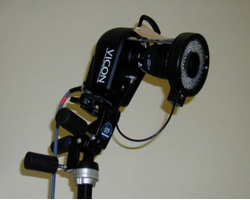
\includegraphics[width=0.3\textwidth]{figuras/monitorizacion/moni20}
\caption{VICON 621 \cite{moni10}.}
\label{fig:moni20}
\end{figure}



VICON 621 est� compuesto por:
 
 
\begin{itemize}
\item 6  c�maras de captura de la imagen de 50 Hz.
\item 6  canales activos de v�deo.
\item Electromi�grafo de 12 canales con conexi�n mediante fibra �ptica.
\item Software BODYBUILDER, para creaci�n, visualizaci�n y an�lisis de modelos cinem�ticos y cin�ticos. 
\item Software POLYGON para generaci�n de informes.
\item Estaci�n de trabajo basada en PC de �ltima generaci�n e impresora.
\item Sistema de captura de v�deo sincronizado. 
\end{itemize}
 
 
A contiuaci�n se puede ver la figura  \ref{fig:moni21} que muestra los marcadores del sistema VICON 621 colocados sobre una persona.
\begin{figure}[H]
\centering
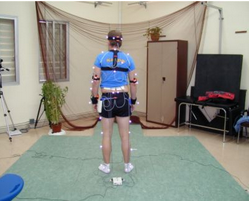
\includegraphics[width=0.3\textwidth]{figuras/monitorizacion/moni21}
\caption{VICON 621: Marcadores \cite{moni10}.}
\label{fig:moni21}
\end{figure}


\subsubsection{Oqus Camera series (Qualisys)}

La plataforma Oqus \cite{moni11} ofrece c�maras de captura de movimiento adecuadas para todas las aplicaciones posibles, tanto en interiores como al aire libre, como la que se puede ver en la figura \ref{fig:moni22}. Las c�maras Oqus est�n dise�adas para capturar datos \textit{mocap} precisos con una latencia muy baja y trabaja con marcadores pasivos y activos.

La caracter�stica principal de las c�maras Oqus es la capacidad de calcular posiciones de marcador con impresionante precisi�n y velocidad. Cientos de marcadores se pueden medir en miles de im�genes por segundo con diez, cincuenta o incluso m�s c�maras - descargadas en un port�til com�n. No es necesario el uso de estaciones de trabajo. No se necesita ning�n centro externo. El sistema aporta movilidad y es muy f�cil de configurar.


\begin{figure}[H]
\centering
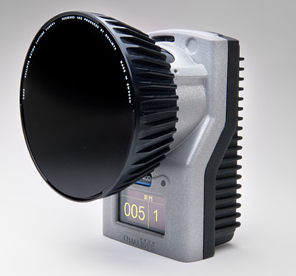
\includegraphics[width=0.3\textwidth]{figuras/monitorizacion/moni22}
\caption{Oqus Camera series \cite{moni11}.}
\label{fig:moni22}
\end{figure}



Caracter�sticas principales:

\begin{itemize}
\item Captura de movimiento de alta velocidad.
\item V�deo de alta velocidad.
\item Resoluciones del sensor: 0.3, 1.3, 4 y 12 megap�xeles.
\item Filtro activo para mediciones en exteriores.
\item Lentes motorizadas.
\item Soporte para marcadores activos.
\item Arquitectura de tiempo real para una baja lantencia.
\item Comunicaci�n inal�mbrica.
\item N�mero de c�maras/marcadores ilimitado.
\item Silencioso, sin ventilador.


\end{itemize}




\subsubsection {Kinect}


El Kinect \cite{moni12} es un dispositivo de la consola de juegos Xbox de Microsoft que permite interactuar con la consola sin necesidad de tener un contacto f�sico con un controlador de video-juegos tradicional. Este dispositivo permite interactuar con el videojuego mediante la captura del moviento del cuerpo, fue desarrollado por microsoft y sus librerias son de f�cil acceso para implentar este dispositivo en otras aplicaciones. La figura \ref{fig:moni28} muestra la imagen del dispositivo Kinect.

\vspace{25 mm}

\begin{figure}[H]
\centering
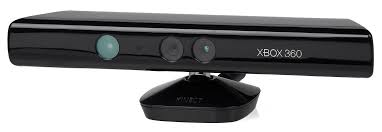
\includegraphics[width=0.4\textwidth]{figuras/monitorizacion/moni28}
\caption{Kinect Xbox 360 \cite{moni14}.}
\label{fig:moni28}
\end{figure}

\vspace{10mm}

A continuaci�n se enumeran las caracter�sticas principales del Kinect Xbox 360:

\vspace{10mm}

\textbf{Sensores}

\begin{itemize}
\item Lentes de color y sensaci�n de profundidad.
\item Micr�fono multi-arreglo.
\item Ajuste de sensor con su motor de inclinaci�n.
\item Totalmente compatible con las consolas existentes de Xbox 360.
\end{itemize}

\textbf{Campo de visi�n}

\begin{itemize}
\item Campo de visi�n horizontal: 57 grados.
\item Campo de visi�n vertical: 43 grados.
\item Rango de inclinaci�n f�sica: $\pm $ 27 grados.
\item Rango de profundidad  del sensor: 1,2 - 3,5 metros.
\end{itemize}

\textbf{Streams (Flujo de datos)}

\begin{itemize}
\item 320 $\times$ 240 a 16 bits de profundidad @ 30fps.
\item 640 $\times$ 480 32-bit de color @30fps.
\item Audio de 16-bit @ 16 kHz.

\end{itemize}

\textbf{Sistema de Seguimiento}

\begin{itemize}
\item Rastrea hasta 6 personas, incluyendo 2 jugadores activos.
 
\item Rastrea 20 articulaciones por jugador activo.

\item Capacidad para mapear jugadores activos en Live Avatars.

\end{itemize}

\textbf{Sistema de audio}

\begin{itemize}

\item Chat en vivo y voz dentro del juego (requiere Xbox Live Gold).
\item Sistema de cancelaci�n de eco que aumenta la entrada de voz.
\item Reconocimiento de voz m�ltiple.

\end{itemize}














\clearemptydoublepage
\chapter{Hardware Description}
\label{ch:Hardware}
Along this chapter we will introduce a general description of all devices used to data gathering for the development of this project.


It should be noted at this point that there are two clearly differentiated parts. In the first of them, we work with Force Plate and GaitWatch data, taking out their characteristic signals and synchronising them. In the second of them, we work jointly with Gait Watch and Qualisys System data for the purpose of comparing the accuracy in the calculated orientation angles.


\section{GaitWatch}

GaitWatch is an Inertial Measurement Unit (IMU) designed for gait monitoring of patients. It was developed by Prof. Dr. Med. Kai B¨otzel at the Department of Neurology of Ludwig-Maximilians University in Munich in conjunction with Dr. Alberto Olivares Vicente from the Department of Signal Theory, Telematics and Communications of the University of Granada. \cite{OlivaresBotzel2013}

The system is composed of the central processing unit and
a set of measuring units which are wired to it. The measuring units are 
placed in the patients’ thighs, shanks, arms and trunk.

The central processing unit has a microcontroller is in charge of gathering the data from the external measurement units and writing it to the memory card. So, this central unit is placed in the trunk inside a box and it contains an AL-XAVRB board with an AVRATxmega processor which contains the necessary embedded firmware to gather the data from all the measurement units and store it in a microSD card. Also, the trunk box contains some embedded magnetic and inertial sensors.

There are three different kinds of external units with the following components:
\begin{itemize}
	\item Type A (thighs and shanks): 
	\begin{itemize}
		\item IMU 5 from Sparkfun. IMU 5 contains an IDG500  biaxial gyroscope (from which only Y axis is actually used) with a measurement range of $\pm500deg/s$ and a $\pm3g$ triaxial accelerometer, ADXL335 .
	\end{itemize}
	\item Type B (arms):
	\begin{itemize}
		\item IDG500  biaxial $\pm500deg/s$ gyroscope.
	\end{itemize}
	\item Type C (trunk box):
	\begin{itemize}
		\item ADXL345  triaxial accelerometer with programmable range ($\pm16g/\pm8g/\pm4g/\pm2g$).
		\item IMU3000 triaxial gyroscope with programmable range ($\pm250/\pm500/\pm1000/\pm3000 (deg/s)$).
		\item Micromag3  triaxial magnetometer ($\pm11Gauss$).
	\end{itemize}
\end{itemize}


\section{Force Platform}

\section{Qualisys System}


\clearemptydoublepage
\chapter{Fundamentos}
\label{ch:fundamentos}

En el Cap�tulo que vamos a ver a continuaci�n, se realizar� un extenso an�lisis a nivel te�rico de los fundamentos de los sensores inerciales (aceler�metro, gir�scopo y  magnet�metro) utilizados en los sitemas GaitWatch  y ECnsole. La segunda parte del cap�tulo se centrar� primero en  explicar el proceso de calibraci�n, cuyo objetivo es transformar los datos originales en unidades con sentido f�sico. Despu�s se describir�n los algoritmos para el c�lculo de la orientaci�n. Primero el m�todo de \textit{Integraci�n de la Velocidad Angular} para el gir�scopo. Posteriormente, el m�todo de \textit{Descomposici�n de la Gravedad} donde el aceler�metro y el magnet�metro trabajan de manera conjunta. Despu�s, el  \textit{Filtro de Kalman} que  fusiona  los datos   del aceler�metro, gir�scopo y manet�metro obteniendo unos resultados m�s precisos. Y por �ltimo, el \textit{Filtro de Kalman Extendido} (una mejora del \textit{Filtro de Kalman} gracias al uso de un elemento nuevo, los cuaterniones, que minimizan el c�lculo computacional).

\section{Fundamentos de sensores}

A continuaci\'on vamos a realizar una descripci\'on de los fundamentos b\'asicos de los sensores que forman parte de los dispositivos cuyos datos son representados por la aplicaci�n desarrollada.

\subsection{Aceler\'ometros}

Los aceler\'ometros \cite{funda1} son los sensores utilizados para medir la aceleraci\'on tal y  como su propio nombre indica. Es un instrumento que va unido a un objeto que permite medir la aceleraci\'on del mismo. La medida de la acelerac�on se consigue midiendo respecto a su masa inercial interna.

Este dispositivo nos permite saber en cada momento el valor de la segunda derivada del espacio y mide la fuerza de inercia que incide sobre una masa cuando es afectada por un cambio de velocidad.

 
Existen distintos tipos de tecnolog\'ias para medir la aceleraci�n: piezo-el\'etricos, piezo-resistivo, galgas extensom\'etricas, l\'aser, t\'ermico,etc. Adem�s se presentan tambi\'en gran variedad de dise�os en funci\'on de la aplicaci\'on a la que van a ser destinados o  las condiciones de trabajo del aceler\'ometro. 
 
Los dos par\'ametros principales que determinan la elecci\'on del medidor adecuado son los rangos de funcionamiento de temperatura y frecuencia. Existen otros par\'ametros a tener en cuenta, como el tama�o, la resistencia a golpes, el precio, etc.



Los aceler\'ometros han pasado de estar dedicados a un uso industrial (medir 
vibraciones y oscilaciones) y de investigaci\'on, a estar presentes en muchos aparatos 
cotidianos (Videoconsolas, smartphones, GPS, autom�viles, relojes).




Ahora vamos a describir algunos de los tipos de aceler�metros existentes. Esta informaci�n se ha extraido de \cite{funda2}, donde se hace un estudio en mayor profundidad.


\subsubsection{Aceler\'ometro mec\'anico}


Este tipo de aceler\'ometro es el m\'as simple. Est\'a formado por unas masas unidas a un dinam\'ometro que se encuentra en la misma direcci\'on en la que queremos medir.


Haciendo uso de la segunda Ley de Newton, definida por la ecuaci�n \ref{newton}:

\begin{equation}
\label{newton}
		F = ma
\end{equation}


donde \textit{F} es la fuerza resultante que act\'ua sobre la masa, y \textit{a}  es la aceleraci\'on.

A trav\'es de la f\'ormula se puede deducir el valor de la aceleraci\'on ya que el dinam\'ometro mide el m\'odulo de la fuerza.


\begin{equation}
		a = \frac{F}{m}
\end{equation}

La figura \ref{fig:Fundamentos14} nos muestra una aceler�metro de tipo mec�nico.

\vspace{5mm}

\begin{figure}[H]
\centering
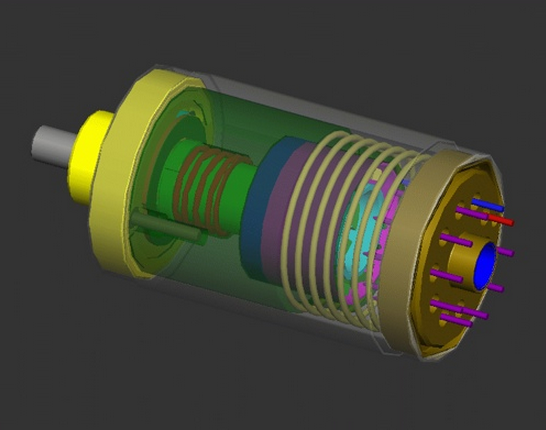
\includegraphics[width=0.25\textwidth]{figuras/Fundamentos/Fundamentos14}
\caption{Aceler�mentro mec�nico \cite{funda14}.}
\label{fig:Fundamentos14}
\end{figure}


\subsubsection{Aceler\'ometro piezoel\'ectrico}
 
 
 El aceler\'ometro piezoel\'etrico  est\'a basado en un ret\'iculo cristalino piezoel\'etrico y el cual se comprime produciendo una carga el\'ectrica proporcional a la fuerza aplicada.
 
 El material utilizado para los elementos piezoel\'etricos suele ser el circonato de plomo. La estructura del aceler\'ometro es una caja met\'alica y en el interior se encuentran los elementos  piezoel\'etricos. �stos est�n comprimidos por una masa sujeta a otro lado por un muelle. Al exponer el conjunto a una vibraci\'on, el disco piezoel\'ectrico se ve sometido a una fuerza variable que es proporcional a la aceleraci\'on de la masa. Gracias al efecto piezoel\'ectrico se genera una carga proporcional a la fuerza y por consiguiente a la aceleraci\'on. Haciendo uso de un volt\'imetro se puede medir el potencial.
 
Uno de los usos m\'as comunes es el mantenimiento predictivo, detectando defectos en m\'aquinas rotativas y alternativas.

La figura \ref{fig:Fundamentos16} muestra un aceler�metro de tipo piezoel�ctico.

\begin{figure}[H]
\centering
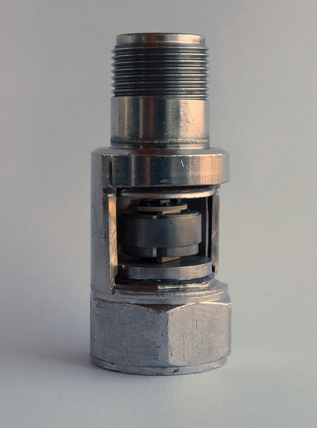
\includegraphics[width=0.2\textwidth]{figuras/Fundamentos/Fundamentos16}
\caption{Aceler�mentro piezoel�ctrico \cite{funda15}.}
\label{fig:Fundamentos16}
\end{figure}


\subsubsection{Otros tipos de aceler\'ometros}
 
 
\paragraph{Aceler\'ometro de efecto Hall.}

Est\'a fundamentado en la detecci\'on del campo magn\'etico a trav\'es de un sensor de efecto Hall. Para ello se utiliza una masa s\'ismica donde se coloca un im\'an y este tipo de sensor. En la figura \ref{fig:Fundamentos18}  se puede ver un aceler�metro de efecto Hall.

\begin{figure}[H]
\centering
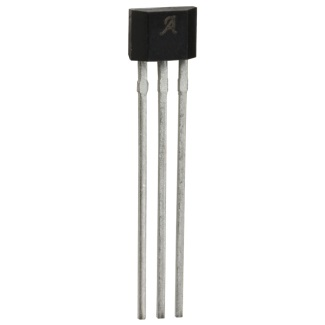
\includegraphics[width=0.2\textwidth]{figuras/Fundamentos/Fundamentos18}
\caption{Sensor de efecto Hall con salida lineal de proporci\'on \cite{funda16}.}
\label{fig:Fundamentos18}
\end{figure}

\paragraph{Aceler\'ometro de condensador.}

Mide el cambio de la capacidad de las placas de un circuito debido al movimiento de una masa s\'ismica interna que al desplazarse hace que cambie el valor de la corriente que pasa a trav\'es de las placas. La figura \ref{fig:Fundamentos17} representa un aceler�metro de este tipo.


\begin{figure}[H]
\centering
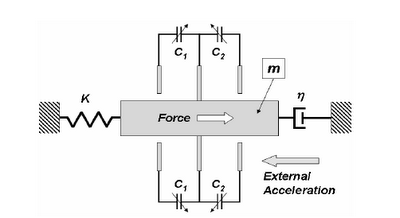
\includegraphics[width=0.5\textwidth]{figuras/Fundamentos/Fundamentos17}
\caption{Aceler�metro de condensador \cite{funda17}.}
\label{fig:Fundamentos17}
\end{figure}

\paragraph{Nuevas tecnolog\'ias.}

En la actualidad existen aceler\'ometros de 3 ejes.  Son construidos en un chip de silicio sobre el que se incluye la parte electr\'onica encargada del procesamiento de se�ales.

El fundamento f\'isico de estos sensores (tecnolog\'ia MEMS) est\'a basado en el traspaso t\'ermico por convecci\'on natural.

Las siglas MEMS \cite{funda6}, son en conjunto un acr�nimo para denotar a lo que actualmente se conoce como  Sistemas Micro Electro Mec�nicos, los cuales integran elementos mec�nicos, sensores, actuadores y dispositivos electr�nicos agrupados en su conjunto en un substrato u ''oblea'' com�n de silicio, mediante el uso de tecnolog�a aplicada en micro fabricaci�n.

Este tipo de aceler�metros son los utilizados en los sistemas GaitWatch y ECnsole.



\subsection{Gir\'oscopo}

 

El gir�scopo \cite{funda3} es una rueda giratoria cuyo eje puede cambiar de direcci�n. Como vemos en la figura \ref{fig:Fundamentos19}.

\begin{figure}[H]
\centering
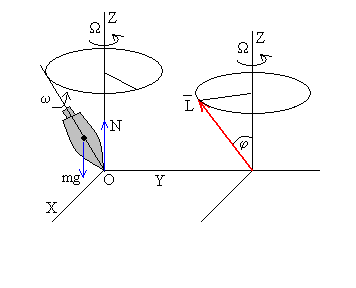
\includegraphics[width=0.5\textwidth]{figuras/Fundamentos/Fundamentos19}
\caption{Fundamentos del gir�scopo \cite{funda3}.}
\label{fig:Fundamentos19}
\end{figure}

En general, el vector momento angular \textbf{L} no tiene la direcci�n del eje de rotaci�n, es decir, el vector momento angular no coincide con su proyecci�n $ L_{z} $ a lo largo del eje de rotaci�n. Cuando coinciden se dice que el eje de rotaci�n es un eje principal de inercia.
Para estos ejes existe una relaci�n sencilla entre el momento angular \textbf{L} y la velocidad angular $ \boldsymbol{\omega} $, dos vectores que tienen la misma direcci�n, la del eje de rotaci�n
 
\begin{equation}
\mathbf{L}=I\boldsymbol{\omega}
\end{equation}

El t�rmino \textit{I} se denomina momento de inercia  y no es una cantidad caracter�stica como puede ser la masa o el volumen, sino que su valor depende de la posici�n del eje de rotaci�n. 





En ausencia de momento de fuerzas sobre el s�lido M, el cuerpo seguir� rotando con respecto a dicho eje con velocidad angular constante.

Si el momento aplicado sobre el s�lido en rotaci�n no es nulo, el momento angular experimenta un cambio en su direcci�n tal como se muestra en la figura.


\begin{equation}
		\mathbf{M}=\frac{\mathbf{dL}}{dt}
\end{equation}



Las fuerzas aplicadas sobre el s�lido en rotaci�n que se muestran en la figura \ref{fig:Fundamentos20} son:
\begin{itemize}
\item El peso \textit{mg} que act�a sobre el centro de masas, situado a una distancia \textit{b} del punto de apoyo O.
\item La reacci�n \textit{N} en el punto de apoyo O.
\end{itemize}



\begin{figure}[H]
\centering
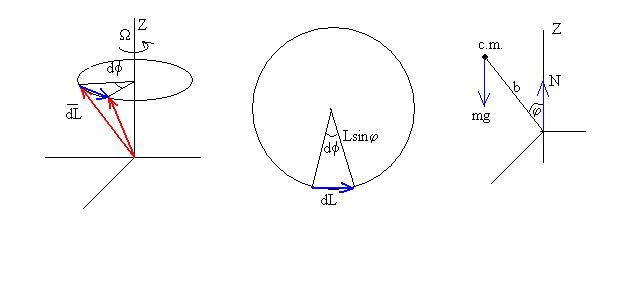
\includegraphics[width=0.7\textwidth]{figuras/Fundamentos/Fundamentos20}
\caption{Fuerzas aplicadas sobre el s�lido de rotaci�n \cite{funda3}.}
\label{fig:Fundamentos20}
\end{figure}


El momento \textbf{M} de las fuerzas respecto del punto fijo O viene dado por la ecuaci�n \ref{momento}:

\begin{equation}
\label{momento}
 \mathbf{M}= mgb\cdot sin\varphi
\end{equation}
 
El cambio de momento angular \textbf{dL} tiene la direcci�n del momento \textbf{M} de las fuerzas aplicadas respecto del punto de apoyo O, ya que el momento \textbf{M} es perpendicular al momento angular \textbf{L}, el cambio de momento angular \textbf{dL} es tambi�n perpendicular a \textbf{L}, y el momento angular \textbf{L} cambia de direcci�n pero no de m�dulo.


El extremo del vector momento angular \textbf{L} describe una circunferencia de radio $Lsin\varphi$, y en un intervalo de tiempo dt se desplaza un �ngulo $d\theta$;. El cambio de momento angular es $dL=L\sin\varphi\cdot d\theta$, de modo que,

		\begin{equation}
		Iw\cdot\sin\varphi\frac{d\phi}{dt} = mgb\sin\varphi
		\end{equation}
		
		
Se denomina velocidad angular de precesi�n $\Omega$ a		

		\begin{equation}	
		\Omega=\frac{d\phi}{dt}=\frac{mgb}{Iw}
	    \end{equation}


Cuando el punto de apoyo O coincide con el centro de masas b=0, el momento \textbf{M} de las fuerzas es cero y la velocidad angular de precesi�n $\Omega$ es nula. El eje del gir�scopo se mantiene fijo en el espacio.

Esta descripci�n es aproximada, siempre que la velocidad angular $\omega$, sea grande en comparaci�n con la velocidad angular de precesi�n $\Omega$.

Un an�lisis m�s detallado del problema indica que el s�lido tiene tres movimientos:


\begin{itemize}
\item  De rotaci�n alrededor de su eje principal de inercia con velocidad angular $\omega$.
\item De precesi�n alrededor del eje vertical Z, con velocidad angular $\Omega$.
\item De nutaci�n o de oscilaci�n del eje vertical entre dos c�rculos.
\end{itemize}

No solamente el movimiento de rotaci�n contribuye al momento angular L, como hemos supuesto, sino tambi�n y en menor medida, los movimientos de precesi�n y de nutaci�n, esto es lo que hace dif�cil el an�lisis detallado de este sistema mec�nico.

Los fen�menos girosc�picos tienen muchas aplicaciones: la tendencia de un gir�scopo a mantener el eje de rotaci�n fijo en el espacio en ausencia de momento es utilizado en la estabilizaci�n de los barcos y en los pilotos autom�ticos de los aviones. En la figura \ref{fig:Fundamentos15} mostr�mos la imagen de un gir�scopo.



\begin{figure}[H]
\centering
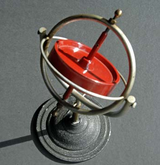
\includegraphics[width=0.3\textwidth]{figuras/Fundamentos/Fundamentos15}
\caption{Gir�scopo \cite{funda18}.}
\label{fig:Fundamentos15}
\end{figure}

Otro ejemplo interesante es la precesi�n de los equinoccios. El plano del ecuador hace un �ngulo de 23� 37' con el plano de la �rbita terrestre o ecl�ptica. La intersecci�n d elos dos planos es la l�nea de los equinoccios. La Tierra es un gir�scopo gigante cuyo eje de rotaci�n precesa alrededor del eje perpendicular al plano de la ecl�ptica con un periodo de 27725 a�os. La precesi�n de los equinoccios se debe al momento de las fuerzas ejercido por el Sol y la Luna sobre la Tierra.

\subsubsection{Gir�scopos MEMS}


Los gir�scopos MEMS \cite{funda7} (sistemas microelectromec�nicos) son los sensores utilizados por GaitWatch y ECnsole.  Este tipo de sensores sirve para medir la velocidad angular y se caracterizan por ser peque�os y de bajo coste. Las unidades de velocidad angular se miden en grados por segundo (� / s) o revoluciones por segundo (RPS). La velocidad angular es simplemente una medida de la velocidad de rotaci�n.


\begin{figure}[H]
\centering
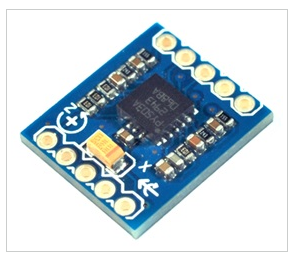
\includegraphics[width=0.3\textwidth]{figuras/Fundamentos/Fundamentos24}
\caption{Gir�scopo MEMS \cite{funda7}.}
\label{fig:Fundamentos24}
\end{figure}


\textbf{�C�mo funciona el gir�scopo MEMS para detectar la velocidad angular?}

\vspace{10mm}

\begin{figure}[H]
\centering
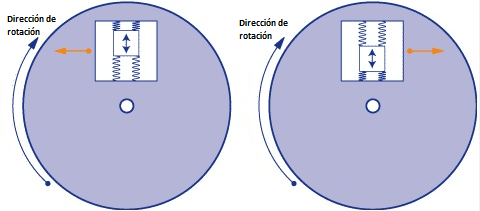
\includegraphics[width=0.6\textwidth]{figuras/Fundamentos/Fundamentos25}
\caption{Funcionamiento interno de un sensor girosc�pico MEMS \cite{funda7}.}
\label{fig:Fundamentos25}
\end{figure}

El sensor MEMS dentro de un giroscopio es muy peque�o (entre 1 a 100 micr�metros , el tama�o de un cabello humano). Cuando se hace girar el giroscopio, una peque�a masa de resonancia se desplaza con los cambios de velocidad angular. Este movimiento se convierte en se�ales el�ctricas de muy bajas corrientes que se pueden amplificar para ser le�das por un microcontrolador.

\subsection{Magnet�metro}	


Un magnet�metro \cite{funda4} es un sofisticado sensor que proporciona a los observadores cient�ficos una comprensi�n m�s clara de c�mo funciona el magnetismo.

La Tierra genera un campo magn�tico que crea disturbios magn�ticos medibles en la atm�sfera. Un magnet�metro es un instrumento cient�fico que mide este fen�meno en t�rminos de densidad de flujo magn�tico. La unidad cient�fica para la lectura de la densidad del flujo magn�tico es el Tesla, el Gauss o As/m2. Las sustancias y materiales que perturban este flujo se denominan magn�ticos. Cuando hay materiales magn�ticos presentes, un magnet�metro detecta la cantidad de distorsi�n que estos materiales causan en el campo de la Tierra. Un magnet�metro no s�lo nos dice c�mo afectan el flujo magn�tico ciertos materiales magn�ticos en particular, sino que tambi�n puede medir la fuerza de los campos magn�ticos. Esta informaci�n puede utilizarse para discernir la direcci�n, la rotaci�n y el �ngulo de los campos magn�ticos, as� como la ubicaci�n de objetos espec�ficos dentro de ellos.





\subsubsection{Magnet�metro de precesi�n de protones}

Un magnet�metro barato y port�til es el magnet�metro de precesi�n de protones. Este instrumento se utiliza principalmente en muestras cercanas a la superficie en estudios de ingenier�a y medioambientales. El magnet�metro de precesi�n de protones requiere el uso de un l�quido rico en �tomos de hidr�geno para producir la se�al de la precesi�n. Para ello, el queroseno es una de las mejores opciones. Las corrientes directas y los campos magn�ticos polarizan los �tomos, y el instrumento lee su frecuencia de precesi�n. Existen limitaciones para este tipo de magnet�metro, como su bajo nivel de sensibilidad y su alto consumo de potencia. Sin embargo, es ideal para la exploraci�n y el mapeo de tuber�as subterr�neas. La figura \ref{fig:Fundamentos21} muestra un magnet�metro de precesi�n de protones.

\begin{figure}[H]
\centering
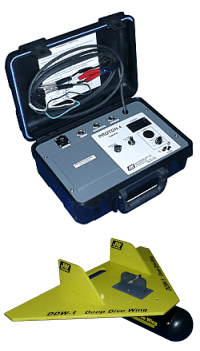
\includegraphics[width=0.15\textwidth]{figuras/Fundamentos/Fundamentos21}
\caption{Magnet�metro de precesi�n de protones \cite{funda19}.}
\label{fig:Fundamentos21}
\end{figure}


\subsubsection{Magnet�metro cu�ntico}

Magnet�metros cu�nticos son ampliamente utilizados en estudios ambientales, exploraci�n geof�sica, detecci�n de armas y otras aplicaciones cient�ficas. Estos instrumentos miden la magnitud espec�fica de los campos magn�ticos. Las part�culas subat�micas son polarizadas por los magnet�metros cu�nticos, lo que hace que se procesen alrededor de los campos magn�ticos de la Tierra. Esta polarizaci�n produce un patr�n reconocible que puede ser cuantificado y medido como un momento magn�tico. Estos momentos magn�ticos, referenciados con el campo magn�tico de la Tierra proporcionan informaci�n sobre la densidad del flujo magn�tico. La figura \ref{fig:Fundamentos22} muestra un magnet�metro cu�ntico.


\begin{figure}[H]
\centering
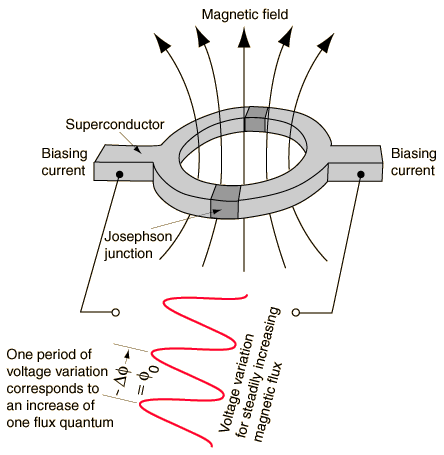
\includegraphics[width=0.3\textwidth]{figuras/Fundamentos/Fundamentos22}
\caption{Magnet�metro cu�ntico \cite{funda20}.}
\label{fig:Fundamentos22}
\end{figure}

\subsubsection{Magnet�metros vectoriales}

Adem�s de tener una magnitud, el flujo magn�tico tambi�n tiene una direcci�n o vector. Los magnet�metros vectoriales miden las propiedades del campo magn�tico que viajan en una determinada direcci�n. Estos instrumentos ofrecen una lectura m�s precisa de la densidad del flujo magn�tico al eliminar la sensibilidad cruzada y funcionar con un nivel de ruido muy bajo. Los magnet�metros vectoriales se han utilizado en naves espaciales desde 1988. Mediante los magnet�metros vectoriales, los sat�lites pueden incluso medir los campos magn�ticos de otros planetas y lunas.



Los magnet�metros pueden ser instrumentos �tiles en muchas aplicaciones profesionales. Al ser ligeros y port�tiles, los magnet�metros se transportan f�cilmente a casi cualquier sitio. En arqueolog�a, se pueden utilizar magnet�metros para localizar tumbas enterradas que contengan artefactos met�licos. En aplicaciones militares, los magnet�metros se utilizan para localizar los tanques, minas y los dep�sitos de combustible. La industria minera y otros numerosos campos cient�ficos tambi�n miden anomal�as magn�ticas con magnet�metros. La figura \ref{fig:Fundamentos23} muestra un magnet�metro vectorial.


\begin{figure}[H]
\centering
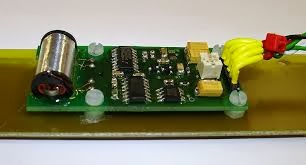
\includegraphics[width=0.5\textwidth]{figuras/Fundamentos/Fundamentos23}
\caption{Magnet�metro vectorial \cite{funda21}.}
\label{fig:Fundamentos23}
\end{figure}
 

\subsubsection{Magnet�metros MEMS}

Los magnet�metros MEMS son los utilizados en los dispositivos ECnsole y GaitWatch, por esta raz�n, se analizar� su funcionamiento (en la mayor�a de estos sensores predomina el uso de la fuerza de Lorentz) posteriormente. La figura \ref{fig:Fundamentos26} muestra un ejemplo de magnet�metro MEMS. 


\begin{figure}[H]
\centering
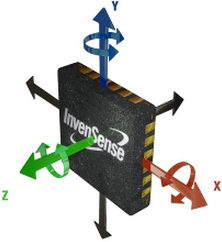
\includegraphics[width=0.35\textwidth]{figuras/Fundamentos/Fundamentos26}
\caption{Magnet�metro MEMS \cite{funda8}.}
\label{fig:Fundamentos26}
\end{figure}


\textbf{�C�mo funcionan los sensores MEMS basados en la fuerza de Lorentz?}

 Este tipo de sensores magn�ticos \cite{funda9} se basan en el movimiento mec�nico de la estructura MEMS,  es provocado por la fuerza de Lorentz que act�a sobre un conductor portador de la corriente situado en el interior del campo magn�tico. El movimiento mec�nico de la microestructura se detecta electr�nicamente o de forma �ptica.  Los m�todos de transducci�n piezorresistivo y electroest�tico se pueden utilizar en la detecci�n electr�nica; y  por otro lado, la medici�n del desplazamiento con fuente l�ser o fuente LED  se pueden utilizar para la detecci�n �ptica. Cabe resaltar que la estructura mec�nica es inducida a alcanzar su frecuencia de resonancia a menudo con el fin de obtener la se�al de salida m�xima.
 
 
\section{Fundamentos de la monitorizaci�n}

Una vez presentados los fundamentos de los sensores que contienen GaitWatch y ECnsole, vamos a proceder a explicar el procedimiento de calibraci�n de los datos medidos por los mismos.

\subsection{Calibraci�n}

El objetivo principal del proceso de calibraci�n consiste en transformar los datos en bruto en unidades con sentido f�sico.


En este apartado vamos a ver como se realiza el proceso de calibraci�n de los sensores que forman parte de dispositivo GaitWatch. No es necesario especificar el modo de calibraci�n para el sistema ECnsole ya que los sensores que componen el dispositivo reunen caracter�sticas similares y el procedimiento de calibraci�n es el mismo. Sin embargo difieren en el n�mero de sensores, como se puede ver en la tabla \ref{tab:sensores}:



\begin{table}[h]
	\caption{Lista de sensores que componen los sistemas GaitWatch y ECnsole}	
	\centering
		\begin{tabular}{|c|c|c|}\hline
		\label{tab:sensores}
		& \textbf{GaitWatch}				& \textbf{ECnsole} 	 	\\ \hline
		\textbf{Aceler�metro triaxial} & S�			& S�  		\\ \hline
		\textbf{Aceler�metro uniaxial}	& S�			& No  		\\ \hline
		\textbf{Gir�scopo triaxial} & S�			& S� 				\\ \hline
		\textbf{Gir�scopo uniaxial} & S�			& No 				\\ \hline
		\textbf{Magnet�metro triaxial}	& S�		& S�  				\\ \hline
		\end{tabular}
		
		
\end{table}


Las pautas para llevar a cabo el proceso de calibraci�n vienen recogidas en \cite{funda5} donde se realiza una descripci�n m�s exhaustiva del procedimiento.


\subsubsection{Calibraci�n del aceler�metro}

La calibraci�n de los aceler�metros est� dividida en dos partes de acuerdo con el n�mero  de ejes del aceler�metro. En el caso  del aceler�metro triaxial (incluido en el m�dulo de GaitWatch que se coloca en el tronco del paciente y en las plantillas para el sistema ECnsole) utilizaremos el algoritmo de ajuste elipsoidal de Camps et al. \cite{funda10} los cuales  presentaron un m�todo te�rico y experimental para calcular ganancias, bias y factores de no ortogonalidad de los aceler�metros y los magnet�metros. Las maniobras de calibraci�n  implican una serie de rotaciones arbitrarias de la MIMU, por lo que el conjunto de maniobras para recopilar los datos es muy simple.

\begin{itemize}
	\item \textbf{Modelado del sensor}: El modelo de salida del sensor viene dado por:
	
	\begin{equation}
	\begin{bmatrix}
	v_{x}(t) \\
	v_{y}(t) \\
	v_{z}(t)	
	\end{bmatrix}
	=
	\begin{bmatrix}
	s_{x} & 0 & 0 \\
	0 & s_{y} & 0 \\
	0 & 0 & s_{z} 
	\end{bmatrix}
	\begin{bmatrix}
	m_{x}(t)\\
	m_{y}(t)\\
	m_{z}(t)
	\end{bmatrix}
	+
	\begin{bmatrix}
	b_{x}\\
	b_{y}\\
	b_{z}
	\end{bmatrix}
	+
	\begin{bmatrix}
	\epsilon_{x}\\
	\epsilon_{y}\\
	\epsilon_{z}
	\end{bmatrix}
	\end{equation}


donde \textbf{b}=$(b_{x},\,b_{y},\,b_{z})^{T}$ representa el desplazamiento, $ s_{x} $,$ s_{y} $,$ s_{z} $ son las ganancias de los sensores, $ m_{x}(t) $, $ m_{y}(t) $, $ m_{z}(t) $ son los componentes de los actuales campos magn�ticos y gravitatorios y $ \epsilon_{x} $, $ \epsilon_{y} $,$ \epsilon_{z} $ son los componentes  del ruido para cada eje.

Si tomamos en consideraci�n los efectos de la no ortogonalidad, entonces la salida del sensor viene dada por:

\begin{equation}
\begin{bmatrix}
v_{x}(t) \\
v_{y}(t) \\
v_{z}(t) \\
\end{bmatrix}
=
\begin{bmatrix}
s_{xx} & s_{xy} & s_{xz} \\
s_{xy} & s_{yy} & s_{yz} \\
s_{xz} & s_{yz} & s_{zz}
\end{bmatrix}
\end{equation}

donde $ s_{ij} $ para $ i\neq j $ representa los errores de ortogonalidad entre los ejes \textit{i} y \textit{j} del sensor. 


\item \textbf{Procedimiento de calibraci�n}: Usando el hecho de que la norma del vector de entrada $ \textbf{m}= [m_{x}(t) m_{y}(t) m_{z}(t)]^{T}$ es constante, la siguiente relaci�n es derivada:

\begin{equation}
\|\textbf{m}\|^{2}=m_{x}(t)^{2}+m_{y}(t)^{2}+m_{z}^{2}
\end{equation}

\begin{equation}
\label{eq:11}
\|\mathbf{h}\|^{2}=(\frac{v_{x}(t)-b_{x}}{s_{x}})^{2}+(\frac{v_{y}(t)-b_{y}}{s_{y}})^{2}+(\frac{v_{z}(t)-b_{z}}{s_{z}})^{2}
\end{equation}

donde \textbf{m}=$(m_{x}(t),\,m_{y}(t),\,m_{z}(t))^{T}$ es el vector de campo gravitatorio $ m_{x}(t) $, $ m_{y}(t) $, $ m_{z}(t) $ son los componentes de los actuales campos gravitatorios, \textbf{h}=$(h_{x}(t),\,h_{y}(t),\,h_{z}(t))^{T}$ es el vector del campo gravitatorio sin tener en cuenta los componentes del ruido para cada eje, $ v_{x}(t) $,$ v_{y}(t) $,$ v_{z}(t) $ son las componentes de la salida del sensor, \textbf{b}=$(b_{x},\,b_{y},\,b_{z})^{T}$ representa el desplazamiento, y  $ s_{x} $,$ s_{y} $,$ s_{z} $ son las ganancias de los sensores.

\vspace{1cm}

La ecuaci�n \ref{eq:11} es la ecuaci�n param�trica de una elipsoide con centro en \textbf{b} y semi-ejes $ s_{x} $,$ s_{y} $ y $ s_{z} $. Usando el sistema de ecuaciones formado por varias medidas de tiempo t, estimamos los par�metros a trav�s de la minimizaci�n no lineal cuadr�tica del error de la funci�n

\begin{equation}
e_{p}(t)=\|\mathbf{m}\|^{2}-(\mathbf{v}(t)- \mathbf{b})^{T}(S^{-1})^{2}(\mathbf{v}(t)-\mathbf{b})
\end{equation}


donde


\begin{equation}
S^{-1}=
\begin{bmatrix}
1/s_{xx} & 1/s_{xy} & 1/s_{xz} \\
1/s_{xy} & 1/s_{yy} & 1/s_{yz} \\
1/s_{xz} & 1/s_{yz} & 1/s_{zz} \\
\end{bmatrix}
\end{equation}


El coste de la funci�n $ e_{p} $(t) es cuadr�tico, y es minimizado iterativamente por el algoritmo de Levenberg-Marquardt \cite{funda11,funda12}.

\end{itemize}

En resumen, si el aceler�metro se sit�a en m�ltiples posiciones casi-est�ticas y aleatorias, los datos recogidos deben describir idealmente una esfera de radio igual a la magnitud del vector gravedad.

Por lo tanto, el primer paso de calibraci�n es recoger los datos de la aceleraci�n que ser�n usados para encontrar los par�metros de calibraci�n �ptimos. Como se dijo antes, necesitamos situar el m�dulo que contiene el aceler�metro en m�ltiples posiciones casi-est�ticas y aleatorias intentando cubrir todas las orientaciones. Ya que la transici�n de una posici�n casi-est�tica es la causa de que el aceler�metro mida aceleraciones lineales que interrumpen la aceleraci�n de la gravedad, no podemos tomar cada punto medido. Para evitar seleccionar valores de aceleraci�n lineal tenemos que aplicar un algoritmo que se capaz de detectar los instantes casi-est�ticos.
La figura \ref{fig:Fundamentos4} muestra la aceleraci�n triaxial medida en cada posici�n casi-est�tica, adem�s de la aceleraci�n lineal no deseada. Esta figuara tambi�n muestra la salida del algoritmo de detecci�n de los instantes casi-est�ticos.


\begin{figure}[H]
\centering
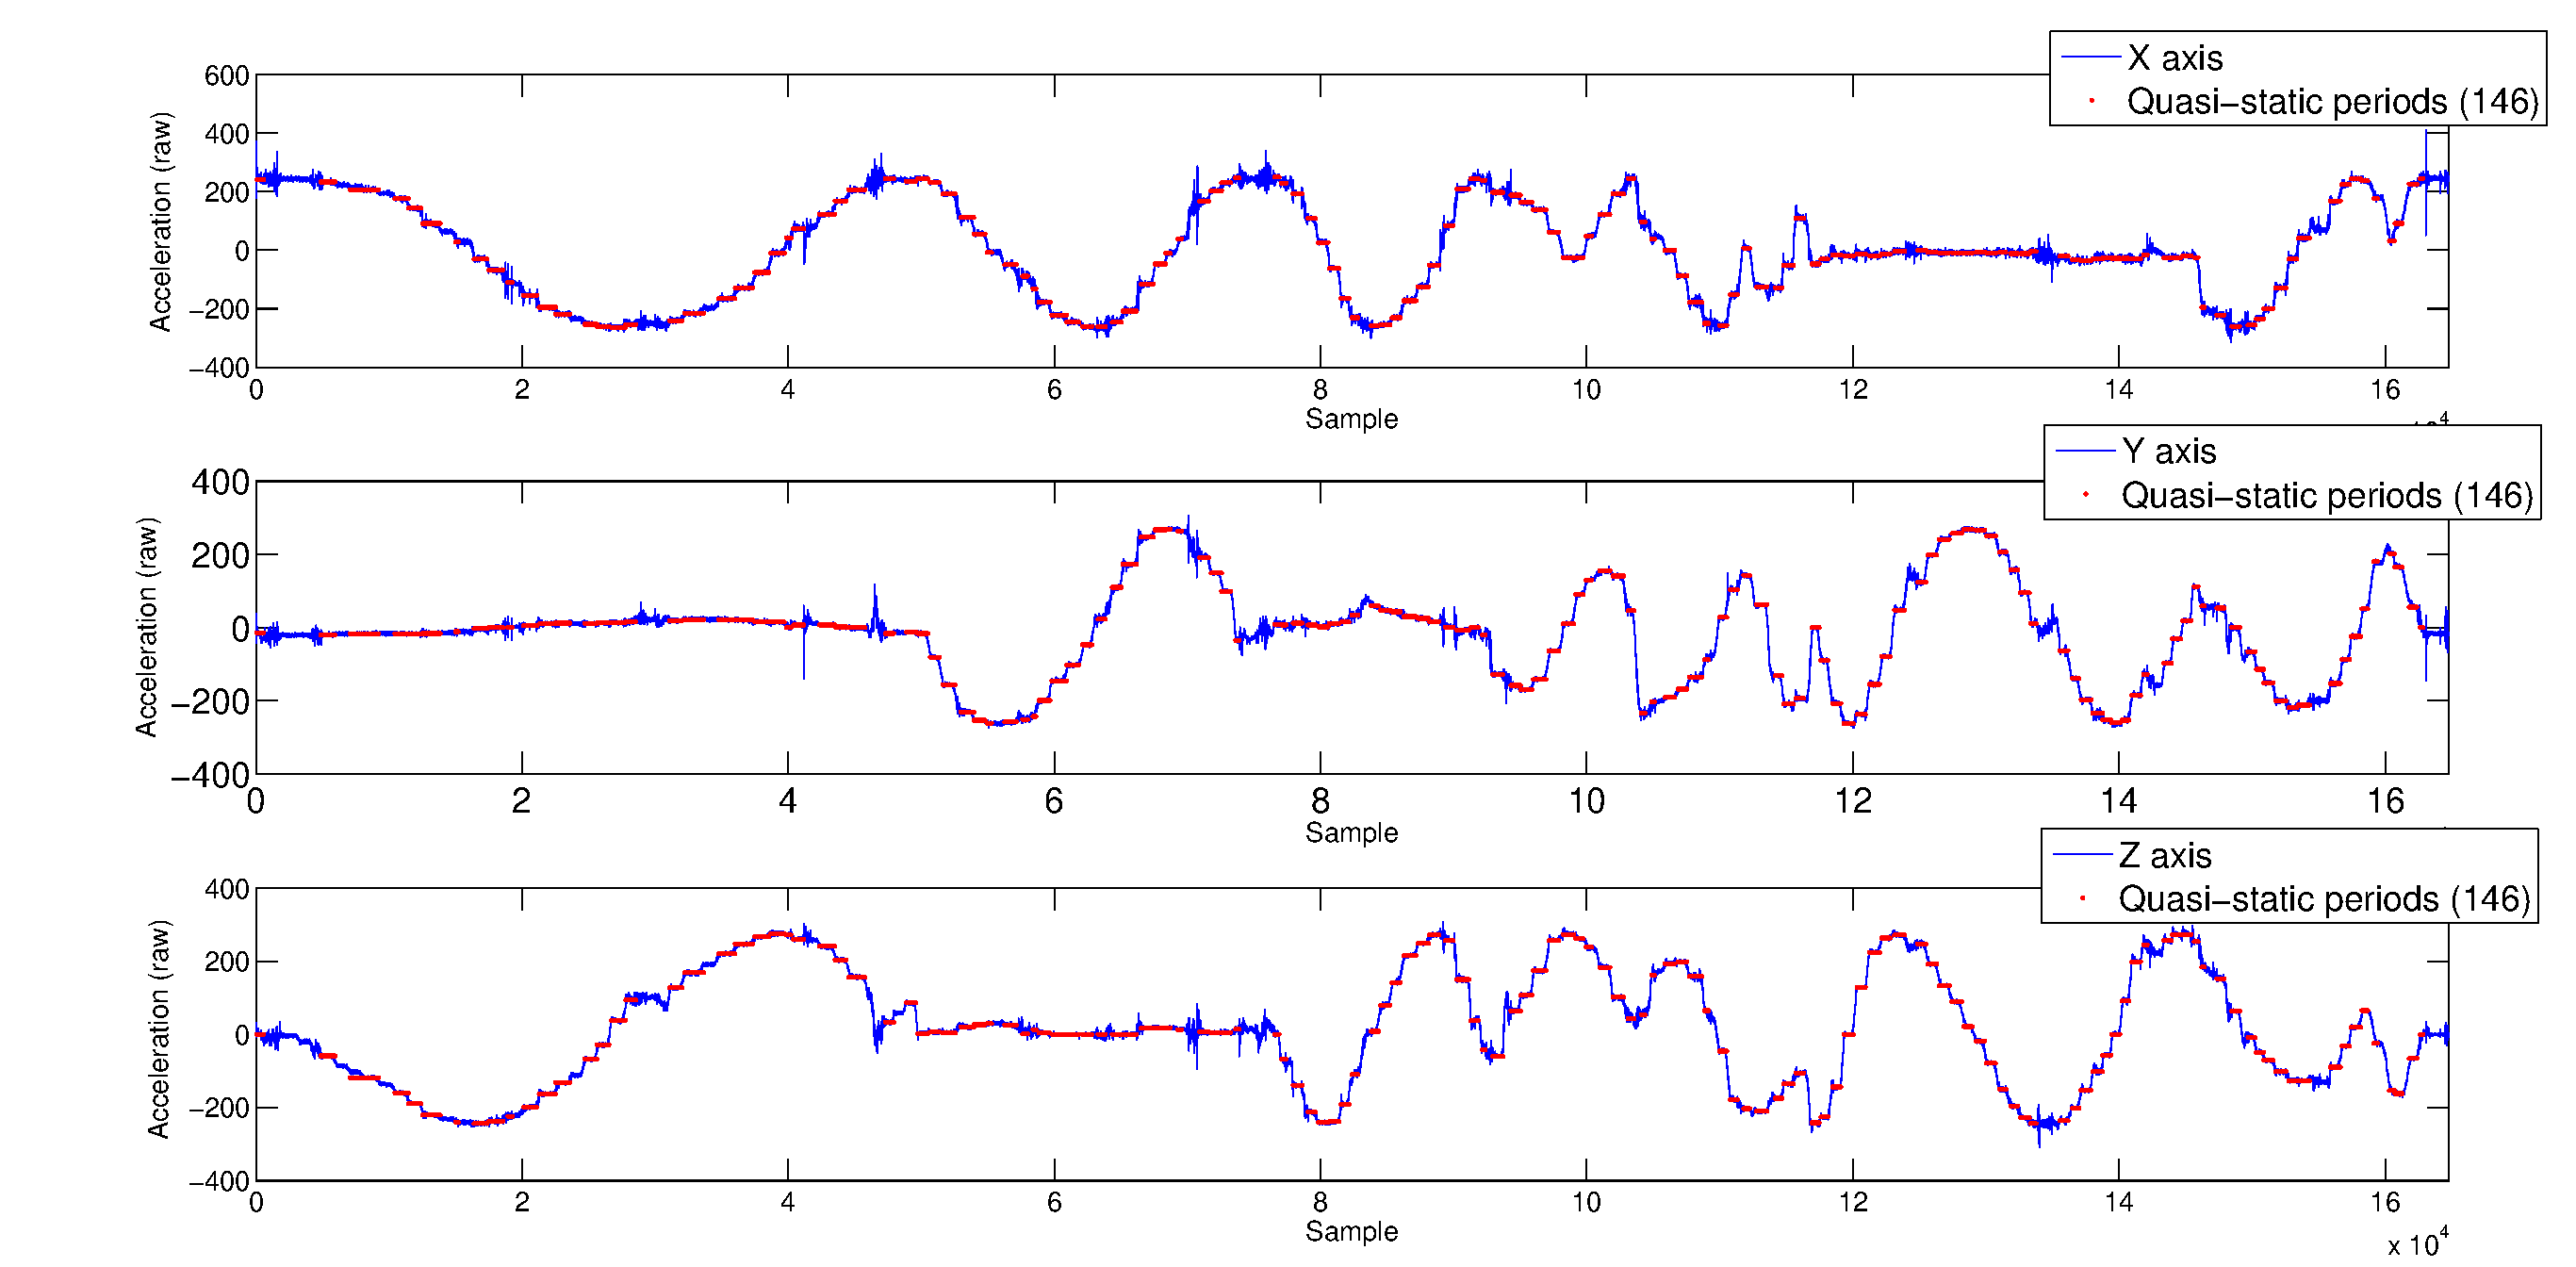
\includegraphics[width=0.9\textwidth]{figuras/Fundamentos/Fundamentos4EPS}
\caption{Aceleraci�n recogida en las posiciones casi-est�ticas y salida del algoritmo de detecci�n}
\label{fig:Fundamentos4}
\end{figure}

Si trazamos las aceleraciones casi-est�ticas detectadas en 3D, debemos cubrir el lugar de una esfera como se muestra en la figura \ref{fig:Fundamentos5}

\begin{figure}[H]
\centering
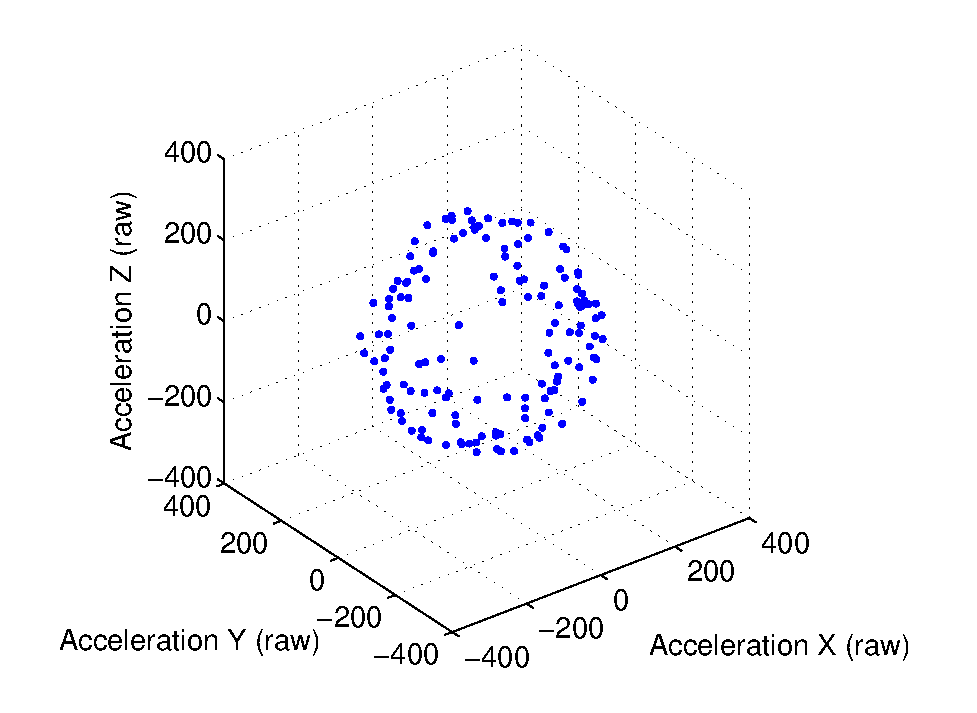
\includegraphics[width=0.7\textwidth]{figuras/Fundamentos/Fundamentos5EPS}
\caption{Representaci�n 3D de la aceleraci�n recogida durante las posiciones casi-est�ticas.}
\label{fig:Fundamentos5}
\end{figure}

Entonces alimentamos el algoritmo de minimizaci�n con esos datos y encontramos los par�metros de calibraci�n �ptimos. La ecuaci�n \ref{eq:14} muestra la estimaci�n de los par�metros de calibraci�n para el aceler�metro triaxial que se encuentra en el m�dulo de GaitWatch que se coloca en el tronco del paciente.

\begin{equation}
\label{eq:14}
\begin{bmatrix}
256.68 & -4.01 \cdot 10^{-5} & -2.41 \cdot 10^{-5} \\
-4.01 \cdot 10^{-5} & 262.74 & -3.98 \cdot 10^{-7} \\
-2.41 \cdot 10_{-5} & -3.98 \cdot 10^{-7} & 263.04
\end{bmatrix}
\end{equation}
\begin{displaymath}
\begin{bmatrix}
\mathbf{b}=-23.69 & -6.95 & 22.85
\end{bmatrix}
\end{displaymath}

La figura \ref{fig:Fundamentos6} muestra la aceleraci�n casi-est�tica calibrada. Observe como los puntos definen ahora una esfera centrada en el origen con un radio de 1(g). Posteriormente veremos como se calcula.

\begin{figure}[H]
\centering
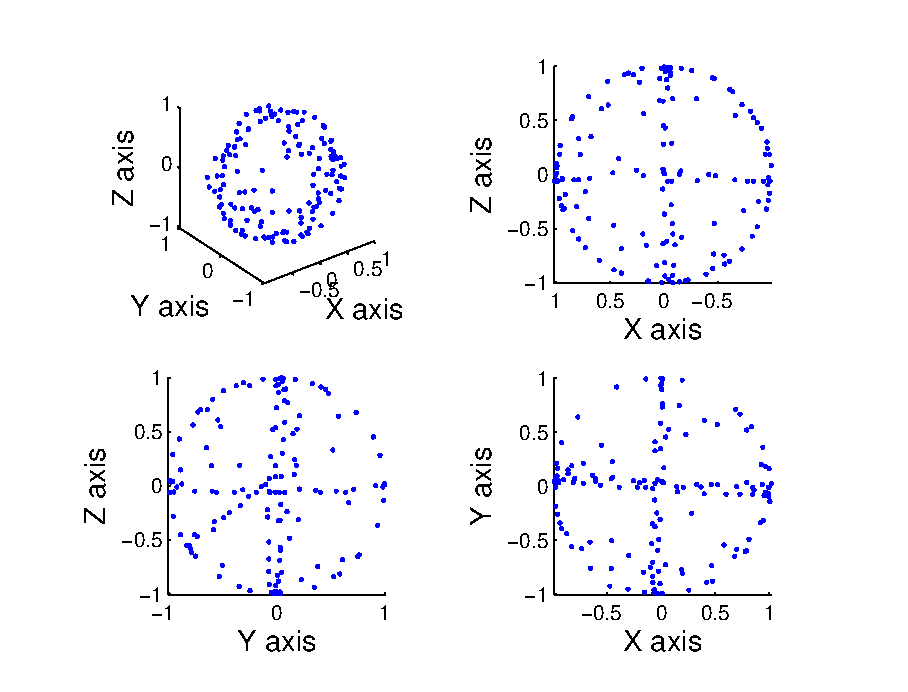
\includegraphics[width=0.7\textwidth]{figuras/Fundamentos/Fundamentos6EPS}
\caption{Representaci�n 3D de las posiciones casi-est�ticas calibradas}
\label{fig:Fundamentos6}
\end{figure}


 Los par�metros c�lculados anteriormente son incluidos a la siguiente ecuaci�n  que son utilizados para calibrar la aceleraci�n en bruto y transformarla a unidades f�sicas (la figura \ref{fig:Fundamentos6} nos mostraba los resultados), adem�s de paliar algunos de los errores no deseados presentes a la salida del sensor:
 
 
 

\begin{equation}
\mathbf{a}_{cal}=S^{-1}(\mathbf{a}_{raw}-\mathbf{b})
\end{equation}

donde $ \mathbf{a}_{cal}$ es un vector de tres dimensiones que contiene la aceleraci�n calibrada, S es la matriz de ortogonalidad calculada, $ \mathbf{a}_{raw} $ es el vector de tres dimensiones que contiene la aceleraci�n original y \textbf{b}  es el vector bias triaxial calculado.





Para el aceler�metro biaxial podemos adaptar los ya mencionados m�todos de dos dimensiones. Sin embargo, las maniobras de calibraci�n ser�an mucho m�s complicadas porque necesitar�amos bloquear la unidad incluyendo el aceler�metro  en el plano XZ y despu�s describir una rotaci�n lenta y completa para recoger las posiciones casi-est�ticas.

Optamos por llevar a cabo un procedimiento de calibraci�n de un solo eje que s�lo requiere recoger datos de dos posiciones en cada eje. Este procedimiento es muy simple; primero ponemos el eje deseado paralelo al vector gravedad  y lo dejamos en esa posici�n un par de segundos. Seguidamente, le damos la vuelta y lo colocamos de forma anti-paralela al vector de la gravedad donde lo volvemos a dejar est�tico otros dos segundos. Procediendo de esta manera, conocemos los valores originales que corresponden a +1g y -1g respectivamente. Ya que los aceler�metros incluidos en las unidades del GaitWatch son lineales, podemos entonces encontrar la ecuaci�n de calibraci�n en una forma muy simple. La ecuaci�n de calibraci�n est� definida como sigue,

\begin{equation}
a_{cal}=k \cdot a_{raw}+b
\end{equation}

donde $ a_{cal} $ es la aceleraci�n calibrada, $ a_{raw} $ es la aceleraci�n original, \textit{k} es el factor de escala y \textit{b} es el offset. Si sustituimos los dos valores recogidos tendr�amos el siguiente sistema de ecuaciones de donde es sencillo encontrar los valores de \textit{k} y \textit{b},

\begin{equation}
1=k \cdot a_{raw,+} + b
\end{equation}
\begin{displaymath}
-1=k \cdot a_{raw,-} + b
\end{displaymath}

donde $ a_{raw,+} $ y $ a_{raw,-} $ son las aceleraciones originales recogidas en las posiciones paralela y anti-paralela respectivamente.

Las unidades de GaitWatch situdadas en las espinillas y los muslos contienen un aceler�metro biaxial(X,Z) por lo tanto ponemos la unidad en las cuatro posiciones requeridas (dos en cada eje) y entonces aplicamos el detector de posiciones casi-est�ticas para extraer los valores en esas posiciones.

La figura \ref{fig:Fundamentos7} muestra la aceleraci�n original recogida en las cuatro posiciones y los valores casi-est�ticos estraidos para el aceler�metro en la espinilla izquierda.

Usando este procedimiento los par�metros de calibraci�n son encontrados en todas las unidades. La tabla \ref{tab:param_acc_biax} los muestra.

\begin{figure}[H]
\centering
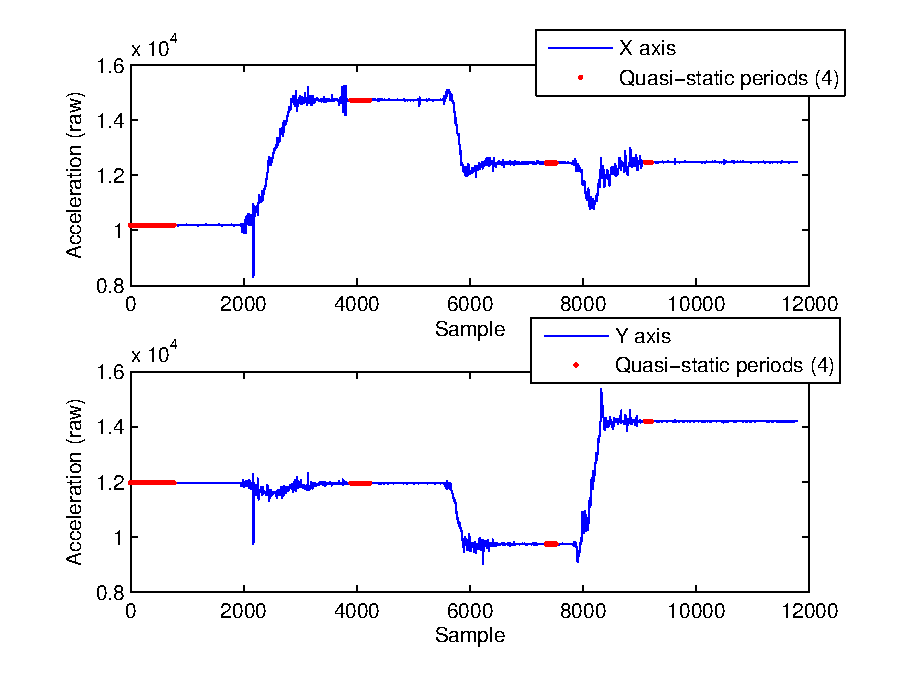
\includegraphics[width=0.6\textwidth]{figuras/Fundamentos/Fundamentos7EPS}
\caption{Aceleraci�n original recogida cuando ambos ejes X y Z son colocados paralelo y anti-paralelo al vector gravedad}
\label{fig:Fundamentos7}
\end{figure}

\begin{table}[h]
	\caption{Par�metros de calibraci�n de los aceler�metros biaxiales}	
	\centering
		\begin{tabular}{|c|c|c|c|}\hline
		\label{tab:param_acc_biax}
		Unidad 				& Eje 	& Factor de escala 	& Sesgo 	\\ \hline
		Espinilla izquierda & X			& 4.45e-04									& -5.59					\\
		Espinilla izquierda	& Z			& 4.49e-04									& -5.36					\\
		Muslo izquierdo & X			& 4.58e-04									& -5.76					\\
		Muslo izquierdo	& Z			& 4.74e-04									& -5.70					\\
		Espinilla derecha  & X			& 4.38e-04									& -5.50					\\
		Espinilla derecha	& Z			& 4.77e-04									& -5.72					\\
		Muslo derecho  & X			& 4.36e-04									& -5.44				\\
		Muslo derecho	& Z			& 4.43e-04									& -5.34				\\ \hline
		
		\end{tabular}
		
		
\end{table}


\subsubsection{Calibraci�n del magnet�metro}

La calibraci�n de un magnet�metro triaxial est� tambi�n basada en el algoritmo de Camps et al. usado para la calibraci�n del aceler�metro. En este caso, solo necesitamos cambiar los datos recogidos en las maniobras y el valor de la magnitud del vector de referencia (que en este caso es el vector de campo magn�tico de la Tierra).

Las maniobras en este caso son m�s simples porque el magnet�metro no se ve afectado por la aceleraci�n lineal. Por lo tanto, podemos mover libremente el magnet�metro 


\begin{figure}[H]
\centering
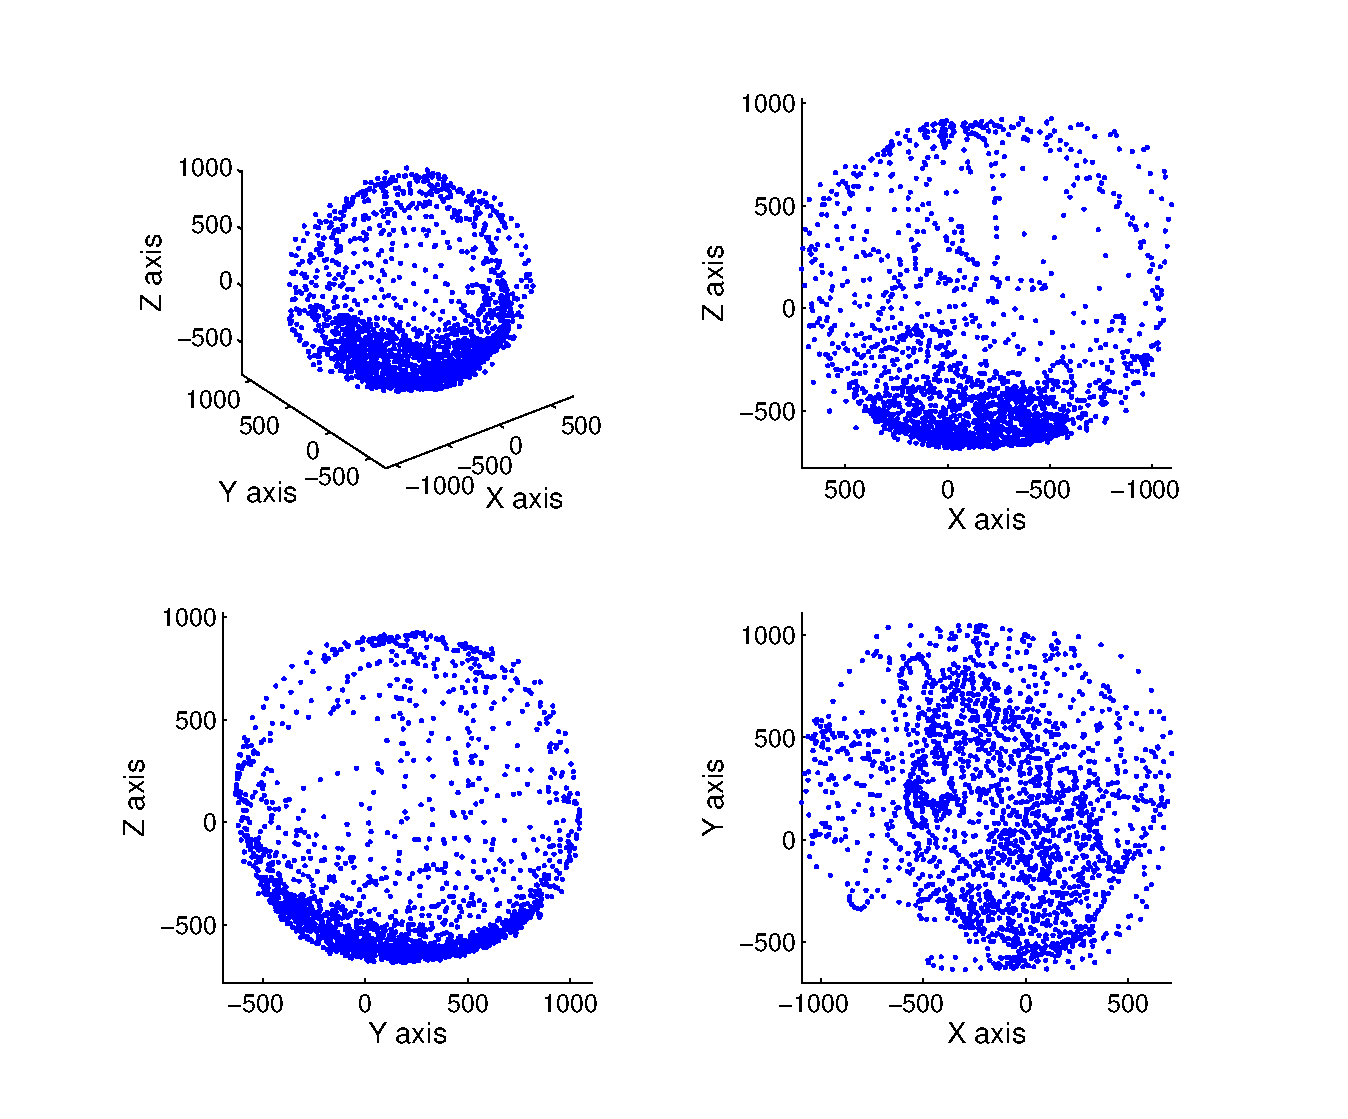
\includegraphics[width=0.65\textwidth]{figuras/Fundamentos/Fundamentos8EPS}
\caption{Campo magn�tico original recogido por el movimiento aleatorio del la unidad del tronco que contiene el magnet�metro}
\label{fig:Fundamentos8}
\end{figure}


a cualquier velocidad intentando cubrir el mayor espacio posible. La figura \ref{fig:Fundamentos8} muestra la representaci�n 3D del campo magn�tico original medido llevando a cabo esas maniobras.

Idealmente, esos datos deben de describir una esfera centrada en el origen con un radio dado por la magnitud del campo magn�tico local de la Tierra. Al comprobar el campo magn�tico en la calculadora del American National Geophysical Data Center, obtenemos el valor para Munich (lugar donde fueron realizadas las maniobras de calibraci�n), que es de 0.482352 Gauss. Entonces proporcionamos al algoritmo \cite{funda13} los datos mostrados en la figura \ref{fig:Fundamentos8} y los par�metros de calibraci�n son calculados. An�logamente al aceler�metro, el campo magn�tico calibrado es encontrado aplicando la siguiente ecuaci�n,


\begin{equation}
\mathbf{h}_{cal}=S^{-1}(\mathbf{h}_{raw}-\mathbf{b})
\end{equation}

donde otra vez $ \mathbf{h}_{cal} $ es un vector tridimensional que contiene el campo magn�tico calibrado, S es la matriz de ortogonalidad calculada, $ \mathbf{h}_{raw} $ es el vector de tres dimensiones que contiene el campo magn�tico original y \textbf{b} es el vector bias triaxial calculado. Si aplicamos esta ecuaci�n a los valores originales usados para calcular los par�metros de calibraci�n, podemos ver como ahora definen una esfera centrada en 0 y con un radio de 0.482352 Gauss (figura \ref{fig:Fundamentos9})


\begin{figure}[H]
\centering
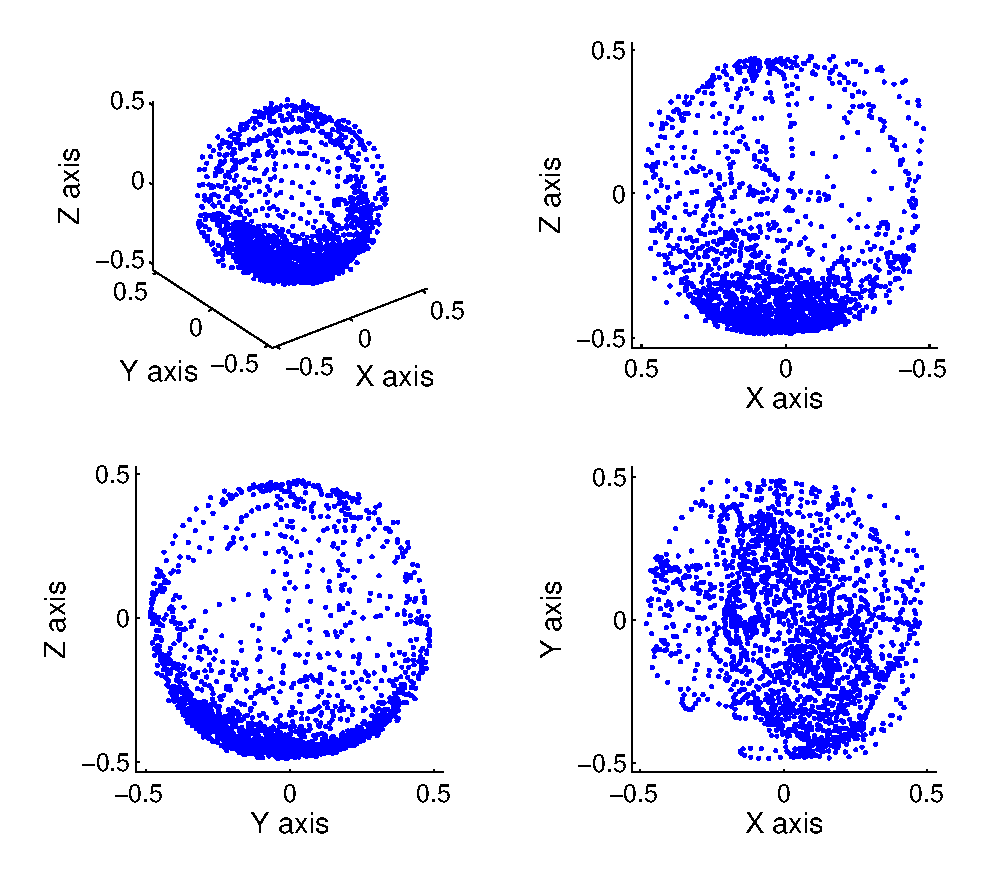
\includegraphics[width=0.6\textwidth]{figuras/Fundamentos/Fundamentos9EPS}
\caption{Campo magn�tico calibrado recogido moviendo aleatoreamente la unidad del tronco que contiene el magnet�metro.}
\label{fig:Fundamentos9}
\end{figure}

La figura \ref{fig:Fundamentos10} muestra las se�ales originales y calibradas para los tres ejes del magnet�metro incluidos en la unidad del tronco.

\begin{figure}[H]
\centering
\includegraphics[width=0.6\textwidth]{figuras/Fundamentos/Fundamentos10EPS}
\caption{Campo magn�tico original (izquierda) vs. Campo magn�tico calibrado (derecha) recogidos con movimientos aleatorios de la unidad del tronco que contiene el magnet�metro}
\label{fig:Fundamentos10}
\end{figure}


Los par�metros de calibraci�n  del magnet�metro en la unidad del tronco se enumeran a continuaci�n

\begin{equation}
S=
\begin{bmatrix}
1.75 \cdot 10^{3} & -3.46 \cdot 10^{-8} & -3.04 \cdot 10^{-6} \\
 -3.46 \cdot 10^{-8} & 1.97 \cdot 10^{3} & 1.42 \cdot 10^{-5} \\
 -3.04 \cdot 10^{-5} & 1.42 \cdot 10^{-6} & 1.83 \cdot 10^{3}
\end{bmatrix}
\end{equation}
\begin{displaymath}
\mathbf{b}=
\begin{bmatrix}
14.84 & 102.43 & -42.04
\end{bmatrix}
\end{displaymath}

\subsubsection{Calibraci�n del gir�scopo}

El gir�scopo es el �ltimo tipo de sensor que queda por ser calibrado. La forma m�s precisa para calibrar un gir�scopo es someterlo a diferentes rotaciones conocidas sus velocidades y luego asociarlos a los valores originales recogidos para obtener la ecuaci�n de calibraci�n. Si no tenemos mesa de rotaci�n de velocidad variable, podemos usar un equipo m�s sencillo y sujetar el someter al gir�scopo a rotaciones conocidas en lugar de velocidades angulares conocidas. Para calibrar cada uno de los ejes necesitamos construir un dispositivo parecido al que se muestra en la figura \ref{fig:Fundamentos11}. Este dispositivo debe permitir la rotaci�n de la unidad que contiene el gir�scopo alrededor de 180� (otras configuraciones del dispositivo que permiten diferentes rotaciones conocidas tambi�n son v�lidas).

\begin{figure}[H]
\centering
\includegraphics[width=0.7\textwidth]{figuras/Fundamentos/Fundamentos11}
\caption{Dispositivo de calibraci�n del gir�scopo}
\label{fig:Fundamentos11}
\end{figure}

Una vez que el dispositivo de calibraci�n est� listo, las maniobras de calibraci�n no son complicadas. Cada una de las unidades debe estar adheridas a la superficie del dispositivo y entonces necesitamos llevar a cabo la rotaci�n completa de 180� una serie de veces para posteriormente promediar los datos calculados. 

Para calcular los par�metros de calibraci�n vamos a utilizar el hecho de que la integraci�n de la velocidad angular conduce a un desplazamiento angular. Por lo tanto, si sometemos al gir�scopo a una rotaci�n conocida (180� en este caso), podemos aplicar las siguientes ecuaciones para encontrar el factor de escala,

\begin{equation}
\mu_{raw}=k.\omega+b
\end{equation}
\begin{equation}
\label{eq:21}
\omega=\frac{\mu_{raw}-b}{k}
\end{equation}
\begin{equation}
\mu_{raw,corr}=\mu_{raw}-b
\end{equation}
\begin{equation}
\int \omega dt=\frac{\int \mu_{raw,corr}dt}{k}
\end{equation}
\begin{equation}
\Omega=\int \omega dt
\end{equation}
\begin{equation}
\theta=\int \mu_{raw,corr}dt
\end{equation}
\begin{equation}
\Omega=\frac{\theta}{k}
\end{equation}
\begin{equation}
k=\frac{\theta}{\Omega}
\end{equation}

donde $ u_{raw} $ es la velocidad angular original recogida, $ \omega $ es la velocidad angular real (en unidades f�sicas), \textit{k} es el factor de escala y \textit{b} es el offset. En este caso $ \Omega=180 � $ y $ \theta $ es la velocidad angular original integrada (corregida en offset) durante la rotaci�n de 180�. Podemos ver que antes de la integraci�n de la velocidad angular necesitamos sustraer el offset.

El offset se encuentra f�cilmente dejando las unidades en una posici�n est�tica antes de empezar la rotaci�n. Para tener en cuenta los efectos del ruido, calculamos la moda de todas las muestras recogidas mientras los sensores estaban est�ticos.

Desde el punto de vista pr�ctico, la rutina de calibraci�n de Matlab muestra por primera vez la se�al de la velocidad angular original recogida y pide al usuario seleccionar los puntos inicial y final del per�odo est�tico como muestra la figura \ref{fig:Fundamentos12}.

Una vez encontrado el offset, necesitamos indicarle a la rutina cada uno de los puntos de inicio y final de las rotaciones, as� sabremos los instantes inicial y final de la integraci�n. Para lograrlo utilizaremos la herramienta \textit{datacursor} de Matlab. Es importante seleccionar �nicamente las rotaciones positivas (como se indica en la figura \ref{fig:Fundamentos13}), es decir, cuando la velocidad angular incrementa  y despu�s decrementa. La rutina entonces integrar� los segmentos seleccionados de la se�al y promediar� el factor de escala de cada uno de ellos.


\vspace{1cm}
La calibraci�n de la velocidad angular es finalmente encontrada sustiyendo los par�metros de calibraci�n calculados en la ecuaci�n \ref{eq:21}.


 \vspace{-28mm}
\begin{figure}[H]
\centering
\includegraphics[width=1.0\textwidth]{figuras/Fundamentos/Fundamentos12EPS}
\caption{Rutina de calibraci�n del gir�scopo: selecci�n del per�odo para calcular el offset.}
\label{fig:Fundamentos12}
\end{figure}


\begin{figure}[H]
\centering
\includegraphics[width=1.0\textwidth]{figuras/Fundamentos/Fundamentos13EPS}
\caption{Rutina de calibraci�n del gir�scopo: selecci�n de las rotaciones positivas para el c�lculo del factor de escala}
\label{fig:Fundamentos13}
\end{figure}

La Tabla \ref{tab:par_cali_giro} enumera los par�metros de calibraci�n calculados para todos los gir�scopos del GaitWatch. 


\begin{table}[h]
	\caption{Par�metros de calibraci�n de los gir�scopos}	
	\centering
		\begin{tabular}{|c|c|c|c|}\hline
		\label{tab:par_cali_giro}
		Unidad 				& Eje 	& Factor de escala 	& Sesgo 	\\ \hline
		Espinilla izquierda & Y			& -5.84									& 11591					\\
		Muslo izquierdo	& Y			& -6.36									& 11720					\\
		Espinilla derecha & Y			& -5.95									& 11618					\\
		Muslo derecho	& Y			& -6.40									& 11740					\\
		Brazo izquierdo  & X			& -5.89									& 12087					\\
		Brazo izquierdo	& Y			& 5.75									& 10937				\\
		Brazo derecho  & X			& -6.02									& 11543			\\
		Brazo derecho	& Y			& 5.64									& 11415		\\ 
		Tronco  & X			& -16.15									& -10				\\
		Tronco  & Y			& 16.02									& 62				\\
		Tronco  & Z			& 16.23									& 31				\\ \hline
		\end{tabular}
		
		
\end{table}


\subsubsection{Recapitulaci�n}

Como resumen final, una vez que todos los par�metros de calibraci�n de todos los sensores est�n calculados, s�lo necesitamos aplicar las siguientes ecuaciones,

\begin{itemize}
\item \textbf{Aceler�metro}:

	\begin{itemize}
	\item Aceler�metro triaxial:
	\begin{equation}
	\mathbf{a}_{cal}=S^{-1}(\mathbf{a}_{raw}-\mathbf{b})
	\end{equation}
	\item Aceler�metro biaxial:
	\begin{equation}
	a_{cal}=k \cdot a_{raw}+b
	\end{equation}
	\end{itemize}

\item \textbf{Magnet�metro}:
\begin{equation}
\mathbf{h}_{cal}=S^{-1}(\mathbf{h}_{raw}-\mathbf{b})
\end{equation}

\item \textbf{Gir�scopo}:
\begin{equation}
\omega_{cal}=\frac{u_{raw}-b}{k}
\end{equation}
\end{itemize}

\subsection{C�lculo de orientaci�n}


Esta subsecci�n comienza con una introducci�n a los conceptos que ser�n usados a lo largo del la misma, posteriormente se continuar�  describiendo los algoritmos utilizados en el c�lculo de orientaci�n para el sistema GaitWatch. No es necesario explicar la parte acociada al dispositivo ECnsole ya que los algoritmos aplicados son id�nticos (vuelve a ocurrrir lo mismo que en la parte de calibraci�n).

A continuac�on se enumeran a modo de resumen los algoritmos de c�lculo de orientaci�n com�n a los dos dispositivos:

\begin{itemize}
\item Integraci�n de la velocidad angular.
\item Descomposici�n de la gravedad.
\item El Filtro de Kalman.
\item El Filtro de Kalman Extendido.
\end{itemize}

De forma equivalente al proceso de calibraci�n, las pautas para llevar a cabo el proceso de c�lculo de los algoritmos de orientaci�n vienen recogidas en \cite{funda5} donde se realiza una descripci�n m�s minuciosa del procedimiento.


\subsubsection{Conceptos b�sicos}

\paragraph{Sistemas de coordenadas \\ \\}


 Un sistema de coordenadas no es m�s que un conjunto de vectores y n�meros sin 
sentido. Para que estos valores adquieran significado, es necesario relacionarlos 
con una referencia conocida. A continuaci�n definiremos los principales sistemas de coordenadas son recogidos en \cite{funda23}como sigue,



\begin{itemize}
\item \textbf{El sistema de coordenadas inercial (i-frame).} Este sistema de coordenadas tiene su origen en el centro de masas de la Tierra y se 
supone que no rota respecto al espacio inercial, ya que se mueve con el planeta. 
Sabemos que eso no es del todo cierto, porque la Tierra gira con respecto al Sol y 
adem�s de su propia rotaci�n $ \Omega $ , pero se tomar� este sistema como inercial.

Los ejes del sistema ECI est�n fijados en las estrellas: El eje Z coincide con el eje 
polar y el plano perpendicular al eje Z coincide con el Ecuador. El eje X e Y no 
rotan con la tierra, apuntando X directamente al equinoccio Vernal.

\item \textbf{El sistema de coordenadas de Navegaci�n (n-frame).}Tiene su origen en la localizaci�n del sistema inercial (longitud latitud). Es un 
sistema local con sus ejes X Y en el plano tangente al punto de la Tierra donde est� 
el origen. T�picamente el eje X apuntar� al norte, ele eje Y al Este y el eje Z abajo, 
aunque debe ser especificado.
Tambi�n se le conoce como NED (North, East, Down) ya que sus ejes apuntan a 
estas direcciones. Otra posible configuraci�n, ser�a con el eje X apuntando al este, el eje Y apuntando al norte y el 
eje Z apuntando hacia arriba, tambi�n conocido como ENU (East, North, Up). La figura \ref{fig:Fundamentos28} representa el esquema de coordenas de navegaci�n ENU. 
\begin{figure}[H]
\centering
\includegraphics[width=0.4\textwidth]{figuras/Fundamentos/Fundamentos28}
\caption{Esquema de coordenadas de navegaci�n ENU \cite{funda22}.}
\label{fig:Fundamentos28}
\end{figure}
\item \textbf{El sistema de coordenadas Body (b-frame).} Este sistema tiene su origen en el centro de masas del vehiculo. T�picamente usado 
en plataformas Strapdown, es decir, cuando los sensores tienen tambi�n como 
centro de masas el vehiculo y sus ejes se mueven con �l. La figura \ref{fig:Fundamentos27} nos muestra este sistema de cooordenadas.

\begin{figure}[H]
\centering
\includegraphics[width=0.6\textwidth]{figuras/Fundamentos/Fundamentos27}
\caption{Esquema de coordenadas de Body en un veh�culo \cite{funda23}.}
\label{fig:Fundamentos27}
\end{figure}


\end{itemize} 


\paragraph{Representaci�n de la posici�n}

\subparagraph{�ngulos de Euler \\ \\}

Otro m�todo bastante popular para especificar la orientaci�n angular de un sistema 
de coordenadas respecto a otro es el uso de los tres �ngulos de Euler. Tres �ngulos, 
que mediante una sucesi�n ordenada de giros, definen el cambio de un sistema de 
coordenadas a otro. En este caso, utilizar�amos como referencia \textit{el sistema de coordenadas de navegaci�n inercial}.

Los tres �ngulos de Euler son definidos en \cite{funda5} como sigue,

\begin{itemize}
\item El �ngulo \textit{roll} ($ \Phi $) determina la rotaci�n alrededor del eje X. Est� normalmente acotado en el intervalo ($ -\pi $,$ \pi $].
\item El �ngulo \textit{pitch} ($ \theta $) determina la rotaci�n alrededor del eje Y. Est� normalmente acotado en el intervalo [$ \frac{-\pi}{2} $,$ \frac{\pi}{2} $].
\item El �ngulo \textit{yaw} ($ \psi $) determina la rotaci�n alrededor del eje Z. Est� normalmente acotado en el intervalo ($ -\pi $,$ \pi $].
\end{itemize}

La figura \ref{fig:Fundamentos29} representa los �ngulos de Euler:

\begin{figure}[H]
\centering
\includegraphics[width=0.6\textwidth]{figuras/Fundamentos/Fundamentos29}
\caption{Representaci�n bidimensional de los giros en roll, pitch y yaw \cite{funda23}.}
\label{fig:Fundamentos29}
\end{figure}

\paragraph{Matrices de rotaci�n \\ \\}

Las matrices de rotaci�n \cite{funda5} son utilizadas para llevar a cabo rotaciones en el espacio Eucl�deo. De esta manera se usar�n las matrices para poder mapear las rotaciones de Euler en el interior de las matrices. As�, si multiplicamos un vector por la matriz de rotaci�n obtendremos su versi�n rotada en el espacio.

\begin{equation}
\mathbf{v'}=R\mathbf{v}
\end{equation}

La obtenci�n de las matrices implica una serie de operaciones trigonom�tricas. A continuaci�n vamos a ir viendo cada uno de los giros por separado (asumiendo que estamos usando el sistema de coordenadas NED). Finalmente se obtendr� la matriz de rotaci�n como resultado de la multiplicaci�n de las tres  matrices de giro.

\textbf{Giro en Yaw}

Es el primero de los giros que se har�. Con esta matriz de cambio se puede pasar 
del sistema de coordenadas (X, Y, Z) al nuevo sistema 
\begin{math}
(X', Y', Z')
\end{math}.


\begin{equation}
C_{\psi}=
\begin{bmatrix}
\cos\psi & \sin\psi & 0 \\
-\sin\psi & \cos\psi & 0\\
0 & 0 & 1
\end{bmatrix}
\end{equation}


\textbf{Giro en Pitch}

Giramos el sistema \begin{math}
(X',Y',Z')
\end{math} para conseguir 
\begin{math}
(X'',Y'',Z'')
\end{math} 



\begin{equation}
C_{\theta}=
\begin{bmatrix}
\cos\theta & 0 & -\sin\theta \\
0 & 1 & 0\\
\sin\theta & 0 & \cos\theta
\end{bmatrix}
\end{equation}


\textbf{Giro en Roll}

El �ltimo de los giros: de \begin{math}
(X'',Y'',Z'')
\end{math} a
\begin{math}
(x,y,z)
\end{math} 



\begin{equation}
C_{\Phi}=
\begin{bmatrix}
1 & 0 & 0 \\
0 & \cos\Phi & \sin\Phi\\
0 & -\sin\Phi & \cos\Phi
\end{bmatrix}
\end{equation}


Entonces, definimos la matriz de cambio de coordenadas $ C_{n}^{b} $
as�:

\begin{equation}
C_{n}^{b}=C_{\psi}C_{\theta}C_{\Phi}
\end{equation}

\begin{equation}
\label{ecuacion:37}
C_{n}^{b}=
\begin{bmatrix}
\cos\theta\cos\psi & cos\theta\sin\psi & -\sin\theta \\
\sin\phi\sin\theta\cos\phi-\cos\phi\sin\psi& \sin\phi\sin\theta\sin\psi+\cos\phi\cos\psi & \sin\phi\cos\theta\\
\cos\phi\sin\theta\cos\psi+\sin\phi\sin\psi& \cos\phi\sin\theta\sin\psi-\sin\phi\cos\psi & \cos\phi\cos\theta
\end{bmatrix}
\end{equation}


La ecuaci�n \ref{ecuacion:37} corresponde a la matriz de cambio de coordenadas de navegaci�n a \textit{body}. Si quisieramos la transformaci�n inversa, es decir, cambio de \textit{body} a navegaci�n se obtiene aplicando

\begin{equation}
C^{n}_{b}=(C^{b}_{n})^{-1}=(C^{b}_{n})^{T}
\end{equation}

que conduce a

\begin{equation}
C^{n}_{b}=
\begin{bmatrix}
\cos\theta\cos\psi&\sin\phi\sin\theta\cos\phi-\cos\phi\sin\psi&\cos\phi\sin\theta\cos\psi+\sin\phi\sin\psi \\
cos\theta\sin\psi&\sin\phi\sin\theta\sin\psi+\cos\phi\cos\psi&\cos\phi\sin\theta\sin\psi-\sin\phi\cos\psi  \\
-\sin\theta&\sin\phi\cos\theta&\cos\phi\cos\theta
\end{bmatrix}
\end{equation}

\vspace{1cm}

\paragraph{Cuaterniones \\ \\ \\}



Los cuaterniones \cite{funda5} (tambi�n llamados cuaternios) son una extensi�n de los n�meros reales, similar a la de los n�meros complejos. Mientras que los n�meros complejos son una extensi�n de los reales por la adici�n de la unidad imaginaria i, tal que $ i*i=-1 $, los cuaterniones son una extensi�n generada de manera an�loga a�adiendo las unidades imaginarias: i, j y k a los n�meros reales y tal que $ i^{2}=j^{2}=k^{2}=ijk=-1 $.




\textbf{�C�mo est� compuesto un cuaterni�n?}

Un cuaterni�n es un n�mero definido de la siguiente manera:

\begin{equation}
q=a+bi+cj+dk
\end{equation}


donde a,b,c y d son n�meros reales arbitrarios. Normalmente, a es un escalar  y  $ bi+cj+dk $ es el vector del cuaterni�n. No podemos pensar que (a,b,c) como un vector t�pico en 3D, es un vector en 4D, aunque es muy poco intuitivo de ver.


Existen otras representaciones para los cuaterniones y se van a mostrar a continuaci�n:

\begin{equation}
\mathbf{q}=(a,b,c,d)=[a,(b,c,d)]=(q_{0},q_{1},q_{2},q_{3})
\end{equation}

Adem�s, vamos a resaltar los elementos neutros o elemento identidad para las operaciones suma y resta:

\begin{math}
\mathbf{q}=[1,(0,0,0)] .
\end{math}
es el cuaterni�n identidad para la multiplicaci�n

\begin{math}
\mathbf{q}=[0,(0,0,0)] 
\end{math}
es el cuaterni�n identidad para la suma.


\vspace{1.5cm}

\textbf{Cuaterniones y las rotaciones}

Un cuaterni�n \cite{funda24} es una forma alternativa de representar rotaciones a trav�s del cualquier eje. Comparados con los �ngulos de Euler, son m�s simples de componer y evitan el problema del bloqueo del card�n (es la p�rdida de un grado de libertad que ocurre cuando 2 de los 3 ejes necesarios para las rotaciones en 3D, son llevados a la misma direcci�n). Comparados con las matrices de rotaci�n, son m�s eficientes y m�s estables num�ricamente. El elemento utilizado son los cuaterniones unitarios y son aquellos que cumplen que

\begin{equation}
a^{2}+b^{2}+c^{2}+d^{2}=1
\end{equation} 

Los cuaterniones unitarios son especiales porque representan la orientaci�n en el espacio 3D (permiten representar rotaciones en 3D de manera muy sencilla). Si \textbf{q} es un cuaterni�n unitario, �ste puede pensarse como una esfera de radio 1 en el espacio 4D, aunque resulte poco intuitivo de ver. A trav�s de la figura \ref{fig:Fundamentos30} nos podemos hacer una idea.


\begin{figure}[H]
\centering
\includegraphics[width=0.4\textwidth]{figuras/Fundamentos/Fundamentos30}
\caption{Representaci�n en el espacio de un cuaterni�n unitario \cite{funda24}.}
\label{fig:Fundamentos30}
\end{figure}

donde \begin{math}
\mathbf{q}=[\cos\frac{\theta}{2} + \sin\frac{\theta}{2}\vec{\mathbf{v}}]
\end{math}

con

\begin{math}
\|\vec{\mathbf{v}}\|=1
\end{math}


\vspace{1cm}
As�, una rotaci�n se puede representar con el cuaterni�n
\begin{math}
\mathbf{q}=(a,(b,c,d))
\end{math}
, donde $ (b,c,d) $ es el eje de rotaci�n y a es el valor del �ngulo de rotaci�n.

\vspace{1cm}

\textbf{Conversi�n desde cuaterniones}

Para usar los cuaterniones en la orientaci�n, es necesario convertirlos a otras representaciones (como matrices) y volverlos a cuaterniones.

\begin{itemize}
\item De cuaterni�n a matriz.

\begin{math}
\mathbf{q}=(q_{0},q_{1},q_{2},q_{3})
\end{math}
equivale a

\begin{equation}
M=
\begin{bmatrix}
q_{0}^{2}+q_{1}^{2}-q_{2}^{2}-q_{3}^{2} & 2q_{1}q_{2}-2q_{0}q_{3} & 2q_{1}q_{3}+2q_{0}q_{2} \\
2q_{1}q_{2}+2q_{0}q_{3} & q_{0}^{2}-q_{1}^{2}+q_{2}^{2}-q_{3}^{2}& 2q_{2}q_{3}-2q_{0}q_{1} \\
2q_{1}q_{3}-2q_{0}q_{2} & 2q_{2}q_{3}+2q_{0}q_{1} & q_{0}^{2}-q_{1}^{2}-q_{2}^{2}+q_{3}^{2}
\end{bmatrix}
\end{equation}

\vspace{1cm}
\item De cuaterni�n a ejes/�ngulo.

\begin{math}
\mathbf{q}=(q_{0},q_{1},q_{2},q_{3})
\end{math}
equivale a

\begin{equation}
\Theta=2\cos (q_{0})/s
\end{equation}
\begin{equation}
V=(q_{1},q_{2},q_{3})/s
\end{equation}

donde
\begin{math}
s=\sqrt{q_{1}^{2}+q_{2}^{2}+q_{3}^{2}}
\end{math}

\vspace{1cm}

\item De cuaterni�n a �ngulos de Euler.


\begin{math}
\mathbf{q}=(q_{0},q_{1},q_{2},q_{3})
\end{math}
equivale a


\begin{equation}
\label{ecuacion:46}
\phi=\arctan\left(\dfrac{2(q_{0}q_{1}+q_{2}q_{3})}{1-2(q_{1}^{2}+q_{2}^{2})}\right)
\end{equation}

\begin{equation}
\label{ecuacion:47}
\theta=\arcsin\left(2(q_{0}q_{2}-q_{3}q_{1})\right)
\end{equation}

\begin{equation}
\label{ecuacion:48}
\psi=\arctan\left(\dfrac{2(q_{0}q_{3}+q_{1}q_{2})}{1-2(q_{2}^{2}+q_{3}^{2})}\right)
\end{equation}


Puesto que arctan y arcsin son funciones cuyo resultado se mueve en el intervalo $ [-\pi/2,\pi/2] $, no podemos definir todas las posibles orientaciones teniendo tres rotaciones con con dicho intervalo. Como antes mencionamos, para cubrir todas las posibles orientaciones, roll($ \phi $) y yaw($ \psi $) est�n generalmente definidos dentro de un rango $ (-\pi,\pi] $ mientras pitch$ (\theta) $ est� delimitado entre $ [-\pi/2,\pi/2] $. Por lo tanto, para definir todas las posibles posiciones y rotaciones de un cuerpo en las tres dimensiones del espacio necesitamos sustituir la funci�n arctan en \ref{ecuacion:46} y \ref{ecuacion:48} por la funci�n atan2 que est� definida en el intervalo $ (-\pi,\pi] $.

\end{itemize}


\textbf{Conversi�n a cuaterniones}

\begin{itemize}
\item De ejes/�ngulo a cuaterniones.

\begin{math}
\Theta,V
\end{math}
equivale a

\begin{equation}
\mathbf{q}=(\cos(\Theta/2),u_{x}\sin(\Theta/2),u_{y}\sin(\Theta/2),u_{z}\sin(\Theta/2))
\end{equation}

donde $ \mathbf{u}=(u_{x},u_{y},u_{z}) $ es un vector en $ \mathbb{R}^{3} $ de magnitud igual a la unidad.

\vspace{1cm}

\item De �ngulos de Euler a cuaterni�n.

Sea $ (\phi,\theta,\psi) $ hay que obtener 3 cuaterniones independientes

\begin{equation}
q_{\phi}=[\cos(\phi/2),\sin(\phi/2),0,0]
\end{equation}

\begin{equation}
q_{\theta}=[\cos(\theta/2),0,\sin(\theta/2),0]
\end{equation}

\begin{equation}
q_{\psi}=[\cos(\psi/2),0,0,\sin(\psi/2)]
\end{equation}

\end{itemize}

\vspace{1.5cm}

\subsubsection{C�lculo de la orientaci�n usando los �ngulos de Euler}




\paragraph{Integraci�n de la velocidad angular} ~\\


El gir�scopo mide la velocidad angular alrededor de cada uno de los ejes Cartesianos relativa a su sistema corporal. Dicha velocidad angular puede ser integrada para estimar la rotaci�n del �ngulo entre los instantes $ t_0 $ a $ t_1 $. Por lo tanto, nosotros podemos calcular la posici�n del cuerpo relativa al marco de navegaci�n si, y solo si, la orientaci�n inicial del sistema corporal es conocida respecto al marco de navegaci�n. Una sencilla soluci�n es usar la aproximaci�n basada en la proyecci�n de la gravedad y los vectores del campo magn�tico de la tierra para calcular tal orientaci�n inicial cuando el cuerpo est� parado. 

Existen muchos m�todos num�ricos que pueden ser usados para integrar la velocidad angular. En este caso nosotros usaremos la integraci�n num�rica basada en la regla trapezoidal que calcula el �rea debajo de la funci�n realizando una aproximaci�n trapezoidal como sigue:


\begin{equation}
\alpha(n)=\alpha_{0}+\dfrac{T}{2}\sum_{k=1}^{n}[\omega_{g}(k)+\omega_{g}(k-1)]
\end{equation}


Donde \textit{T} es el per�odo de muestreo, \textit{n} es el n�mero de muestras, \textit{$ w_{g} $} la medida del gir�scopo en el instante \textit{n} y \textit{$ \alpha_{0} $} el �ngulo cuando \textit{n}=0. El �ngulo puede ser calculado tambi�n de forma recursiva usando

\begin{equation}
	\alpha(n)=\alpha(n-1)+\dfrac{T}{2}[\omega_{g}(n)+\omega_{g}(n-1)]
\end{equation}


donde $\alpha$(0)=$ \alpha_{0}$.

La ventaja principal de este m�todo es que una vez se conoce la orientaci�n inicial,

\begin{figure}[H]
	  \centering
	  \includegraphics[width=0.7\textwidth]{figuras/Fundamentos/Fundamentos1EPS}
	  \caption{Efectos del offset din�mico en la salida integrada de la se�al del gir�scopo}
	  \label{fig:Fundamentos1}
\end{figure}


puede ser usado para movimientos de baja intensidad o de alta intensidad mientras las medidas del gir�scopo no est�n afectadas por la aceleraci�n lineal. Sin embargo, la integraci�n del ruido y el offset din�mico conducen a un desplazamiento que crece r�pidamente que tiene efectos cr�ticos en el c�lculo del �ngulo de orientaici�n. Este efecto hace que la estimaci�n se absulatamente err�nea despu�s de unos pocos segundos como se puede ver en la figura \ref{fig:Fundamentos1}. 

Por tanto, el uso individual de la velocidad angular para el c�lculo de la orientaci�n es inviable si se usan gir�scopos MEMS los cuales presentan gran cantidad de ruido en los datos medidos. 



\paragraph{Descomposici�n de la gravedad}~\\


Podemos usar la proyecci�n del vector gravedad de la Tierra sobre los ejes del aceler�metro para estimar el �ngulo de orientaci�n de la estructura corporal respecto al marco de referencia. En el caso de GaitWatch, para las unidades del muslo y las espinillas s�lo est� disponible un aceler�metro biaxial. Por lo tanto, s�lo podemos calcular uno de los dos �ngulos de orientaci�n (roll y pitch) que pueden ser estimados por medio de estas t�cnica. Ya que estamos principalmente interesados en el �ngulo definido en el plano XZ, esto es, el �ngulo alrededor del eje  es decir, el pitch. El c�lculo de pitch s�lo puede ser v�lido si el �ngulo roll de las piernas tiende a 0. Debido a que las piernas se mueven principalmente en el plano sagital durante la marcha, consideraremos la siguiente expresi�n v�lida para el c�lculo del �ngulo pitch, 

	\begin{equation}
	\theta_{k}=atan2(a_{z,k},a_{x,k})
	\end{equation}

donde atan2 es la funci�n arcotangente con correcci�n de cuadrante.



\paragraph{Fusi�n de la velocidad angular con el �ngulo de orientaci�n calculado con el aceler�metro}~\\



\subparagraph{El filtro de Kalman} ~\\

El filtro de Kalman, es un conjunto de ecuaciones matem�ticas que proporciona un medio para estimar el estado de un proceso minimizando el error cuadr�tico medio.


Si se considera un modelo de tiempo lineal, invariante y continuo:

\begin{equation}
\mathbf{\dot{x}}(t)=F\mathbf{x}(t)+C\mathbf{u}(t)+I_{n}\mathbf{w}(t)
\end{equation}
\begin{displaymath}
\mathbf{z}(t)=H\mathbf{x}(t)+I_{q}\mathbf{v}(t)
\end{displaymath}

donde,


\begin{itemize}
	\item el operador  $ \mathbf{\dot x} $ denota la primera derivada \textbf{x}. 
	\item \textbf{x}(t) $ \epsilon $ $ \mathbb{R}^n $ es el estado (n$ \times 1 $) del vector incluyendo los n estados de las variables que describe el sistema.
	\item \textbf{z}(t) $ \epsilon $ $ \mathbb{R}^q $ es la salida (q$ \times 1 $) del vector incluyendo las observaciones (medidas) reales de los estados de las variables del proceso.
	\item \textbf{u}(t) $ \epsilon $ $ \mathbb{R}^p $ es el  (q$ \times 1 $) vector de control incluyendo las p entradas de las se�ales de control.
	\item F es el (n$ \times n $) estado de la matriz de transici�n.
	\item C es la (n$ \times p $) matriz de entrada.
	\item H es la (q$ \times n $)  matriz de salida.
	\item $ I_{n} $ es la (n$ \times n $) matriz identidad.
	\item $ I_{q} $ es la (q$ \times q $) matriz identidad.
	\item \textbf{w}(t) $ \epsilon $ $ \mathbb{R}^n $ es el (n$ \times 1 $) proceso del vector ruido.
	\item \textbf{v}(t) $ \epsilon $ $ \mathbb{R}^q $ es la (q$ \times 1 $) observaci�n del vector ruido.
	
	
	
\end{itemize}
	
	
	En ausencia de una entrada de control tenemos:
	
	\begin{equation}
	\mathbf{\dot{x}}(t)=F\mathbf{x}(t)+I_{n}\mathbf{w}(t)
	\end{equation}
	
	\begin{displaymath}
	\mathbf{z}(t)=H\mathbf{x}(t)+I_{q}\mathbf{v}(t)
	\end{displaymath}
	
	\begin{displaymath}
		\mathbf{z}(t)=H\mathbf{x}(t)+I_{q}\mathbf{v}(t)
		\end{displaymath}
		
		
	Si aplicamos la aproximaci�n del m�todo de Euler:
	
	
	\begin{equation}
	\mathbf{\dot{x}}(t)\simeq\frac{\mathbf{x}(t+dt)-\mathbf{x}(t)}{dt}
	\end{equation}
	
	obtenemos:
		
	\begin{equation}
		\frac{\mathbf{x}(t+dt)-\mathbf{x}(t)}{dt}\simeq F\mathbf{x}(t)+I_{n}\mathbf{w}(t)
	\end{equation}
	\begin{displaymath}
	\mathbf{x}(t+dt)\simeq [F\mathbf{x}(t)+I_{n}\mathbf{w}(t)]dt+\mathbf{x}(t)
	\end{displaymath}
	\begin{displaymath}
	\mathbf{x}(t+dt)\simeq F\mathbf{x}(t)dt+I_{n}\mathbf{w}(t)dt+\mathbf{x}(t)
	\end{displaymath}
	\begin{displaymath}
	\mathbf{x}(t+dt)\simeq [Fdt+I_{n}]\mathbf{x}(t)+I_{n}\mathbf{w}(t)dt
	\end{displaymath}
	
	

	si ahora discretizamos el modelo:
	
	
	\begin{equation}
		\mathbf{x}_{k+1}= [Fdt+I_{n}]\mathbf{x}_{k}+I_{n}\mathbf{w}_{k}dt
	\end{equation}
	\begin{displaymath}
		\mathbf{x}_{k+1}= \Phi\mathbf{x}_{k}+I_{n}dt\mathbf{w}_{k}
	\end{displaymath}
	\begin{displaymath}
	 \mathbf{z}_{k}=H\mathbf{x}_{k}+I_{q}\mathbf{v}_{k}
	\end{displaymath}
	
	
	
	o como es normalmente representado:
	
	\begin{equation}
	\label{eq:40}
	\mathbf{x}_{k}= \Phi\mathbf{x}_{k-1}+B\mathbf{w}_{k-1}dt
	\end{equation}
	\begin{equation}
	\label{eq:41}
	\mathbf{z}_{k}=H\mathbf{x}_{k}+I_{q}\mathbf{v}_{k}
	\end{equation}
	
	donde,
	
	\begin{itemize}
		\item \textbf{x}(t) $ \epsilon $ $ \mathbb{R}^n $ es de nuevo el (n$ \times 1 $) estado  del vector del sistema din�mico lineal.
		\item  \textbf{z}(t) $ \epsilon $ $ \mathbb{R}^q $ es el (q$ \times 1 $) vector de observaciones.
		\item $ \Phi $ es ahora el (n$ \times n $) estado de la matriz de transici�n del sistema discreto lineal din�mico.
		
		\item H es de nuevo (q$ \times n $)  la matriz de medici�n de la sensibilidad definiendo la relaci�n entre el estado de un sistema din�mico y las medidas que pueden hacerse.
		\item $B=I_{n}dt$, donde dt es el per�odo de muestreo.
		
		
		\item \textbf{w}(t) $ \epsilon $ $ \mathbb{R}^n $ es otra vez el (n$ \times 1 $) proceso del vector ruido.
		\item \textbf{v}(t) $ \epsilon $ $ \mathbb{R}^q $ es otra vez la (q$ \times 1 $) observaci�n del vector ruido.
		


\end{itemize}




	Por lo tanto, cuando lo aplicamos a se�ales discretas, el filtro de Kalman pretende resolver el problema de intentar estimar el estado \textbf{x} $ \epsilon $ $ \mathbb{R}^n $ de un proceso de tiempo discreto que es definido por el modelo de las ecuaciones \ref{eq:40} y \ref{eq:41}. Adem�s $\mathbf{ w_{k}} $ y  $\mathbf{ v_{k}} $ son procesos de ruido blanco considerados independientes entre s� y con una distribuci�n normal de probabilidad
	
	\begin{equation}
	p(\mathbf{w})\sim N(0,Q)
	\end{equation}
	\begin{equation}
	p(\mathbf{v})\sim N(0,R)
	\end{equation}
	donde, a su vez, Q y R son las matrices de covarianza del ruido del proceso y del ruido de la medida respectivamente y pueden considerarse invariantes en el tiempo en la pr�ctica.
	Cuando derivamos las ecuaciones del filtro de Kalman, el objetivo es encontrar una equaci�n que calcule un estado (actualizado y corregido con la medici�n) a posteriori estimado como una combinaci�n lineal de una estimaci�n (prevista) a priori $\mathbf{ \hat{x}_{k}^-} $ y una diferencia ponderada entre una medida actual $\mathbf{ z_{k}} $ y una medida de predicci�n H$\mathbf{ \hat{x}_{k}^-} $,
	
	
	\begin{equation}
	\label{eq:44}
	\mathbf{\hat{x}}_{k}=\mathbf{\hat{x}}_{k}^{-}+K_{k}(\mathbf{z}_{k}-H\mathbf{\hat{x}_{k}^{-}})
	\end{equation}
	La diferencia en \ref{eq:44} es conocida como medida de innovaci�n o el residuo. El residuo indica la discordancia entre la predicci�n de la medida  H$\mathbf{ \hat{x}_{k}^-} $ y la medida $\mathbf{ z_{k}} $.
	
	La matriz $ K_{k} $ en \ref{eq:44} es conocida como la ganancia de Kalman y es eligida para ser la ganancia que minimizar� el error de covarianza a posteriori. Otra forma de ver la ponderaci�n por $ K_{k} $ es que a medida que el error de covarianza tienda a cero, se conf�a m�s en la medida  $\mathbf{ z_{k}} $ y se conf�a menos en la predicci�n de la medida. H$\mathbf{ \hat{x}_{k}^-} $. An�logamente, cuando el error de covarianza estimado a priori tiende a cero se conf�a menos en la  medida y m�s en la predicci�n de la medida.
	
	El filtro de Kalman controla un proceso usando una forma de control de realimentaci�n: el filtro estima el estado del proceso en un momento y luego obtiene de forma realimentada las medidas del ruido. Por lo tanto, las ecuaciones del fitro de Kalman se dividen en dos grupos: las ecuaciones de actualizaci�n de tiempo y las ecuaciones de actualizaci�n de la medici�n.
	
	Las ecuaciones de actualizaci�n de tiempo pueden ser consideradas tambi�n como ecuaciones de predicci�n, mientras las ecuaciones de actualizaci�n de la medici�n pueden tambi�n ser consideradas como ecuaciones de correci�n. Si nosotros suponemos que $ \Phi $, Q y R son constantes, la ecuaciones de actualizaci�n de tiempo son como siguen:
	
	\begin{equation}
	\label{eq:45}
	\mathbf{\hat{x}}_{k}^{-}=\Phi\mathbf{\hat{x}}_{k-1}^{-}
	\end{equation}
	\begin{equation}
	\label{eq:46}
	P_{k}^{-}=\Phi P_{k-1}^{-}\Phi^{T}+Q
	\end{equation}
	
	mientras las ecuaciones de actualizaci�n de la medici�n son
	
	\begin{equation}
	\label{eq:47}
	K_{k}=P_{k}^{-}H^{T}(HP_{k}^{-}H^{T}+R)^{-1}	
	\end{equation}	
	\begin{equation}
	\label{eq:48}
	\mathbf{\hat{x}}_{k}=\mathbf{\hat{x}}_{k}^{-}+K_{k}(\mathbf{z}_{k}-H\mathbf{\hat{x}}_{k}^{-})
	\end{equation}	
	\begin{equation}
	\label{eq:49}
	P_{k}=(I-K_{k}H)P_{k}^{-}
	\end{equation}
	
	
	
	donde  $P_{k}^- $  y $ P_{k} $ son la estimaci�n del error de covarianza a priori y a posteriori y $ K_{k} $ es un factor conocido como la ganancia de Kalman.
	
	As�, para contruir un algoritmo usando el filtro de Kalman se deben implementar los siguientes pasos:
	
	\begin{itemize}
		\item Par�metros conocidos:
		\begin{enumerate}
			\item $ \Phi $: Matriz de transici�n de estado.
			\item H: Matriz de medici�n.
			\item Q: Matriz de covarianza del ruido del proceso.
			\item R: Matriz de covarianza del ruido de medici�n.
		\end{enumerate}
		\item C�lculos.
		\begin{enumerate}
		
		\item C�lculo de $ \hat{P}_{k}^- $ en  sustituyendo $ P_{k-1} $, $ \Phi $ y Q en \ref{eq:46}.
		\item C�lculo $ K_{k} $ sustituyendo $ \hat{P}_{k}^- $, H y R en \ref{eq:47}.
		\item C�lculo de $ P_{k} $ sustituyendo $ K_{k} $ y $ \hat{P_{k}^-} $ en \ref{eq:49}.
		\item C�lculo de los valores sucesivos de  $\mathbf{ \hat{x}_{k}^-} $ de forma recursiva usando \ref{eq:45} y \ref{eq:48} y el c�lculo de $ K_{k} $. Se comienza con las estimaciones iniciales  $\mathbf{ \hat{x}_{0}} $ y $ P_{0} $.
		
		\end{enumerate} 
	
	\end{itemize}
	
	La figura \ref{fig:Fundamentos2} muestra el diagrama de flujo de un filtro de Kalman de prop�sito general
	
	
	\begin{figure}[H]
	  \centering
	  \includegraphics[width=0.9\textwidth]{figuras/Fundamentos/Fundamentos31}
	  \caption{Diagrama de flujo de un filtro de Kalman de prop�sito general}
	  \label{fig:Fundamentos2}
	  \end{figure}
	  
	  
	\subparagraph{El filtro de Kalman aplicado a la estimaci�n de la orientaci�n}  ~\\
	
	
	Despu�s de esta breve introduci�n a los fundamentos b�sicos del filtro de Kalman, explicaremos c�mo emplearlo en aplicaciones de fusi�n, y de manera m�s espec�fica c�mo aplicarlo para fusionar la informaci�n que viene de los distintos sensores utilizados.
	
	Sea el vector de estado que queremos estimar sea el siguiente
	
	\begin{equation}
	\mathbf{x}(t)=
	\begin{bmatrix}
	\alpha(t)\\
	bias(t)
	\end{bmatrix}
	\end{equation}
	donde $ \alpha $(t) es alguno de los �ngulos de orientaci�n (pitch, roll o yaw) y bias(t) es la diferencia entre la velocidad angular medida y la velocidad angular real.
	
	\begin{equation}
	bias(t)=\omega_{meas}(t)-\omega_{actual}(t)
	\end{equation}
	Sea adem�s \textbf{w}(t) el vector compuesto del ruido de la estimaci�n del �ngulo y el ruido de la velocidad angular respectivamente. La observaci�n del proceso, \textbf{z}(t) es la estimaci�n del �ngulo calculado usando la aproximaci�n del aceler�metro-magnet�metro.
	
	\begin{equation}
	\mathbf{z}(t)=z(t)=\alpha(t)
	\end{equation}
	Procedemos ahora a obtener la expresi�n de las derivadas de las variables de estado:
	
	\begin{equation}
	\dfrac{d\alpha(t)}{dt}=\omega_{actual}(t)
	\end{equation}
	
	conocida  $ w_{actual}=w_{meas}-bias(t)$ que es la velocidad angular medida que presenta un desplazamiento con respecto a su valor real:
	
	\begin{equation}
	\frac{d\alpha(t)}{dt}=\omega_{medido}(t)-bias(t)
	\end{equation}
	
	Si consideramos  $ w_{medido}$ como una parte del proceso del ruido, $ w_{medido}=w_{\alpha}$, obtenemos
	
	\begin{equation}
	\frac{d\alpha(t)}{dt}=-bias(t)+\omega_{\alpha}(t)
	\end{equation}
	
	As�, el primer componente de la potencia del ruido del proceso, $ w_{\alpha} $ deber�a ser la varianza de la se�al del �ngulo calculado con la aproximaci�n del aceler�metro-magnet�metro.
	
	Por otro lado, aplicamos la derivada a la segunda variable de estado, bias(t), constituye la segunda componente del proceso del ruido y como resultado obtenemos:
	
	\begin{equation}
	\frac{dbias(t)}{dt}=\omega_{bias}(t)
	\end{equation}
	
	
	Entonces, el modelo del sistema es como sigue:
	
	\begin{displaymath}
	\mathbf{x}(t)=
	\begin{bmatrix}
	\alpha(t)\\
	bias(t)
	\end{bmatrix};
	\end{displaymath}
	\begin{displaymath}
	\frac{\mathbf{x}(t)}{dt}=\frac{d}{dt}
	\begin{bmatrix}
	\alpha(t)\\
	bias(t)
	\end{bmatrix}
	=
	\begin{bmatrix}
	0 & -1 \\
	0 & 0
	\end{bmatrix}	
	\begin{bmatrix}
	\alpha(t)\\
	bias(t)
	\end{bmatrix}
	+
	\begin{bmatrix}
	1 & 0 \\
	0 & 1
	\end{bmatrix}	
	\begin{bmatrix}
	\omega_{\alpha}(t)\\
	\omega_{bias}(t)
	\end{bmatrix};
	\end{displaymath}
	\begin{equation}
	z(t)=
	\begin{bmatrix}
	1 & 0
	\end{bmatrix}
	\begin{bmatrix}
	\alpha(t) \\
	bias(t)
	\end{bmatrix}
	+ v(t)
	\end{equation}
	
	Si ahora aplicamos la aproximaci�n para discretizar el sistema obtemos:
	
	\begin{displaymath}
		\mathbf{x}_{k+1}=
		\begin{bmatrix}
		\alpha_{k+1}\\
		bias_{k+1}
		\end{bmatrix}
		=
		\begin{bmatrix}
			\begin{bmatrix}
			1 & 0 \\
			0 & 1
			\end{bmatrix}
			+
			\begin{bmatrix}
			0 & -dt \\
			0 & 0
			\end{bmatrix}
		\end{bmatrix}
		\begin{bmatrix}
		\alpha_{k} \\
		bias_{k}
		\end{bmatrix}
		+	
		\begin{bmatrix}
		dt & 0 \\
		0  & dt
		\end{bmatrix}
		\begin{bmatrix}
		\omega_{\alpha,k} \\
		\omega_{bias,k}
		\end{bmatrix};	
		\end{displaymath}
		\begin{equation}
		\mathbf{z}_{k+1}=
		\begin{bmatrix}
		1 & 0
		\end{bmatrix}
		\begin{bmatrix}
		\alpha_{k+1} \\
		bias_{k+1}
		\end{bmatrix}
		+
		v_{k+1}
		\end{equation}
	
	o equivalentemente:
	
	\begin{displaymath}
	\mathbf{x}_{k}=
	\begin{bmatrix}
	\alpha_{k} \\
	bias_{k}
	\end{bmatrix}
	=
	\begin{bmatrix}
	1 & -dt \\
	0 & 1
	\end{bmatrix}
	\begin{bmatrix}
	\alpha_{k-1} \\
	bias_{k-1}
	\end{bmatrix}
	+
	\begin{bmatrix}
	dt & 0 \\
	0  & dt
	\end{bmatrix}
	\begin{bmatrix}
	\omega_{\alpha,k-1} \\
	\omega_{bias,k-1}
	\end{bmatrix};
	\end{displaymath};
	\begin{equation}
	\mathbf{z}_{k}=
	\begin{bmatrix}
	1 & 0
	\end{bmatrix}
	\begin{bmatrix}
	\alpha_{k} \\
	bias_{k}
	\end{bmatrix}
	+
	v_{k}
	\end{equation}
	Entonces, identificando t�rminos tenemos:
	
	\begin{equation}
	\label{eq:60}
		\Phi=
		\begin{bmatrix}
		1 & -dt \\
		0 & 1
		\end{bmatrix}; \hspace{5mm} B=
		\begin{bmatrix}
		dt & 0 \\
		0  & dt
		\end{bmatrix}, \hspace{5mm} H=
		\begin{bmatrix}
		1 & 0
		\end{bmatrix}
	\end{equation}
	
	
	Una vez que tenemos definidas las ecuaciones de estado del sistema discreto, repetimos las ecuaciones del filtro de Kalman y su orden de aplicaci�n para m�s claridad:
	
	
	\begin{center}
		\underline{ECUACIONES DE PREDICCI�N}
		\begin{equation}
		\label{eq:61}
		\mathbf{\hat{x}}_{k}^{-}=\Phi \mathbf{\hat{x}}_{k-1}
		\end{equation}
		\begin{equation}
		\label{eq:62}
		P_{k}^{-}=\Phi P_{k-1}\Phi^{T}+Q
		\end{equation}
	\end{center}
	
	\begin{center}
			\underline{ECUACIONES DE ACTUALIZACI�N}
			\begin{equation}
			\label{eq:63}
			K_{k}=\frac{P_{k}^{-}H^{T}}{HP_{k}^{-}H^{T}+R}
			\end{equation}
			\begin{equation}
			\label{eq:64}
			\mathbf{\hat{x}}_{k}=\mathbf{\hat{x}}_{k}^{-}+K_{k}(z_{k}-H\mathbf{\hat{x}}_{k}^{-})
			\end{equation}
			\begin{equation}
			\label{eq:65}
			P_{k}=(I-K_{k}H)P_{k}^{-}
			\end{equation}
	\end{center}
	
	
	donde
	
	\begin{itemize}
		\item $\mathbf{ \hat{x}_{k}^-}$ es el estado estimado a priori.
		\item $ P_{k}^- $ es la matriz de covarianza a priori del sistema.
		\item Q es la matriz de covarianza del ruido del proceso y est� definida como
		
		\begin{equation}
		\label{eq:66}
		Q=
		\begin{bmatrix}
		\sigma_{\alpha} & 0 \\
		0 & \sigma_{\omega}
		\end{bmatrix}
		\end{equation}
		
		donde $ \sigma_{\alpha} $ es la varianza del �ngulo calculado con la aproximaci�n del aceler�metro-magnet�metro y $ \sigma_{\omega} $ es la varianza de la velocidad angular medida por el gir�scopo.
		\item R, que en este caso es un escalar, es la potencia del ruido observado y est� definida como la varianza del �ngulo estimado por el aceler�metro-magnet�metro.  
		\item $ K_{k} $ es la ganancia del filtro de Kalman.
		
		\item $\mathbf{ \hat{x}_{k}^-} $ es el estado estimado a posteriori.
		\item $ P_{k} $ matriz de covarianza a posteriori del sistema.
		
	\end{itemize}
	
	
	El lector, se estar� preguntando d�nde exactamente en las ecuaciones se ha utilizado la medida de la velocidad angular. Lo cierto es que las ecuaciones \ref{eq:61} y \ref{eq:65} no implementan todav�a un sistema de fusi�n de sensores porque s�lo estamos usando los datos que vienen del aceler�metro y el magnet�metro. La clave para incluir la fusi�n de sensores en el sistema definido es sustituir el c�lculo de la predici�n de los estados $\mathbf{ \hat{x}_{k}^-} $ como sigue:
	
	\begin{equation}
	\label{eq:67}
	\mathbf{\hat{x}}_{k}^{-}=
	\begin{bmatrix}
	\alpha_{k}^{-} \\
	bias_{k}^{-}
	\end{bmatrix}=
	\begin{bmatrix}
	\alpha_{k-1}+ (\omega_{meas,k} - bias_{k-1})dt \\
	bias_{k-1}
	\end{bmatrix}
	\end{equation}
	
	De esta forma, el estado estimado a priori est� siendo calculado utilizado la informaci�n de ambas aproximaciones, el c�lculo del �ngulo usando el aceler�metro y el magnet�metro y la integraci�n de la velocidad angular.
	
	Para finalizar la explicaci�n del enfoque cl�sico del filtro de Kalman aplicado a fusionar la informaci�n del aceler�metro-magnet�metro y el gir�scopo, incluimos debajo paso a paso las operaciones que se necesitan para llevar a cabo el algoritmos completo:
	
	\begin{enumerate}
	
		\item Inicializar la matriz de covarianza como una matriz identidad de dimensiones $2\times2 $, $ P=I_{2\times2} $.
		\item Definir la matriz de covarianza usando la ecuaci�n \ref{eq:66}. Esta matriz permanece constante durante la ejecuci�n del algoritmo.
		\item Definir la varianza del ruido medido, R, que en este caso es la varianza del �ngulo de estimaci�n del aceler�metro-magnet�metro, $R=\sigma_{\alpha}  $. Este valor permanece constante durante la ejecuci�n del algoritmo.
		\item Definir el estado de las matrices de transici�n y de medida, $ \Phi $ y H usando la ecuaci�n (\ref{eq:60}).
		\item Leer los datos del aceler�metro($\mathbf{ a_{k} }$), gir�scopo ($ \omega_{k} $) y magnet�metro($\mathbf{ h_{k} }$).
		\item Usando ($\mathbf{ a_{k} }$) y ($\mathbf{ h_{k} }$), c�lcular el �ngulo de estimaci�n del aceler�metro-magnet�metro, $ \alpha_{k} $ mediante cualquiera de los m�todos de estimaci�n de la orientaci�n de no fusi�n explicado en las subsecciones anteriores.
		\item Calcular la estimaci�n a priori del vector de estados usando la ecuaci�n \ref{eq:67}
		\item Calcular la matriz de covarianza a priori del sistema usando la ecuaci�n \ref{eq:62}.
		\item Calcular la ganancia de Kalman usando la ecuaci�n \ref{eq:63}, donde $ z_{k}=\alpha_{k} $.
		\item Actualizar el vector de estados usando la ecuaci�n \ref{eq:64}.
		\item Actualizar la matriz de covarianza del sistema usando la ecuaci�n \ref{eq:65}.
		\item Volver al paso 5.
		
		
		
	\end{enumerate}
	
	\vspace{5mm}
	
	La figura \ref{fig:Fundamentos3} muestra el diagrama de flujo del enfoque est�ndar del filtro de Kalman con fusi�n de sensores.
	
	\begin{figure}[H]
	\centering
	\includegraphics[width=0.9\textwidth]{figuras/Fundamentos/Fundamentos32}
	\caption{Diagrama de flujo del enfoque est�ndar del filtro de Kalman con fusi�n de sensores}
	\label{fig:Fundamentos3}
	\end{figure}
	
	

	


\clearemptydoublepage
\chapter{Software de monitorizaci�n}
\label{ch:software}

\section{GUI en Matlab}

	Existen dos posibilidades a la hora de crear una interfaz gr�fica de usuario en Matlab y las vamos a describir a continuci�n.
	
	 
	En la primera se hace uso de GUIDE. GUIDE es un entorno gr�fico que nos va a permir  distribuir en el espacio los  elementos de la interfaz sin necesidad de aplicar un c�digo asociado a la creaci�n del objeto. Se elige el elemento deseado y se sit�a en el lugar correspondiente de la interfaz arrastrando con el rat�n. El c�digo del elemento se genera autom�ticamente cuando compilamos y tan s�lo tenemos que limitarnos a darle funcionalidad.
	
	La otra forma ser�a escribir el script a mano, sin ninguna ayuda externa. Implica ciertas desventajas en cuestiones como dedicarle m�s tiempo para situar los objetos (se sit�an a trav�s de coordenadas) o el tiempo para crear las funciones correspondientes a los componentes gr�ficos. En el proyecto se opt� por esta opci�n, la raz�n mas importante que justifica su elecci�n es la complejidad del programa. GUIDE est� pensado para la creaci�n de peque�as interfaces gr�ficas, en el momento que fue necesario a�adir nuevos elementos como las \textit{pesta�as}, ir creando nuevos objetos din�micamente  o hacer aparecer y desaparecer un n�mero indefinido de objetos, la herramienta result� bastante limitada.
	
	Inicialmente se parti� de la idea utilizar GUIDE y se us� hasta que comenzaron las difucultades. Vamos a explicar detalladamente las dos formas de creac�on de interfaces gr�ficas para matlab en los siguientes apartados.

\subsection{GUI en Matlab utilizando GUIDE}
 
 Una interfaz de usuario (GUI)  es una pantalla gr�fica de una o m�s ventanas con controles  (denominados componentes) que permite al usuario realizar tareas interactivas. El usuario de la interfaz gr�fica  no tiene que crear un script o escribir sentencias en la l�nea de comandos para realizar las tareas. A diferencia de los programas de codificaci�n, que s� necesitan entender los detalles de c�mo se realizan las tareas.
  
  
  Los componentes GUI pueden incluir:  men�s, toolbars, push buttons, radio buttons, list boxes, sliders, etc (s�lo por nombrar unos pocos). Por otro lado, las GUIs fueron creadas haciendo uso de las herramientas de MATLAB y pueden realizar tareas como:  c�lculo, leer, escribir achivos de datos, comunicarse con otras interfaces gr�ficas de usuario, mostrar datos como tablas, etc.
  
 A modo de ejemplo les vamos a mostrar como crear una interfaz gr�fica simple describiendo el proceso y los distintos componentes:
 
 
 Inicialmente ejecutamos desde la ventana de comandos de MATLAB el comando \textit{guide}. Como muestra la figura \ref{fig:GUI1}:
 
 
 \begin{figure}[H]
 \centering
 \includegraphics[width=0.7\textwidth]{figuras/GUI/GUI1}
 \caption{Ventana de comandos en \textit{MATLAB}}
 \label{fig:GUI1}
 \end{figure}
 La respuesta que nos ofrece el programa es la que se muestra en la figura \ref{fig:GUI2}:
 
 \begin{figure}[H]
 \centering
 \includegraphics[width=0.7\textwidth]{figuras/GUI/GUI2}
 \caption{Plantillas para MATLAB GUI}
 \label{fig:GUI2}
 \end{figure}  
 
 
  Vemos que nos muestra 4 tipo de plantillas diferentes que vamos a describir detalladamente a continuaci�n:
  
  \begin{itemize}
   	\item \textbf{Blank GUI}. Es la opci�n que viene por defecto. Genera una intefaz de usuario en blanco y es conveniente elegirla siempre que las otras plantillas no sean un punto de partida adecuado para la interfaz que se quiere crear. O que m�s bien se busque empezar desde cero.
   	\item \textbf{GUI with Uicontrols}. Esta plantilla incluye: push buttons, sliders, radio buttons, check boxes, editables, static texts, list boxes y toggle buttons. Es b�sicamente un ejemplo de programa.
   	\item \textbf{GUI with Axes and Menu}. Este tipo de plantilla ya viene predefinida con un axes, un popup menu y un button. Viene dado como otro ejemplo.
   	\item \textbf{Question Dialog}. Como su nombre propiamente indica, la plantilla genera directamente un cuadro de di�logo. Est� compuesta por una imagen, un static text y dos botones (\textit{Yes} y \textit{No}).
   \end{itemize}
  
  
  
  La opci�n que nos va a interesar es la primera (\textit{Blank GUI}). Por lo tanto,  la elegimos y se nos genera una ventana de desarrollo para GUI  como la de la figura \ref{fig:GUI3}:
 
  \begin{figure}[H]
  \centering
  \includegraphics[width=0.5\textwidth]{figuras/GUI/GUI3}
  \caption{Ventana de desarrollo de GUI}
  \label{fig:GUI3}
  \end{figure}
  Lo primero que nos llama la atenci�n es la paleta donde est�n contenidos los componentes gr�ficos. Nos sirven de gran utilidad, con tan s�lo pichar y soltar en la plantilla podemos empezar a contruir nuestra interfaz. En las tabla  \ref{tab:comp_GUIDE} se describe uno a uno los distintos componentes gr�ficos:
       
 
 
 
 \begin{table}[H] \footnotesize
 	\caption{Tabla de componentes en GUIDE}	
 	\label{tab:comp_GUIDE}
 	\centering
 		\begin{tabular}{|>{\centering\arraybackslash}m{3cm} |>{\centering\arraybackslash}m{3cm}|>{\arraybackslash}m{9cm} |}\hline
 		\label{tab:acc_channels}
 		Componente 		& Icono 	& Descripci�n 	    	        	\\  \hline 
 		&& \\
 		
 		Push Button  	&  \includegraphics[width=0.04\textwidth]{figuras/GUI/GUI4}		& Con este componente, el usuario puede hacer click y disparar una acci�n espec�fica. \\ \hline									  
 		&& \\
 		
 		Slider		 	& \includegraphics[width=0.04\textwidth]{figuras/GUI/GUI5}		& Son objetos gr�ficos  que permiten al usuario seleccionar valores dentro de un rango continuo. Adem�s de poder moverse  entre un valor m�nimo y m�ximo especificado a trav�s de una barra de men�.\\ \hline
 		 		            	
 		&& \\
 		
 		Radio Button 	& \includegraphics[width=0.04\textwidth]{figuras/GUI/GUI6}		    & Al igual que pasa con el \textit{check box}, este tipo de bot�n posee dos estados diferentes: activo e inactivo. Presenta una caracter�sticas parecidas al Toggle Button diferenci�ndose en la forma.\\ \hline
 		&&  \\
 		
 		Check Box 	 	& \includegraphics[width=0.04\textwidth]{figuras/GUI/GUI7}			& La funcionalidad de este tipo de bot�n es identica a la del \textit{toggle  button} exceptuando que	tiene una forma distinta. Es decir, se puede elegir estre dos estados: activo e inactivo.\\ \hline
				
 		&& \\
 		
 		Edit Text	 	& \includegraphics[width=0.04\textwidth]{figuras/GUI/GUI8}			& Un \textit{edit text} es un objeto gr�fico que permite al usuario insertar una cadena de texto.	\\ \hline
 	
 		&& \\
 		
 		Static Text  	& \includegraphics[width=0.04\textwidth]{figuras/GUI/GUI9}			& Un \textit{static text} es un objeto gr�fico que representa una cadena de texo. El texto no puede ser modificado por el usuario. \\ \hline
 		 								
 		&& \\
 		
 		Pop-Up Menu	 	& \includegraphics[width=0.04\textwidth]{figuras/GUI/GUI10}			& Los \textit{popup menus} son objetos gr�ficos que permite al usuario seleccionar los elementos pertenecientes a la lista que representa.\\ \hline
 		
 		&& \\  
 		
 		List Box	 	& \includegraphics[width=0.04\textwidth]{figuras/GUI/GUI11}			& Son objetos gr�ficos que contienen una lista de elementos y posibilitan la elecci�n de cualquiera de ellos. \\ \hline
 										
 		&& \\
 		   		 		
 		Toggle Button	& \includegraphics[width=0.04\textwidth]{figuras/GUI/GUI12}			& Es un tipo de bot�n que presenta dos estados: activo e inactivo. \\ \hline
 		
 		&& \\
 		
 		   		 			
 		Table			& \includegraphics[width=0.04\textwidth]{figuras/GUI/GUI13}			& Permite generar una tabla.							\\ 
 		&& \\ \hline
 		
 		&& \\
 		   		 		
 		Axes			& \includegraphics[width=0.04\textwidth]{figuras/GUI/GUI14}			& Crea un nuevo conjunto de ejes para mostrar los datos activos.\\ \hline
 		
 		&& \\
 		   		 		
 		Panel			& \includegraphics[width=0.04\textwidth]{figuras/GUI/GUI15}			& Crean un marco que representa una caja rectangular sin ninguna figura dentro. Los marcos son usados para agrupar otros componentes.\\  \hline
 		   		 								 
 		&& \\
 		   		 		
 		Button Group	& \includegraphics[width=0.04\textwidth]{figuras/GUI/GUI16}			& Supervisa el estado de un grupo de botones y garantiza que tan s�lo un bot�n este activo en cada momento.\\ \hline
 		
 		&& \\
 		   		 		
 		ActiveX$ \textregistered $ Component	& \includegraphics[width=0.04\textwidth]{figuras/GUI/GUI17}			& Permite mostrar controles ActiveX en la GUI.	    \\ \hline
 		
 		\end{tabular}
 		
 		
 \end{table}
 
 
  
 
 Cuando creamos un GUIDE se generan dos tipos de archivos. Por un lado el .fig que contiene el dise�o gr�fico y por otro el archivo.m, en este caso es el script asociado al .fig.
 
 El archivo de extensi�n .m est� compuesto por una cabecera y por una serie de subrutinas. El nombre que se le atribuye es exactamente el mismo que al archivo.fig. 
 
 A la hora de ejecutar el programa tan s�lo es necesario escribir el nombre en la consola de comandos.
 
 
 Para finalizar, si queremos familiarizarnos con  el desarrollo de interfaces gr�ficas a trav�s de GUI deber�amos leernos alg�n manual de iniciaci�n como el que tenemos en \cite{soft3}. Puede resultar demasiado extenso pero toca en mayor profundidad todos los puntos analizados anteriormente.
 
 
 
 \subsubsection{Sumador}
 
 
 
 A modo de ejemplo vamos a crear un programa simple. El programa va a ser un sumador \cite{soft1}. Consta de tres componentes: un \textit{pushbutton} (figura \ref{fig:GUI18}), un \textit{statict text} y un \textit{edit text}. Se podr�a complicar m�s pero no es el objetivo que se persigue en este apartado. Lo �nico que se pretende es dar una breve explicaci�n del funcionamiento de la herramienta.
 
 \begin{figure}[H]
 \centering
 \includegraphics[width=0.5\textwidth]{figuras/GUI/GUI18}
 \caption{Elemento Push Button. Sumador.}
 \label{fig:GUI18}
 \end{figure}
                  
                  
                  
 Cada vez que pulsamos sobre el bot�n derecho del rat�n encima de un componente gr�fico, en este caso \textit{un pushbutton}, se nos despliega un men� con las distintas opciones (figura \ref{fig:GUI19}).       
                  
 
 \begin{figure}[H]
 \centering
 \includegraphics[width=0.4\textwidth]{figuras/GUI/GUI19}
 \caption{Opciones para un componente gr�fico}
 \label{fig:GUI19}
 \end{figure}
                   
   Si elegimos la opci�n \textit{Property Inspector}, nos aparece un cuadro como el de la figura \ref{fig:GUI20} que nos da la posibilidad de modificar las propiedades del componente gr�fico.                           
 
 \begin{figure}[H]
 \centering
 \includegraphics[width=0.4\textwidth]{figuras/GUI/GUI20}
 \caption{\textit{Property Inspector}}
 \label{fig:GUI20}
 \end{figure}
                    
  Una vez que nos dispongamos a editar las propiedades de un componente gr�fico ser� porque se nos ha desplegado una consola (variar� en funci�n del elemento que estemos editando) como la de la figura \ref{fig:GUI21}. Si el usuario lo desea,  podr� modificar las propiedades. Cada objeto es diferente al igual que sus propiedades. En este caso, tenemos un \textit{pushbutton} y le podr�amos cambiar propiedades tales como el color, la posici�n,el string,el nombre,etc.                  
 
 \begin{figure}[H]
 \centering
 \includegraphics[width=0.7\textwidth]{figuras/GUI/GUI21}
 \caption{Propiedades. \textit{PushButton}.}
 \label{fig:GUI21}
 \end{figure}
 
   Conviene destacar alguna propiedad importante:
                     
  
   
    \textit{Tag} nos permite modificar el nombre que va a presentar la subrutina ligada al componente gr�fico que estamos configurando. 
   
   \vspace{10mm}
   Dejando de un lado el dise�o gr�fico y la configurac�on de las propiedades el objeto nos situamos sobre el script. Un recurso bastante bueno, que se encuentra en la barra de menu es la opci�n \textit{show functions} (figura \ref{fig:GUI22}). Facilita en gran medida situarse en la subrutina asociada al objeto deseado con tan solo un click.              
  
  \begin{figure}[H]
  \centering
  \includegraphics[width=0.7\textwidth]{figuras/GUI/GUI22}
  \caption{Opci�n. \textit{Show functions}.}
  \label{fig:GUI22}
  \end{figure}
                      
  Por otra parte, no paramos de hablar de las funciones \textit{callbacks} asociadas a los objetos que se generan autom�ticamente cuando  compilamos el archivo .fig del dise�o gr�fico correspondiente. Sin embargo, no hemos mostrado ning�n ejemplo del c�digo todav�a. A continuaci�n se muestra la funci�n callback para el \textit{pushbutton}:    
        
   \vspace{5mm} 
   
   \begin{lstlisting} 
   % --- Executes on button press in pushbutton1.
   function pushbutton_Callback (hObject, eventdata, handles)
   % hObject	handle to pushbutton1 (see GCBO)
   % eventdata	reserved - to be defined in a future version of MATLAB
   % handles 	structure with handles and user data (see GUIDATA)
   \end{lstlisting} 
  
  
        
        
   Volvemos a repetir todo el proceso anterior, en este caso para un \textit{edit text} (Figura \ref{fig:GUI24}):               
                       
    \begin{figure}[H]
  \centering
  \includegraphics[width=0.7\textwidth]{figuras/GUI/GUI24}
  \caption{Primer \textit{Edit Text}. Sumador}
  \label{fig:GUI24}
  \end{figure}
                        
  y el c�digo para para la funci�n callback perteneciente al \textit{edit text} vendr�a dado como:  
  
  \begin{lstlisting}
  function edit1_Callback (hObject, eventdata, handles)
  % hObject		handle to edit1 (see GCBO)
  % eventdata	reserved - to be defined in a future version of MATLAB
  % handles		structure with handles and user data (see GUIDATA)
  \end{lstlisting}      
 
 
 
 
 Pasamos a la parte m�s tediosa, la implementaci�n de la funci�n. Vamos a explicar todas las sentencias y por separado. El fragmento de c�digo se muestra a continuaci�n:
 
 
  \begin{lstlisting}
   function edit1_Callback (hObject, eventdata, handles)
   Val=get(hObject, 'String'); % Almacenar valor ingresado
   NewVal = str2double(Val); % Transformar a formato double
   handles.edit1=NewVal; % Almacenar en identificador
   guidata(hObject,handles); % Salvar datos de la aplicaci�n
   \end{lstlisting}             
 
 
                  
  En la primera sentencia  extraemos el valor que el usuario introduzca en el \textit{edit text} y lo almacenamos en la variable \textit{Val}. Para una mejor compresi�n, es interesante saber como funciona el comando \textit{get}:
  
  \begin{itemize}
  	\item En el campo hObjet se especifica el handles correspondiente al objeto donde estamos trabajando.
  	\item String es la propiedad elegida. En este caso pedimos que nos devuelva el campo String del \textit{Edit Text}
  \end{itemize}
  
  
  La setencia \textit{str2double} hace una conversi�n del valor de string a double, o lo que es lo mismo, de cadena de texto a n�mero.
  
  
  Posteriormente se guarda en el identificador correspondiente al objeto para poder guardar los datos de la aplicaci�n gracias al comando \textit{guidata}.
                   
                  
 Procedemos a realizar el mismo proceso para el segundo \textit{edit text} (figura \ref{fig:GUI27}).
 \begin{figure}[H]
 \centering
 \includegraphics[width=0.7\textwidth]{figuras/GUI/GUI27}
 \caption{Segundo \textit{Edit Text}. Sumador.}
 \label{fig:GUI27}
 \end{figure}
                   
                   
  Lo �nico que hay que tener cuenta es cambiar el identificador correpondiente al nuevo objeto. El c�digo para \textit{edit2} es el siguiente:
  
  
  \begin{lstlisting}
  function edit2_Callback (hObject, eventdata, handles)
  Val=get (hObject, 'String'); % Almacenar valor ingresado
  NewVal = str2double (Val); % Transformar a formato double
  handles.edit2=NewVal; % Almacenar en identificador
  guidata(hObject, handles); % Salvar datos de la aplicaci�n
  \end{lstlisting}                 
 
 
 Finalmente, estamos acerc�ndonos a nuestro objtetivo. Para conseguirlo, es necesario crear un \textit{static text} como el de lafigura  \ref{fig:GUI29}, que nos muestre el resultado de la suma. 
 \begin{figure}[H]
 \centering
 \includegraphics[width=0.7\textwidth]{figuras/GUI/GUI29}
 \caption{Static Text. Sumador.}
 \label{fig:GUI29}
 \end{figure}
                   
 Hasta ahora, tenemos almacenados los dos sumandos en los identificadores \textit{handles.edit1} y \textit{handles.edit2}. Queremos que cuando el usuario pulse el bot�n aparezca el resultado a trav�s del \textit{static text}. La soluci�n se consigue d�ndole funcionalidad al \textit{pushbutton}.
 
 \begin{lstlisting}
  function pushbutton1_Callback(hObject, eventdata, handles)
  A=handles.edit1;
  B=handles.edit2;
  suma=A+B;
  set(handles.text1, 'String',suma);
  \end{lstlisting}
 
  En primer lugar, se extrae el valor de los dos sumandos. Despu�s se procede a sumarlo. Finalmente hacemos uso del comando \textit{set}. Este comando nos permite modificar las propiedades de un objeto. 
 
 
 El funcionamiento de comando \textit{set} sigue las siguientes pautas:
 
 \begin{itemize}
	\item Se especifica el objeto usando la referencia asociada al \textit{static text}, \textit{handles.text1}.
	\item En el segundo campo  fija la propiedad a modificar, en este caso el String por donde se mostrar� el resultado de la suma.
	\item Finalmente le pasamos el valor de la suma.
	
		
	
 \end{itemize}
 

 
 
 
 
                      
Una vez que tenemos implementado el programa queda ejecutarlo (figura \ref{fig:GUI31}) y ver si funciona correctamente(figura \ref{fig:GUI32}).
\begin{figure}[H]
\centering
\includegraphics[width=0.7\textwidth]{figuras/GUI/GUI31}
\caption{Componentes GUI. Sumador.}
\label{fig:GUI31}
\end{figure}
                       


\begin{figure}[H]
\centering
\includegraphics[width=0.7\textwidth]{figuras/GUI/GUI32}
\caption{Ventana gr�fica para el programa \textit{Sumador}}
\label{fig:GUI32}
\end{figure}
                        
                        
  \subsection{GUI en Matlab sin hacer uso de GUIDE. Programando}                      


La manera de construir una interfaz gr�fica de usuario sin hacer uso del entorno de desarrollo integrado (GUIDE) es servirnos del comando \textit{uicontrol}. Este comando nos crea los elementos necesarios para dise�ar las interfaces y nos permite caracterizar un elemento inicializando las propiedades en el momento que es utilizado.


A modo orientativo vamos a ver el c�digo de un programa simple \cite{soft2}, ser�a demasiado engorroso poner un fragmento de c�digo del proyecto, adem�s en la siguiente secci�n se har� un estudio detallado del mismo. El programa es el siguiente:

\vspace{5mm}
\begin{lstlisting}
function Simple_ProgGUI
f=figure('Visible', 'on', 'MenuBar', 'none', 'resize', 'off',...
	'NumberTitle', 'off', 'Name', 'Ejemplo 1',...
	 'position', [300,400,150,150]);
entrada=uicontrol('style','edit','string','','position', [30,120,90,20]);
salida=uicontrol('style','text','string','','position', [30,70,90,20]);
Ver=uicontrol('style','pushbutton','string','Ver','Callback',@ver,...
	'position', [30,20,90,20]);

	function ver(hObject, evendata)
		texto=get(entrada,'string');
		set(salida,'string',texto);
	end
end
\end{lstlisting}






La estructura que presenta posee una funci�n principal \textit{Simple\_ProgGUI}  donde se define la ventana con todos sus elementos. Para darle  funcionalidad a los componentes gr�ficos que se han ido creando es necesario establecer las subrutinas asociadas a cada uno dentro de la funci�n principal (la funci�n \textit{ver} perteneciente al bot�n ha sido implementada en el interior de la funci�n principal del programa ejemplo). La verdad que se puede considerar una elecci�n del programador, los scripts implementados en el proyecto se caracterizan por dejar fuera de la funci�n principal los \textit{callbacks} de los componentes gr�ficos. Veamos m�s detenidamente cada una de las sentencias.

 Inicialmente se crea un \textit{figure} con las siguientes propiedades:

\begin{itemize}
	\item 'Visible'$ \rightarrow $ 'on'. Mantiene la ventana visible al usuario. Es posible  ocultarla sin necesidad de cerrarla.
	\item 'MenuBar'$ \rightarrow $ 'none'. Inhabilita la barra de men� de la ventana.
	\item 'Resize'$ \rightarrow $ 'off'. Desactiva la posibilidad de restaurar la ventana.
	
	\item 'NumberTitle'$ \rightarrow $ 'off'. Desactiva el t�tulo de la ventana. El n�mero determina la posici�n que ocupa la figura entre todas las que han sido creadas.
	\item 'Name'$ \rightarrow $ 'Ejemplo 1'. Se estable un nombre concreto a la figura.
	\item 'Position'$ \rightarrow $ [300,400,150,150]. Se fija la posici�n de la ventana en la pantalla, adem�s de la anchura y altura de la misma.
	
	\end{itemize}
	
	\vspace{20mm}
	
	Al igual que con el comando \textit{figure}, para crear cualquier elemento se fijan las propiedades de la misma forma (se hace uso del comando \textit{uicontrol}). Para poder difenciar entre elementos se utiliza la propiedad 'style'. Cuando se quiere especificar el objeto al que pertenecen se recurre a la propiedad 'parent'.
	
	En la figura vienen definidos tres tipos de elementos: un \textit{edit text}, un \textit{static text} y \textit{un pushbutton}. 
	
	El callback del \textit{pushbutton} llamado \textit{ver} simplemente lo que hace es recoger  la cadena de texto que el usuario introduce en el \textit{edit text} y mostrarla a trav�s del \textit{static text}. Se ejecuta cada vez que el usuario hace un click con el rat�n en el bot�n de la figura.

 La imagen resultante de la interfaz gr�fica la tenemos en la figura \ref{fig:GUI34}:



\begin{figure}[H]
\centering
\includegraphics[width=0.4\textwidth]{figuras/GUI/GUI34}
\caption{GUI sin hacer uso de GUIDE. Programa ejemplo.}
\label{fig:GUI34}
\end{figure}

\section{Descripci�n de la aplicaci�n}

 El prop�sito inicial que se marc� fue la realizaci�n de una aplicaci�n Matlab que  permitiera la visualizaci�n y configuraci�n de los datos recogidos por los sistemas de monitorizaci�n del movimiento del cuerpo humano \textit{GaitWatch Manager} y \textit{ECnsole}. La implementaci�n del software de los dispositivos difiere en cierta medida  por el ajuste a las caracter�sticas propias de cada uno de los sistemas. Se va a comenzar con la descripci�n detallada del GaitWatch, esta decisi�n viene determinada al tener en cuenta la mayor complejidad respecto al dispositivo ECnsole. Sin embargo, no es especialmente relevante ya que las aplicaciones de los dos dispositivos presentan caracter�sticas muy similares. 
 
 En un primer instante se pens� que iba tener  acceso al sistema de monitorizac�n de la marcha \textit{GaitWactch} y extraer los datos necesarios para poder calcular los par�metros de calibraci�n de manera correcta, pero finalmente no fue as�. Cabe destacar que la aplicaci�n est� preparada para obtener los resultados �ptimos en el momento que poseamos los datos. Sin embargo, para el dispositivo ECnsole no surgi� ning�n problema en ese sentido. Por razones obvias se va a hacer m�s hincapi� en cuestiones referentes a los resultados (no as� en cuanto a la funci�nalidad que ofrece la aplicaci�n) cuando se llegue al apartado correspondiente a ECnsole.



\subsection{Pantalla principal (GaitWatch Manager)}


La presentaci�n de las im�genes se produce de manera secuencial de la misma forma que se ha configurado el programa.
La pantalla inicial (figura \ref{fig:GUI35}) est� constituida por un men� principal con las opciones \textit{File}, \textit{Calibration} y \textit{Preferences}. Se pretende que cuando el usuario haya configurado adecuadamente el dispositivo y elegido las se�ales que desea mostrar, los resultados sean mostrados en la pantalla de inicio.


\begin{figure}[H]
\centering
\includegraphics[width=0.7\textwidth]{figuras/GUI/GUI35}
\caption{Apariencia de la pantalla principal de la aplicaci�n del GaitWatch.}
\label{fig:GUI35}
\end{figure}

\subsection{File (GaitWatch Manager)}

Una vez que tenemos elegido \textit{File} (figura \ref{fig:GUI36}) nos aparece la opci�n \textit{Load Data} con la que podemos cargar todos los  datos recogidos de cada uno de los segmentos corporales.


\begin{figure}[H]
\centering
\includegraphics[width=0.5\textwidth]{figuras/GUI/GUI36}
\caption{Apariencia de la pantalla principal de la aplicaci�n del GaitWatch. Opci�n: \textit{File}}
\label{fig:GUI36}
\end{figure}



Da paso a otra ventana y nos da la posibilidad de elegir si queremos que los datos sean cargados directamente del GaitWatch por medio de \textit{Load data from GaitWatch} o por el contrario, si ya tenemos almacenados los datos en el disco duro no tener que acceder al dispositivo f�sicamente. Viene indicado como \textit{Load data from hard drive} (figura \ref{fig:GUI42}).


\begin{figure}[H]
\centering
\includegraphics[width=0.5\textwidth]{figuras/GUI/GUI42}
\caption{Selecci�n del origen de los datos}
\label{fig:GUI42}
\end{figure}
Al pinchar en \textit{Load data} ha de aparecer una ventana de selecci�n de archivo como la que se ve en la figura \ref{fig:GUI43}. Esto se consigue usando la funci�n \textit{uigetfile}. Seguidamente, los archivos se extraer�an de la carpeta \textit{data} asociada al GaitWatch. Cabe destacar que los datos recogidos fueron tomados en distintas condiciones: andando r�pido, andando normal, saltando,etc. Por otro lado, sabemos que el interior de los archivos est� compuesto por todos los canales tomados con los tres tipos de sensores inerciales: Aceler�metro,Giroscopo y Magnet�metro.



\begin{figure}[H]
\centering
\includegraphics[width=0.5\textwidth]{figuras/GUI/GUI43}
\caption{Selecci�n del archivo de datos}
\label{fig:GUI43}
\end{figure}

Entre todos los segmentos corporales, el magnet�metro solo es usado para captar los movimientos del tronco. Las caracter�sticas que posee el magnet�metro propician tener la informaci�n referente a los tres ejes: X, Y y Z. La figura \ref{fig:GUI44} esta formada por 3 ventanas para que el usuario pueda determinar los errores del magnet�metro y el programa proceda a su correcci�n inmediata.
\begin{figure}[H]
\centering
\includegraphics[width=0.4\textwidth]{figuras/GUI/GUI44} \hspace{10mm}
\includegraphics[width=0.4\textwidth]{figuras/GUI/GUI45}\vspace{10mm}
\includegraphics[width=0.4\textwidth]{figuras/GUI/GUI46}
\caption{Selecci�n de los errores del magnet�metro para su eliminaci�n. Ejes: X,Y y Z}
\label{fig:GUI44}
\end{figure}

\subsubsection{Select the unit}

En un principio se cre� una ventana que mostrase el listado de los segmentos corporales donde se hab�an colocado los sensores con la posibilidad de elecci�n de las partes que el usuario considerase convenientes. Sin embargo, queda m�s intuitivo colocar una imagen que represente el cuerpo de una persona consiguiendo el mismo resultado como se puede ver en la figura \ref{fig:GUI47}.  

Los 7 segmentos corporales monotorizados por el GaitWatch son: 

\begin{itemize}
	\item Espinilla derecha 
	\item Espinilla izquierda
	\item Muslo derecho
	\item Muslo izquierdo
	\item Brazo derecho
	\item Brazo izquierdo
	\item Tronco
\end{itemize}

En el \textit{listbox} de la derecha de la figura \ref{fig:GUI47} quedan acumulados cada uno de los segmentos eligidos por el usuario. Se consigue pinchando en los distintos \textit{checkboxs} que hace que se vayan a�adiendo y quitando los segmentos. De esta forma se puede crear una lista personalizada. 




\begin{figure}[H]
\centering
\includegraphics[width=0.4\textwidth]{figuras/GUI/GUI47}
\caption{Pantalla de selecci�n de los  componentes corporales}
\label{fig:GUI47}
\end{figure}

Existe la opci�n de seleccionar todas las unidades a la vez. Si pinchamos, autom�ticamente el bot�n \textit{Select all} adquiere una nueva funcionalidad que permite deseleccionar todos los segmentos de un plumazo a trav�s del nuevo bot�n \textit{Unselect all}. En la figura \ref{fig:GUI48} se puede visualizar. 


\begin{figure}[H]
\centering
\includegraphics[width=0.4\textwidth]{figuras/GUI/GUI48}
\caption{Pantalla de selecci�n de los  componentes corporales. Select all/Unselect all}
\label{fig:GUI48}
\end{figure}

En el caso de que ninguno de los elementos del cuerpo est� seleccionado y el usuario desee pasar a \textit{la pantalla de selecci�n de se�ales}, est� programado para que nos aparezca el mensaje de error "\textit{You haven't selected any body part}"(figura \ref{fig:GUI49}). Se impedir�a el acceso a la siguiente ventana, obviamente no tendr�a sentido que se nos d� la posibilidad de elegir las se�ales si no existe ninguna.
\begin{figure}[H]
\centering
\includegraphics[width=0.4\textwidth]{figuras/GUI/GUI49} \hspace{5mm}
\includegraphics[width=0.1\textwidth]{figuras/GUI/GUI145} \hspace{5mm}
 \includegraphics[width=0.4\textwidth]{figuras/GUI/GUI51}
\caption{Pantalla de selecci�n de los  componentes corporales. Error}
\label{fig:GUI49}

\end{figure}
Otro de los cuadro de di�logo que pueden aparecer por pantalla es un mensaje aplicando la pregunta "\textit{Do you want to return to the previous window}" (figura \ref{fig:GUI126}) marcando de primeras la opci�n \textit{No}.  En ocasiones el usuario puede que quiera cancelar y volver la la pantalla anterior. Pero no siempre se genera el mensaje, si es la primera vez que accedemos a la ventana \textit{Select de unit} directamente se posiciona sobre la pantalla inicial, si por el contrario se  viene desde la ventana de \textit{selecci�n de se�ales}  para no perder la configuraci�n establecida se efectuar� la pregunta correspondiente. 




\begin{figure}[H]
\centering
\includegraphics[width=0.4\textwidth]{figuras/GUI/GUI126}
\caption{Pantalla de selecci�n de los  componentes corporales. Aviso}
\label{fig:GUI126}
\end{figure}



\subsubsection{Select the data you wish to be displayed}

A priori esta ventana parece solamente la pantalla de \textit{selecci�n de se�ales} previa a la ventana de configuraci�n de las figuras. De manera no transparente al usuario cuando �ste �ltimo hace click en el bot�n \textit{Next} se realizar� el proceso de calibraci�n y se le aplicar�n los algoritmos de orientaci�n a las se�ales resultantes. Los procesos pueden permanecer con los valores de los par�metros fijados por defecto o por el contrario, el usuario puede modificarlos en las opciones de Calibraci�n y Orientaci�n. Si atendemos a la imagen de la figura \ref{fig:GUI152} vemos que la pantalla \textit{Select the data you wish to be displayed} est� formada por tres listas principalmente denominadas:
\begin{itemize}
	\item \textbf{Raw data} \textrightarrow  Son los datos originales extraidos directamente del sistema de sensores magn�ticos e inerciales GaitWatch Manager.
	\item \textbf{Calibrated} \textrightarrow Una vez que ya tenemos los datos se le aplica el procedimiento de calibraci�n por medio de los algoritmos correspondientes. Son necesarios los par�metros de calibraci�n calculados en la opci�n de \textit{Calibration} de la pantalla inicial o no necesariamente si ya se ten�an. Los datos vendr�n expresados en unidades de calibraci�n.
	\item \textbf{Orientation} \textrightarrow De manera equivalente al proceso de calibraci�n se aplican los algoritmos de Orientaci�n. Las se�ales resultantes son las que ibamos buscando desde un principio y las que se ajustan m�s a la realidad.
\end{itemize}

\begin{figure}[H]
\centering
\includegraphics[width=0.6\textwidth]{figuras/GUI/GUI52}
\caption{Pantalla de selecci�n de se�ales}
\label{fig:GUI152}
\end{figure}





A continuaci�n vamos a mostrar la tabla \ref{tab:senalesGW} con el conjunto de se�ales existente para cada una de las listas si se hubiesen escogido todos los segmentos corporales:




\begin{table}[H] \footnotesize \hspace{10mm}
	\caption{Se�ales del sistema GaitWatch Manager}	
	\label{tab:senalesGW}
		
		\begin{center}
		
		\begin{tabular}{|l|l|l|}\hline
		\label{tab:acc_channels}
		\textbf{Raw data} 				& \textbf{Calibrated} 	& \textbf{Orientation} 		\\ \hline
		Acceleration(X axis)-Right Shank & Acceleration(X axis)-Right Shank-C			& Pitch-Acc-Right Shank														\\
		Acceleration(Z axis)-Right Shank	& Acceleration(Z axis)-Right Shank-C			& Pitch-KF-Right Shank														\\
		Ang.Rate(Y axis)-Right Shank & Ang.Rate(Y axis)-Right Shank-C			&   Pitch-Gyro-Right Shank														\\
		Acceleration(X axis)-Right Thigh	& Acceleration(X axis)-Right Thigh-C			& Pitch-Acc-Right Thigh														\\
		Acceleration(Z axis)-Right Thigh  & Acceleration(Z axis)-Right Thigh-C			&   Pitch-KF-Right Thigh														\\
		Ang.Rate(Y axis)-Right Thigh	& Ang.Rate(Y axis)-Right Thigh-C			&   Pitch-Gyro-Right Thigh														\\
		Acceleration(X axis)-Left Shank  & Acceleration(X axis)-Left Shank-C			&   Pitch-Acc-Left Shank													\\
		Acceleration(Z axis)-Left Shank	& Acceleration(Z axis)-Left Shank-C			&   Pitch-KF-Left Shank													\\
		Ang.Rate(Y axis)-Left Shank				& Ang.Rate(Y axis)-Left Shank-C			& Pitch-Gyro-Left Shank													\\
		Acceleration(X axis)-Left Thigh				& Acceleration(X axis)-Left Thigh-C			& Pitch-Acc-Left Thigh													\\	
		Acceleration(Z axis)-Left Thigh				& Acceleration(Z axis)-Left Thigh-C			& Pitch-KF-Left Thigh \\
		
		Ang.Rate(Y axis)-Left Thigh				& Ang.Rate(Y axis)-Left Thigh-C			& Pitch-Gyro-Left Thigh \\
		
		Ang.Rate(X axis)-Left Arm				& Ang.Rate(X axis)-Left Arm-C			& Pitch-A.Int-Left Arm \\
		
		Ang.Rate(Y axis)-Left Arm				& Ang.Rate(Y axis)-Left Arm-C			& Roll-A.Int-Left Arm \\
		
		Ang.Rate(X axis)-Right Arm				& Ang.Rate(X axis)-Right Arm-C			& Pitch-HPF-Left Arm \\
		
		Ang.Rate(Y axis)-Right Arm				& Ang.Rate(Y axis)-Right Arm-C			& Roll-HPF-Left Arm \\
		
		Acceleration(X axis)-Center Trunk				& Acceleration(X axis)-Center Trunk-C			& Pitch-A.Int-Left Arm \\
		
		Acceleration(Y axis)-Center Trunk				& Acceleration(Y axis)-Center Trunk-C			& Roll-A.Int-Left Arm \\
		
		Acceleration(Z axis)-Center Trunk				& Acceleration(Z axis)-Center Trunk-C			& Pitch-HPF-Left Arm \\
		
		Ang.Rate(X axis)-Center Trunk				& Ang.Rate(X axis)-Center Trunk-C			& Roll-HPF-Left Arm \\
		
		Ang.Rate(Y axis)-Center Trunk				& Ang.Rate(Y axis)-Center Trunk-C			& Pitch-A.Int-Right Arm \\
		
		Ang.Rate(Z axis)-Center Trunk				& Ang.Rate(Z axis)-Center Trunk-C			& Roll-A.Int-Right Arm \\
		
		Mag.Field(X axis)-Center Trunk				& Mag.Field(X axis)-Center Trunk-C			& Pitch-HPF-Right Arm \\
		
		Mag.Field(Y axis)-Center Trunk				& Mag.Field(Y axis)-Center Trunk-C			& Roll-HPF-Right Arm \\
		
		Mag.Field(Z axis)-Center Trunk				& Mag.Field(Z axis)-Center Trunk-C			& Pitch-Acc-Center Trunk \\ 
		
		& & Roll-Acc-Center Trunk \\ 
		& & Yaw-Mag-Center \\
		& & Pitch-KF-Center Trunk \\
		& & Roll-KF-Center Trunk \\
		& & Pitch-Gyro-Center Trunk \\
		& & Roll-Gyro-Center Trunk \\
		& & Yaw-Gyro-Center Trunk \\
		& & Pitch-EKF-Center Trunk \\
		& & Roll-EKF-Center Trunk \\
		& & Yaw-EKF-Center Trunk \\ \hline												
		\end{tabular}
		\end{center}
		
\end{table}

 

		
Del mismo modo que en la ventana \textit{Select the unit} las tres listas poseen un bot�n con doble funcionalidad (\textit{Select All}/\textit{Unselect All}) para poder seleccionar todos los elementos  y una vez que lo aplicamos podemos conseguir el efecto totalmente contrario eliminando la selecci�n todas las se�ales. En la figura \ref{fig:GUI53} tenemos un ejemplo.


\begin{figure}[H]
\centering
\includegraphics[width=0.6\textwidth]{figuras/GUI/GUI53}
\caption{Pantalla de selecci�n de se�ales. Todas las se�ales seleccionadas}
\label{fig:GUI53}
\end{figure}



Al seleccionar las opciones de calibraci�n nos aparece una nueva ventana dividida a su vez en tres por un nuevo elemento, la pesta�a. Cabe destacar que las pesta�as inicialmente nos ayudaron a resolver el problema de aglutinar toda la informaci�n que no cab�a en una s�la p�gina. Cada pesta�a est� asociada a los sensores inerciales utilizados, es decir, la primera pesta�a a los aceler�metros de un eje y tres ejes, la segunda pesta�a al gir�scopo de un eje y la tercera pesta�a al magnet�metro de tres ejes. La figura \ref{fig:GUI56} nos muestra la ventana \textit{Select calibration parameters}.


\begin{figure}[H]
\centering
\includegraphics[width=0.4\textwidth]{figuras/GUI/GUI54} \hspace{10mm}
\includegraphics[width=0.4\textwidth]{figuras/GUI/GUI55} \vspace{10mm}

\includegraphics[width=0.4\textwidth]{figuras/GUI/GUI56}
\caption{Selecci�n de par�metros: Aceler�metro, Gir�scopo y Magnet�metro.}
\label{fig:GUI56}
\end{figure}


Si pinchamos en el bot�n \textit{Browse} de cualquiera de las parte del cuerpo ha de parecer una ventana de selecci�n de archivo como las de las figura \ref{fig:GUI59}, independientemente del sensor al que pretendamos configurar sus par�metros de calibraci�n. Cada segmento corporal tiene asociado los ejes que han sido medidos con ese sensor. Adem�s la ventana se abre directamente por donde est�n guardados los archivos de los par�metros de calibraci�n del sensor correspondiente facilitando la b�squeda.

\begin{figure}[H]
\centering
\includegraphics[width=0.4\textwidth]{figuras/GUI/GUI57} \hspace{10mm}
\includegraphics[width=0.4\textwidth]{figuras/GUI/GUI58} \vspace{10mm}

\includegraphics[width=0.4\textwidth]{figuras/GUI/GUI59}
\caption{Selecci�n de par�metros: Aceler�metro, Gir�scopo y Magnet�metro.}
\label{fig:GUI59}
\end{figure}

El resultado de cambiar los archivos que contienen los par�metros de calibraci�n por otros distintos ser�a el que se muestra en la figura \ref{fig:GUI62}. Estos cambios se har�n efectivos en el momento que se proceda a pulsar en bot�n \textit{Next} de la pantalla de selecci�n de se�ales.

\begin{figure}[H]
\centering
\includegraphics[width=0.3\textwidth]{figuras/GUI/GUI60} \hspace{5mm}
\includegraphics[width=0.3\textwidth]{figuras/GUI/GUI61} \hspace{5mm}
\includegraphics[width=0.3\textwidth]{figuras/GUI/GUI62}
\caption{Modificaci�n de archivos de par�metros de calibraci�n: Aceler�metro, Gir�scopo y Magnet�metro.}
\label{fig:GUI62}
\end{figure}



Por otro lado, al pinchar en el bot�n \textit{options}, debajo de la lista \textit{Orientation}, aparecer� una ventana (figura \ref{fig:GUI63}) en la que podremos configurar algunas opciones del proceso de c�lculo de la orientaci�n. De tal manera que se podr� seleccionar cualquier m�todo peteneciente a uno de los segmentos corporales (cuyos par�metros se permitan cambiar) para proceder a modificar sus valores.


\begin{figure}[H]
\centering
\includegraphics[width=0.45\textwidth]{figuras/GUI/GUI63}
\caption{Configuraci�n de los algoritmos de estimaci�n de la orientaci�n}
\label{fig:GUI63}
\end{figure}


Seguidamente se enumera una lista de los segmemtos corporales pertenecientes a las piernas incluyendo los algoritmos del c�culo de la orientaci�n que pueden ser modificados y sus repectivos par�metros. La figura \ref{fig:GUI64} nos vale de ejemplo.

\begin{itemize}
	\item Right Shank \textrightarrow Kalman Filter\textrightarrow Alpha y Beta
	\item Left Shank \textrightarrow Kalman Filter\textrightarrow Alpha y Beta
	\item Right Thigh \textrightarrow Kalman Filter\textrightarrow Alpha y Beta  
	\item Left Thigh \textrightarrow Kalman Filter\textrightarrow Alpha y Beta 
	
\end{itemize}


\begin{figure}[H]
\centering
\includegraphics[width=0.45\textwidth]{figuras/GUI/GUI64} 

\caption{Configuraci�n de los algoritmos de estimaci�n de la orientaci�n. Piernas.}
\label{fig:GUI64}
\end{figure}

Del mismo modo se enumera una lista de los segmemtos corporales pertenecientes a las brazos incluyendo los algoritmos del c�culo de la orientaci�n que pueden ser modificados y sus repectivos par�metros. La figura \ref{fig:GUI65} nos vale de ejemplo.

\begin{itemize}
	\item Right Arm \textrightarrow High Pass Filter options\textrightarrow Lower Freq. Limit
	\item Left Arm \textrightarrow High Pass Filter options\textrightarrow Lower Freq. Limit
\end{itemize}


\begin{figure}[H]
\centering
\includegraphics[width=0.45\textwidth]{figuras/GUI/GUI65} 

\caption{Configuraci�n de los algoritmos de estimaci�n de la orientaci�n. Brazos.}
\label{fig:GUI65}
\end{figure}


Por �ltimo, se cita al tronco  incluyendo los algoritmos del c�culo de la orientaci�n que pueden ser modificados y sus repectivos par�metros. La figura \ref{fig:GUI68} nos vale de ejemplo.

\begin{itemize}
	\item Center Trunk 
	\begin{itemize}
		\item Kalman Filter
		\begin{itemize}
			\item Alpha
			\item Beta
		
		\end{itemize}
		\item Kalman Filter Extended
		\begin{itemize}
			\item GyroVarX 
			\item GyroVarY
			\item GyroVarZ
			\item Mu. Gain
			\item Alpha
				\end{itemize}
	\end{itemize}
	
\end{itemize}


\begin{figure}[H]
\centering
\includegraphics[width=0.45\textwidth]{figuras/GUI/GUI66} \hspace{10mm} 
\includegraphics[width=0.45\textwidth]{figuras/GUI/GUI68}
\caption{Configuraci�n de los algoritmos de estimaci�n de la orientaci�n. Tronco.}
\label{fig:GUI68}
\end{figure}

A diferencia del dispositivo ECnsole se le ha introducido una barra de progreso (figura \ref{fig:GUI69}) mientras se ejecutan los procesos de calibraci�n y de c�lculo de los algoritmos de orientaci�n. El retardo de procesammiento es aproximadamente de unos 10 segundos. La barra de progreso facilita al usuario tener una referencia de tiempo en el paso de la ventana \textit{Select the data you wish to be displayed} a la ventana \textit{Set structure of figures}.


\begin{figure}[H]
\centering
\includegraphics[width=0.7\textwidth]{figuras/GUI/GUI69} \hspace{2mm}

\caption{Barra de progreso}
\label{fig:GUI69}

\end{figure}






\subsubsection{Set structure of figures}

A partir del nombre de la ventana, \textit{Set structure of figures}, se pueden intuir sus  caracter�sticas. Esta ventana permite al usuario configurar las figuras a su antojo, es decir, podr� establecer el n�mero de gr�ficas con sus respectivas se�ales. Las se�ales seleccionadas en la pantalla anterior se aglutinan de manera secuencial (manteniendo el siguiente orden: Raw data, Calibrated y Orientation) en el listbox de la parte superior-izquierda de la figura \ref{fig:GUI71}.




Las figuras se van organizando en pesta�as, las pesta�as se pueden generar de forma ilimitada en funci�n de lo que el usuario vaya requeriendo. Cada figura o pesta�a se puede configurar con una de 9 combinaciones posibles (despu�s se ver� con m�s detalle) y la de 3x3 es la que permitir�a aglutinar un mayor n�mero de gr�ficas (9).


 

Una de las cuestiones que nos di� m�s problemas fue la creaci�n de las pesta�as. Se generan a trav�s de las funciones \textit{uitab} (pesta�a) y \textit{uitabgroup} (contendor de pesta�as). Las funciones est�n semi-documentadas, lo que significa que no tienen apoyo o documento de p�gina, pero  si tienen secciones de ayuda legibles dentro de sus archivos -m. 



\begin{figure}[H]
\centering
\includegraphics[width=0.6\textwidth]{figuras/GUI/GUI71} 

\caption{Componentes \textit{Set structure figures}}
\label{fig:GUI71}

\end{figure}

La tabla \ref{tab: compSetStructure} recoge los componentes gr�ficos de la ventana \textit{Set structure of figures}. Se muestra a continuaci�n:

 


\begin{table}[H] \footnotesize
  \caption{Componentes \textit{Set structure of figures}}	
  \label{tab: compSetStructure}
  \centering
  \begin{tabular} {|>{\centering\arraybackslash}m{3cm} |>{\centering\arraybackslash}m{3cm}|>{\arraybackslash}m{9cm} |} \hline
   	\label{tab:acc_channels}
   	Componente 		& Icono 	& Descripci�n 	    	        	\\  \hline 
   		 	    		&& \\ 		
   	
   	
   	Pesta�a			& \includegraphics[width=0.15\textwidth]{figuras/GUI/GUI81}			& El elemento gr�fico permite cambiar entre figuras de forma r�pida. Se referencia como \textit{Figure} e inmediatamente se le a�ade el n�mero con la posici�n que ocupa. La forma de las pesta�as es rect�ngular y se ubican unas al lado de la otras distribuidas en fila. Cuando un usuario  accede a una de las pesta�as (con un  clic) se activan todos los elementos asociados a misma.\\ \hline
   	
   	&& \\
   	  		
   A�adir figura			& \includegraphics[width=0.15\textwidth]{figuras/GUI/GUI82}			& Crea una una pesta�a o figura nueva. \\  \hline
   	  						   && \\		 
   	  	 		
  Borrar figura	& \includegraphics[width=0.15\textwidth]{figuras/GUI/GUI83}			& Elimina la figura deseada. Posteriormente se mostrar� un ejemplo. \\ \hline
   
  && \\	
      		
  Opciones de figura& \includegraphics[width=0.15\textwidth]{figuras/GUI/GUI84}			& Despliega una nueva ventana de opciones. El usuario podr� determinar las dimensiones de cada una de los \textit{figures}.	Luego veremos el dise�o de la ventana.\\ \hline
   	  
  && \\
   	  
  Reiniciar			& \includegraphics[width=0.15\textwidth]{figuras/GUI/GUI85}			& El bot�n permite eliminar todas las configuraciones de las  figuras realizadas y partir nuevamente de la fase inicial.   \\ \hline 
   	    
  
  && \\
   	    
  A�adir se�ales		& \includegraphics[width=0.07\textwidth]{figuras/GUI/GUI86}			& El bot�n incorpora a las gr�ficas (listboxs)  seleccionadas en ese momento las se�ales que haya elegido. \\  \hline
   	
  && \\ 	
   		
  Quitar se�ales			& \includegraphics[width=0.07\textwidth]{figuras/GUI/GUI87}			& El bot�n elimina de las gr�ficas (listboxs) que est�n seleccionadas en ese momento las se�ales que haya elegido de cada una. \\ \hline
   		
  && \\
   		   		   		
  Selecci�n de gr�fica			& \includegraphics[width=0.05\textwidth]{figuras/GUI/GUI88}			& El elemento sirve para referenciar la gr�fica que va a ser modificada en ese momento. \\ \hline
   	
  && \\	   		   		   		
  
  Volver			& \includegraphics[width=0.15\textwidth]{figuras/GUI/GUI89}			&  Nos da la opci�n de volver a la ventana anterior (Select the data you wish to be displayed). \\ \hline
   	
  && \\ 
  		
  Siguiente			& \includegraphics[width=0.15\textwidth]{figuras/GUI/GUI90}			& El bot�n \textit{Siguiente} nos lleva a la pantalla principal mostr�ndonos los resultados de las gr�ficas.  \\ \hline
   	
   		  	   		   		   	
   		    
 	\end{tabular}
 	 		
 	 		
 	\end{table}


En la parte inferior de la ventana aparecen los listboxs donde se ir�n incluyendo las se�ales deseadas. Inicialmente s�lo se puede visualizar uno, el correposdiente a la configuraci�n de 1x1.  Las nueve configuraciones posibles ser�an de: \textbf{1x1} (1 gr�fica), \textbf{1x2} (2 gr�ficas) ,\textbf{1x3} (3 gr�ficas), \textbf{2x1} (2 gr�ficas),\textbf{2x2} (4 gr�ficas),\textbf{2x3} (6 gr�ficas),\textbf{3x1} (3 gr�ficas),\textbf{3x2} (6 gr�ficas) y \textbf{3x3} (9 gr�ficas). Veremos en las im�genes siguientes como la configuraci�n establecida de los listboxs se corresponde con una estructura gr�fica matricial de filas y columnas. 



Al pulsar sobre el bot�n \textit{Figure Options} se despliega una ventana  con el mismo nombre (figura \ref{fig:GUI117}). Aqu� el usuario puede determinar las dimensiones de las figuras.


\begin{figure}[H]
\centering
\includegraphics[width=0.4\textwidth]{figuras/GUI/GUI117} 

\caption{Figure Options}
\label{fig:GUI117}

\end{figure}


 Los listboxs y checkboxs activados de la figura ir�n acorde a la dimensiones establecidas en este momento, es decir, mantendr�n la estructura matricial indicada.
 \vspace{5mm}

Adem�s, existen dos posibilidades de error (figura \ref{fig:GUI121}):

\begin{itemize}

	\item La primera se da cuando las dimensiones introducidas no se corresponden con ninguna de las combinaciones citadas anteriormente. Aparecer�a el mensaje de error:  \textit{Figure's dimensions are invalid}.
	\item La segunda cuando el usuario olvida introducir al menos una de las dimensiones. El mensaje de error que se generar�ak es el siguiente: \textit{You must enter for all required fields}.
\end{itemize}



\begin{figure}[H]
\centering
\includegraphics[width=0.4\textwidth]{figuras/GUI/GUI120} \hspace{10mm}
\includegraphics[width=0.5\textwidth]{figuras/GUI/GUI121}
\caption{Mensajes de error: Figure Options.}
\label{fig:GUI121}

\end{figure}


Por otro lado, la representaci�n gr�fica de los resultados va a tener tambi�n el mismo tipo de estructura matricial. A trav�s de un ejemplo vamos a corroborar que cada gr�fica se corresponder� con su listbox asociado seg�n la posici�n que ocupa. Para ello,  \textit{Set structure of figures} se configura de la siguiente forma:

\begin{itemize}

	\item 9 pesta�as
	\item Todas las configuraciones de gr�ficas posibles en una figura por medio de las 9 pesta�as (1x1, 1x2, 1x3, 2x1, 2x2, 2x3, 3x1, 3x2 y 3x3).
	\item Las se�ales se introducir�n de la siguiente forma. Tomamos como ejemplo la combinaci�n 2x3.
	\begin{itemize}
		\item Gr�fica(1,1)\textrightarrow 1 se�al
		\item Gr�fica(1,2) \textrightarrow 2 se�ales
		\item Gr�fica(1,3) \textrightarrow 3 se�ales 
		\item Gr�fica(2,1) \textrightarrow 4 se�ales
		\item Gr�fica(2,2) \textrightarrow 5 se�ales
		\item Gr�fica(2,3) \textrightarrow 6 se�ales
	\end{itemize}
\end{itemize}

As� con cada una de las combinaciones. Observamos las figuras \ref{fig:GUI74}, \ref{fig:GUI77} y \ref{fig:GUI80}.

\vspace{10 mm}


\begin{figure}[H]
\centering
\includegraphics[width=0.3\textwidth]{figuras/GUI/GUI72} 
\includegraphics[width=0.3\textwidth]{figuras/GUI/GUI73}
\includegraphics[width=0.3\textwidth]{figuras/GUI/GUI74}
\caption{Set structure of figures: 1x1,1x2 y 1x3}
\label{fig:GUI74}

\end{figure}

\begin{figure}[H]
\centering
\includegraphics[width=0.3\textwidth]{figuras/GUI/GUI75} 
\includegraphics[width=0.3\textwidth]{figuras/GUI/GUI76}
\includegraphics[width=0.3\textwidth]{figuras/GUI/GUI77}
\caption{Set structure of figures: 2x1,2x2 y 2x3}
\label{fig:GUI77}

\end{figure}


\begin{figure}[H]
\centering
\includegraphics[width=0.3\textwidth]{figuras/GUI/GUI78} 
\includegraphics[width=0.3\textwidth]{figuras/GUI/GUI79}
\includegraphics[width=0.3\textwidth]{figuras/GUI/GUI80}
\caption{Set structure of figures: 3x1,3x2 y 3x3}
\label{fig:GUI80}

\end{figure}


Posteriormente, al pulsar el  bot�n \textit{Next} damos paso de nuevo a la pantalla principal, pero mostrando como resultado las gr�ficas configuradas anteriormente (figuras \ref{fig:GUI91}, \ref{fig:GUI92}, \ref{fig:GUI93}, \ref{fig:GUI94}, \ref{fig:GUI95}, \ref{fig:GUI96}, \ref{fig:GUI97}, \ref{fig:GUI98} y \ref{fig:GUI99} ).



\begin{figure}[H]
\centering
\includegraphics[width=0.6\textwidth]{figuras/GUI/GUI91} 

\caption{GaitWatch Manager: 1x1}
\label{fig:GUI91}

\end{figure}

\begin{figure}[H]
\centering
\includegraphics[width=0.6\textwidth]{figuras/GUI/GUI92} 

\caption{GaitWatch Manager: 1x2}
\label{fig:GUI92}

\end{figure}

\begin{figure}[H]
\centering
\includegraphics[width=0.6\textwidth]{figuras/GUI/GUI93} 

\caption{GaitWatch Manager: 1x3}
\label{fig:GUI93}

\end{figure}

\begin{figure}[H]
\centering
\includegraphics[width=0.6\textwidth]{figuras/GUI/GUI94} 

\caption{GaitWatch Manager: 2x1}
\label{fig:GUI94}

\end{figure}

\begin{figure}[H]
\centering
\includegraphics[width=0.6\textwidth]{figuras/GUI/GUI95} 

\caption{GaitWatch Manager: 2x2}
\label{fig:GUI95}

\end{figure}

\begin{figure}[H]
\centering
\includegraphics[width=0.6\textwidth]{figuras/GUI/GUI96} 

\caption{GaitWatch Manager: 2x3}
\label{fig:GUI96}

\end{figure}

\begin{figure}[H]
\centering
\includegraphics[width=0.6\textwidth]{figuras/GUI/GUI97} 

\caption{GaitWatch Manager: 3x1}
\label{fig:GUI97}

\end{figure}

\begin{figure}[H]
\centering
\includegraphics[width=0.6\textwidth]{figuras/GUI/GUI98} 

\caption{GaitWatch Manager: 3x2}
\label{fig:GUI98}

\end{figure}


\begin{figure}[H]
\centering
\includegraphics[width=0.6\textwidth]{figuras/GUI/GUI99} 

\caption{GaitWatch Manager: 3x3}
\label{fig:GUI99}

\end{figure}

Siempre que el usuario lo considere necesario existe la posibilidad de eliminar una figura por medio del bot�n \textit{Delete} de la ventana \textit{Set structure of figures}. La pesta�a se queda anulada autom�ticamente cuando est� marcada y pulsamos el bot�n.

En el ejemplo de la imagen de abajo (figura \ref{fig:GUI137}) se ve que la forma de contabilizar las figuras se sigue manteniendo, es decir, las figuras 1 y 3 siguen activas mientras la figura 2 queda desactivada.
Se hab�a mencionado anteriormente pero no lo hab�amos mostrado:


\begin{figure}[H]
\centering
\includegraphics[width=0.5\textwidth]{figuras/GUI/GUI137} 

\caption{Figura eliminada}
\label{fig:GUI137}
\end{figure}

\vspace{30 mm}

Por lo tanto, la representaci�n gr�fica solo aparece con las figuras 1 y 3 tal y como se puede ver en la figura \ref{fig:GUI138}.

\begin{figure}[H]
\centering
\includegraphics[width=0.6\textwidth]{figuras/GUI/GUI138} 

\caption{Figura eliminada: Representaci�n gr�fica}
\label{fig:GUI138}
\end{figure}



Adem�s, a las gr�ficas ya representadas se le han a�adido las funcionalidades propias de la barra de herramientas  de un \textit{figure} en Matlab. Seguidamente se describen algunos de los elementos m�s destacados en la tabla \ref{tab: barraHerr}:


\begin{table}[H] \footnotesize
 	\caption{Barra de herramientas \textit{Matlab}}	
 	\label{tab: barraHerr}
 	\centering
 		\begin{tabular}{|>{\centering\arraybackslash}m{3cm} |>{\centering\arraybackslash}m{3cm}|>{\arraybackslash}m{9cm} |}\hline
 		\label{tab:acc_channels}
 		Componente 		& Icono 	& Descripci�n 	    	        	\\  \hline 
 		&& \\

		Figura nueva  	&  \includegraphics[width=0.04\textwidth]{figuras/GUI/GUI100}		& Su funcionalidad es crear una nueva figura. \\  \hline
		 		&& \\
		 		
		Abrir archivo	 	& \includegraphics[width=0.04\textwidth]{figuras/GUI/GUI101}		& Nos permite abrir cualquier figura almacenada. \\ \hline
		&& \\
		 		
		Guardar Figura	& \includegraphics[width=0.04\textwidth]{figuras/GUI/GUI102}		    & Guarda todas las figuras actuales. No es aconsejable guardar las figuras con esta opci�n, la calidad es mala y no se realiza de manera individual.\\
		
		 		  
		&&\\ \hline 		
		 		
		&&\\
		
		Imprimir Figura 	 	& \includegraphics[width=0.04\textwidth]{figuras/GUI/GUI146}			& Imprime las figuras que estamos viendo. \\ \hline
		 		&& \\
		 		
		Editar gr�fica	 	& \includegraphics[width=0.04\textwidth]{figuras/GUI/GUI103}			& Permite editar la figura. No posee un funcionamiento �ptimo. \\ \hline
		 		
		 		&& \\
		 		
		Aumentar zoom  	& \includegraphics[width=0.04\textwidth]{figuras/GUI/GUI104}			& Amplia la imagen sobre la zona que le especifiquemos.\\ \hline
		 		&& \\
		 		
		Disminuir zoom	 	& \includegraphics[width=0.04\textwidth]{figuras/GUI/GUI105}			& Produce el efecto contrario, dismuye la imagen todo lo que se quiera hasta quedarse en su estado inicial. 	 \\ \hline
		  
		 		
		&& \\
		 		
		Panor�mica de la imagen	 	& \includegraphics[width=0.04\textwidth]{figuras/GUI/GUI106}			& Realiza un recorrido de la imagen en funci�n de las necesidades del usuario. \\ \hline
		 		&& \\
		 		   		 		
		Rotaci�n 3D	& \includegraphics[width=0.04\textwidth]{figuras/GUI/GUI107}			& Produce la rotaci�n de la figura en 3 dimensiones.\\ \hline
		 		
		 		
		&& \\
		 		
		Cursor de datos	& \includegraphics[width=0.04\textwidth]{figuras/GUI/GUI108}			& Permite seleccionar el punto que indiquemos en la imagen. Nos d� sus coordenadas. \\ \hline
		 		
		&& \\ 
		 		
		Pintar/Dato seleccionado	& \includegraphics[width=0.04\textwidth]{figuras/GUI/GUI109}			& Cubre con una capa de color el punto indicado. 		   		 		
		\\ \hline
		 		
		\end{tabular}
		 		
		 		
		\end{table}



 
 Cabe destacar la falta de eficacia de la opci�n para guardar figuras.  Se ha optado por a�adir a \textit{File} una nueva funcionalidad denominada \textit{guardar como}(figura \ref{fig:GUI115}) que resuelva los problemas enumerados a continuaci�n:  
 
 	\begin{itemize}
 		\item Las figuras nos se pueden guardar individualmente.
 		\item La calidad de las figuras es bastante deficiente. El efecto de guardado crea un momento de inestabilidad sobre la imagen y las pesta�as se desajustan de su sitio coincidiendo que la captura de pantalla se toma en ese mismo instante.
 		\item Una vez que la figura ha quedado guardada ya no se puede volver hacer uso de la opci�n \textit{Guardar como}. Se vuelve a guardar en el lugar especificado anteriormente sobreescribiendo el archivo.
 	\end{itemize}
 	
 	
 	\begin{figure}[H]
 	\centering
 	\includegraphics[width=0.6\textwidth]{figuras/GUI/GUI115} 
 	
 	\caption{Save figure as}
 	\label{fig:GUI115}
 	\end{figure}
 	
 	
 	Adem�s se puede guardar en una gran variedad de formatos. Los formatos vienen especificados ahora pero tamb�en los tenemos en la figura \ref{fig:GUI116}. 
 	
 		\begin{itemize}
	 		\item MATLAB Figure (*.fig)
	 		\item Bitmap file  (*.bmp)
	 		\item EPS file (*.eps)
	 		\item Enhanced metafile  (*.emf)
	 		\item JPEG image (*.jpg)
	 		\item PaintBrush 24-bit file (*.pcx)
	 		\item Portable Bitmap file (*.pbm)
	 		\item Portable Document Format (*.pdf)
	 		\item Portable Graymap file (*.pgm)
	 		\item Portable Network Graphics file (*.png)
	 		\item Portable Pixmap file  (*.ppm)
	 		\item TIFF image (*.tif)
 		\end{itemize}
 	
 	
 	\begin{figure}[H]
 	 	\centering
 	 	\includegraphics[width=0.6\textwidth]{figuras/GUI/GUI116} 
 	 	
 	 	\caption{Formatos de guardado}
 	 	\label{fig:GUI116}
 	 	\end{figure}
 	

\subsection{Calibration (GaitWatch Manager)}

\label{'calibration GW'}

En esta parte no se va a mostrar ninguna gr�fica adecuada  al proceso de c�lculo de los par�metros de calibraci�n. Los resultados obtenidos son err�neos debido a que el sistema de monitorizaci�n del movimiento GaitWatch est� en Alemania y por motivos obvios tuvimos grandes dificultades para extraer los datos necesarios. Sin embargo, no quita que los algoritmos utilizados no cumplan con su objetivo con unos datos �ptimos. Cuando lleguemos a la parte de ECnsole visualizaremos algunas de las gr�ficas pero tampoco profundizaremos demasiado ya que el proyecto se centra en el desarrollo del software que permita mostrar los resultados.


Volvi�ndonos a centrar en el dispositivo GaitWatch tenemos que para acceder al c�lculo de los par�metros de calibraci�n es necesario recurrir al men�, m�s en concreto, a la opci�n  \textit{Calibration} (figura \ref{fig:GUI144}), en donde se puede elegir entre los distintos sensores: \textit{Calibrate accelorometer}, \textit{Calibrate gyroscope} y \textit{Calibrate magnetometer}. 

\begin{figure}[H]
\centering
\includegraphics[width=0.5\textwidth]{figuras/GUI/GUI144}
\caption{Apariencia de la pantalla principal de la aplicaci�n del GaitWatch. Opci�n: \textit{Calibration}.}
\label{fig:GUI144}
\end{figure}


Teniendo en cuenta que existen dos tipos de aceler�metro (figura \ref{fig:GUI38}) vamos a pasar a describirlos por separado.

Cuando el usuario se decanta por la opci�n del aceler�metro de un eje implica el c�lculo de los par�metros de calibraci�n con los datos recogidos por los aceler�metros uniaxiales que est�n localizados en las espinillas y los muslos. La calibraci�n utilizada es bastante simple. El aceler�metro necesita colocar su eje de forma paralela y antiparalela al vector gravedad de la Tierra. Por esta raz�n,  tendr�mos 2 valores diferenciados (1g y -1g) para cada aceler�metro determinando as� el factor de escala y la bias.


En el caso que el usuario elija el aceler�metro triaxial implica el c�lculo de los par�metros de calibraci�n que estar�an incluidos dentro  del tronco haciendo uso del GaitWatch. Se usa el algoritmo de ajuste de elipsoide propuesto por Camps et al.( F. Camps, S. Harasse, and A. Monin. 
 Numerical calibration for 3-axis accelerometers and magnetometers. En la IEEE Conferencia Internacional  \textit{Electro/Information Technology}, 2009. 
 EIT 09, p�ginas de 217 a 221. IEEE, June 2009). Aqu� se presentan los pasos te�ricos y experimentales del m�todo de c�lculo de ganancias, bias y factores de no ortogonalidad del los magnet�metros y los aceler�metros. La calibraci�n llevada a cabo implica poner los aceler�metros en m�ltiples posiciones cuasi est�ticas. 

\begin{figure}[H]
\centering
\includegraphics[width=0.6\textwidth]{figuras/GUI/GUI38}
\caption{Calibraci�n de par�metros del aceler�metro}
\label{fig:GUI38}
\end{figure}





En la figura \ref{fig:GUI39} se opta por el c�lculo de los par�metros de calibraci�n del gir�scopo. Se basa en la rotaci�n de un �ngulo conocido del gir�scopo en vez de someterlo a una velocidad angular que tambi�n ser�a conocida.
Es necesario que el usuario intervenga. M�s concretamente, al usuario se le mostrar� la se�al de velocidad angular que contiene los giros positivos y negativos de 180 �. El debe seleccionar los puntos inicial y final del periodo est�tico al comienzo de la se�al. La selecci�n se realiza con el \textit{datacursor} que se activa en cuanto se genera la figura. Para seleccionar varios puntos el usuario ha de pulsar la letra \textit{Alt} mientras hace click con el rat�n sobre los puntos. Una vez que el usuario ha elegido los puntos inicial y final se pulsa el bot�n \textit{continue execution} y se calcular� la bias est�tica para los valores recogidos en la selecci�n del per�odo est�tico.
Despu�s al usuario se le muestra la se�al de velocidad angular obtenida del GaitWatch con la bias corregida. En esta ocasi�n el debe seleccionar el punto inicial y final de las rotaciones positivas. Para determinar esos puntos el usuario debe usar la herramienta \textit{Zoom} contenida en \textit{View}\textrightarrow \textit{Figure toolbar} junto con el cursor de datos para los valores 0 que son m�s pr�ximos al comienzo y finalizaci�n de las vueltas. A veces, debido al ruido estos valores no son 0, el usuario  debe seleccionar entonces valores cercanos a 0 (-2, -1, 1 o 2).

Para incrementar la precisi�n de la rotaci�n, el usuario debe seleccionar los puntos inicial y final al menos 4 o 5 en rotaciones positivas. Antes de seleccionar hay que asegurarse que el n�mero de puntos es par. Cuando se est� listo se hace click en \textit{continue execution} y el script calcular� el factor de escala. Usando este valor y el valor bias calculado al comienzo del script, la se�al original que contiene los giros de 180 � es calibrada y posteriormente integrada. Si el c�lculo de los par�metros es exitoso entonces el c�lculo de la rotaci�n debe de ser pr�ximo a los 180 �(o -180 � en el caso de que la rotaci�n del gir�scopo fuese invertida). Al final del script los par�metros de la bias y el factor de escala son guardados y se almacenan en una carpeta que ser� usada en la calibraci�n de los datos. 


\begin{figure}[H]
\centering
\includegraphics[width=0.6\textwidth]{figuras/GUI/GUI39}
\caption{Calibraci�n de par�metros del gir�scopo}
\label{fig:GUI39}
\end{figure}

La figura \ref{fig:GUI40} nos muestra la elecci�n del c�lculo de los par�metros de calibraci�n del magnet�metro que al igual que el aceler�metros de de 3 ejes est� situado en el tronco. Tambi�n est� basado en el algoritmo de ajuste de elipsoide propuesto por Camps et al. Como ya comentamos antes, se presentan los pasos te�ricos y experimentales del m�todo de c�lculo de ganancias, bias y factores de no ortogonalidad del los magnet�metros y los aceler�metros. La calibraci�n implica rotaciones arbitrarias de la IMU con las que se consiguen los datos necesarios, el proceso es bastante simple. 


\begin{figure}[H]
\centering
\includegraphics[width=0.6\textwidth]{figuras/GUI/GUI40}
\caption{Calibraci�n de par�metros del magnet�metro}
\label{fig:GUI40}
\end{figure}


\subsection{Preferences (GaitWatch Manager)}


Como tercera opci�n se le ofrece la posiblilidad al usuario de poder elegir el sistema de monitorizaci�n del movimiento deseado. Al pinchar en \textit{Preferences} nos aparece un submenu con la opci�n \textit{Select Device}(figura \ref{fig:GUI41}).

\begin{figure}[H]
\centering
\includegraphics[width=0.6\textwidth]{figuras/GUI/GUI41}
\caption{Selecci�n de dispositivo}
\label{fig:GUI41}
\end{figure}

La siguiente ventana (figura \ref{fig:GUI37}) nos muestra la lista de dispositivos disponibles. En nuestro caso: \textit{GaitWatch Manager} y \textit{ECnsole}. La selecci�n es posible gracias al elemento gr�fico \textit{checkbox} que acompa�a al nombre del dispositivo.

\vspace{10mm}
\begin{figure}[H]
\centering
\includegraphics[width=0.6\textwidth]{figuras/GUI/GUI37}
\caption{Selecci�n de dispositivo}
\label{fig:GUI37}
\end{figure}

La ventana no permite la selecci�n de m�s de un dispositivo. Cuando el usuario se decanta por uno autom�ticamente  desaparece la selecci�n anterior. Una vez pulsado el bot�n \textit{Accept} se pasa a la pantalla principal del dispositivo que corresponda. Los datos y gr�ficas que tuviesemos representados se perder�n.




\subsection{Pantalla principal (ECnsole)}

	En los apartados anteriores se ha explicado en profundidad la composici�n de la interfaz gr�fica desarrollada para el dispositivo \textit{GaitWatch Manager}. Ahora nos centraremos en el otro sistema de monitorizaci�n de la marcha que tenemos, denominado ECnsole. La interfaz gr�fica dise�ada (figura \ref{fig:GUI122}) comparte en gran medida las caracter�sticas del sistema anterior. Por lo tanto, destacaremos exclusivamente las cuestiones que los diferencian o m�s bien las peculiaridades propias del dispositivo \textit{ECnsole}. 
	
	Para empezar, la pantalla principal en su estado inicial es similar exceptuando  el nombre de la cabecera que hace referencia al dispostivo actual \textit{ECnsole}.
	
	
	\begin{figure}[H]
	\centering
	\includegraphics[width=0.6\textwidth]{figuras/GUI/GUI122}
	\caption{Pantalla principal: ECnsole}
	\label{fig:GUI122}
	
	
	
	\end{figure}

\subsection{File (ECnsole)}

	En primer lugar, la opci�n \textit{File} nos facilita la carga de los archivos que el usurio solicite. El comportamiento es similar al dispostivo GaitWatch. Nos aparece la ventana de selecci�n de archivos (figura \ref{fig:GUI124}) y debemos de pinchar sobre la carpeta \textit{data\_ECnsole}  si queremos encontrar los datos correspondientes al dispositivo. 
	
	
	\begin{figure}[H]
	\centering
	\includegraphics[width=0.6\textwidth]{figuras/GUI/GUI124}
	\caption{Pantalla: Select the data file}
	\label{fig:GUI124}
	\end{figure}
		
	ECnsole tambi�n hace uso de los tres tipos de sensores inerciales: un aceler�metro, un gir�scopo y un magnet�metro. 
	
	En el sistema anterior, una vez que finalizaba la carga nos aparec�an tres ventanitas para corregir los errores del magnet�metro antes de pasar a la siguiente secci�n. En este caso concreto no ocurre as�.
	
	El hecho m�s significativo es la abolici�n de la ventana Select the Unit. En el GaitWatch ten�amos hasta 7 segmentos corporales, recordemos: espinilla izquierda, espinilla derecha,muslo izquierdo, muslo derecho,brazo izquierdo, brazo derecho y tronco.  Para ECnsole el n�mero de segmentos se reduce considerablemente  a 2 (pie izquierdo y pie derecho), no siendo necesaria la implementaci�n de la pantalla. Todas las se�ales existentes apareceran directamente en la pantalla de selecci�n de se�ales.
	
	
	\subsubsection{Select the data you wish to be displayed}
	 
	Otra vez nos aparecen las 3 listas que contienen las se�ales recogidas por los distintos sensores inerciales (Raw data, Calibrated y Orientation). 
	
	Nuevamente, los procesos de calibraci�n y del c�culo de los algoritmos de orientaci�n para las se�ales calibradas pasar�n inadvertidos para el usuario en la trasici�n a la ventana \textit{Set structures of figures}.
	
	A continuaci�n se nos muestra la ventana en la figura \ref{fig:GUI125}:
	
	
	
	
	
	\begin{figure}[H]
		\centering
		\includegraphics[width=0.6\textwidth]{figuras/GUI/GUI125}
		\caption{Pantalla: Select the data you wish to be displayed}
		\label{fig:GUI125}
		\end{figure}
	
	Conserva todas las funcionalidades que pose�a su hom�loga.
	
	En la tabla \ref{tab:senalesEC} se aglutinan todas las se�ales asociadas a los 2 segmentos corporales medidos (pie izquierdo y pie derecho):
	
	
	\begin{table}[H]  \hspace{10mm}
		\caption{Se�ales del sistema ECnsole}	
		\label{tab:senalesEC}
			
			\begin{center}
			
			\begin{tabular}{|l|l|l|}\hline
			\label{tab:acc_channels}
			\textbf{Raw data} 				& \textbf{Calibrated} 	& \textbf{Orientation} 		\\ \hline
			Acceleration(X axis)-Left Foot & Acceleration(X axis)-Left Foot-C			& Pitch-Acc-Left Foot														\\
			Acceleration(Y axis)-Left Foot	& Acceleration(Y axis)-Left Foot-C			& Roll-Acc-Left Foot														\\
			Acceleration(Z axis)-Left Foot & Acceleration(Z axis)-Left Foot-C			&   Yaw-Acc-Left Foot														\\
			Ang.Rate(X axis)-Left Foot	& Ang.Rate(X axis)-Left Foot-C			& Pitch-Gyro-Left Foot														\\
			Ang.Rate(Y axis)-Left Foot  & Ang.Rate(Y axis)-Left Foot-C			&   Roll-Gyro-Left Foot														\\
			Ang.Rate(Z axis)-Left Foot	& Ang.Rate(Z axis)-Left Foot-C			&   Yaw-Gyro-Left Foot														\\
			Mag.Field(X axis)-Left Foot  & Mag.Field(X axis)-Left Foot-C			&   Pitch-KF-Left Foot													\\
			Mag.Field(Y axis)-Left Foot	& Mag.Field(Y axis)-Left Foot-C			&   Roll-KF-Left Foot													\\
			Mag.Field(Z axis)-Left Foot				& Mag.Field(Z axis)-Left Foot-C			& Yaw-KF-Left Foot													\\
			Acceleration(X axis)-Right Foot				& Acceleration(X axis)-Right Foot-C			& Pitch-EKF-Left Foot													\\	
			Acceleration(Y axis)-Right Foot				& Acceleration(Y axis)-Right Foot-C			& Roll-EKF-Left Foot \\
			
			Acceleration(Z axis)-Right Foot				& Acceleration(Z axis)-Right Foot-C			& Yaw-EKF-Left Foot \\
			
			Ang.Rate(X axis)-Right Foot				& Ang.Rate(X axis)-Right Foot-C			& Pitch-Acc-Right Foot \\
			
			Ang.Rate(Y axis)-Right Foot				& Ang.Rate(Y axis)-Right Foot-C			& Roll-Acc-Right Foot \\
			
			Ang.Rate(Z axis)-Right Foot				& Ang.Rate(Z axis)-Right Foot-C			& Yaw-Acc-Right Foot \\
			
			Mag.Field(X axis)-Right Foot				& Mag.Field(X axis)-Right Foot-C			& Pitch-Gyro-Right Foot \\
			
			Mag.Field(Y axis)-Right Foot				& Mag.Field(Y axis)-Right Foot-C			& Roll-Gyro-Right Foot \\
			
			Mag.Field(Z axis)-Right Foot				& Mag.Field(Z axis)-Right Foot-C			& Yaw-Gyro-Right Foot \\
			
			&& Pitch-KF-Right Foot \\
			
			&& Roll-KF-Right Foot \\
			
			&& Yaw-KF-Right Foot \\
			
			&& Pitch-EKF-Right Foot \\
			
			&& Roll-EKF-Right Foot \\
			
			&& Yaw-EKF-Right Foot \\
			
			&& Pitch-Acc-Center Trunk  \\ \hline												
			\end{tabular}
			\end{center}
			
	\end{table}
	
	
	
	De nuevo volvemos a tener la capacidad de cambiar la configuraci�n establecida de la calibraci�n. Al pusar sobre el bot�n \textit{Options} se nos despliega una ventana (figura \ref{fig:GUI127} ) que engloba a los tres tipos de sensores: el aceler�metro, el gir�scopo y el magnet�metro.
	
	
	\begin{figure}[H]
			\centering
			\includegraphics[width=0.4\textwidth]{figuras/GUI/GUI127}
			\caption{Pantalla: Select calibration parameters}
			\label{fig:GUI127}
			\end{figure}
			
	
	
	La distribuci�n de la figura cambia respecto a su hom�logo. No ha sido necesario dividir la informaci�n en pesta�as, se aglutina toda en la misma. 
	
	Cuando se decide cambiar la configuraci�n en las opciones de calibraci�n nos aparece de nuevo una ventana de selecci�n de archivos (figura \ref{fig:GUI129}) con la ruta especificada seg�n el sensor que corresponda. 		
			
			
	\begin{figure}[H]
	\centering
	\includegraphics[width=0.4\textwidth]{figuras/GUI/GUI128} \hspace{10mm}
	\includegraphics[width=0.4\textwidth]{figuras/GUI/GUI129} \vspace{10mm}
	
	\includegraphics[width=0.4\textwidth]{figuras/GUI/GUI130}
	\caption{Selecci�n de par�metros: Aceler�metro,Giroscopio y Magnet�metro}
	\label{fig:GUI129}
	\end{figure}
	
	
	
	Ahora bien, si el usuario decide cambiar la configuraci�n para las estimaci�n de la orientaci�n, conviene puntualizar que tan s�lo algunos de los algoritmos utilizados permiten modificaciones de sus par�metros. La lista de se�ales contiene otras se�ales calculadas con algoritmos alternativos que no requieren modificaciones. 
		
	La recogida de datos de los dos segmentos corporales (pie izquierdo y pie derecho) posee caracter�sticas similares, por lo tanto, los algoritmos de orientaci�n utilizados son equivalentes.
	
	\begin{itemize}
			\item Pie izquierdo/derecho
			\begin{itemize}
				\item Kalman Filter
				\item Extended Kalman Filter
			\end{itemize}
			
	\end{itemize}
	
	
	En la figura \ref{fig:GUI132} se muestra las opciones para la estimaci�n de la orientaci�n del pie izquierdo:
	
	
	
	
	\vspace{15 mm}
	\begin{figure}[H]
		\centering
		\includegraphics[width=0.4\textwidth]{figuras/GUI/GUI131} \hspace{10mm}
		\includegraphics[width=0.4\textwidth]{figuras/GUI/GUI132} 
		\caption{Ventana \textit{Select orientation estimation algorithm} para el pie izquierdo.}
		\label{fig:GUI132}
		\end{figure}
	
	
	En la figura \ref{fig:GUI134} se muestra las opciones para la estimaci�n de la orientaci�n del pie derecho:
	
	
	\vspace{15 mm}
	\begin{figure}[H]
	\centering
	\includegraphics[width=0.4\textwidth]{figuras/GUI/GUI133} \hspace{10mm}
	\includegraphics[width=0.4\textwidth]{figuras/GUI/GUI134} 
	\caption{Ventana \textit{Select orientation estimation algorithm} para el pie derecho.}
	\label{fig:GUI134}
	\end{figure}
	
	
	Una vez finalizada la configuraci�n de los procesos de calibraci�n y orientaci�n, el usuario puede dar paso a la ventana siguiente denominada \textit{Set structure of figures}. En este caso, no existe la necesidad de creaci�n de una barra de progreso. El tiempo de procesamiento de dichos procesos es �nfimo e inperceptible para el usuario. 	
	
	Sin embargo, si se decide volver a la pantalla principal y anteriormente ya nos hab�amos situado sobre la ventana \textit{Set structure of figures}, nos aparecer� un mensaje de aviso (figura \ref{fig:GUI126_R}). Nos advierte de que toda la configuraci�n establecida hasta el momento se puede perder. Difiere de la ubicaci�n del mensaje en el dispositivo GaitWatch  que se encontraba en la ventana \textit{Select the unit}. Era la ventana siguiente a la pantalla principal en ese caso.
	
	\vspace{10mm}
	\begin{figure}[H]
	\centering
	\includegraphics[width=0.5\textwidth]{figuras/GUI/GUI126} 
	\caption{Aviso: P�rdida de datos}
	\label{fig:GUI126_R}
	\end{figure}
	
	
	\subsubsection{Set structure of figures}
	
	La pantalla de configuraci�n de las figuras posee exactamente las mismas caracter�sticas que la del sistema GaitWatch. No vale la pena volver a realizar una descripci�n exhaustiva de la misma. Pero s� vamos a poner un ejemplo gr�fico que:
	
	\begin{itemize}
		\item Aparezcan varias figuras.
		\item Se aprecie la eliminaci�n de una ellas.
		\item Se pueda visualizar una de las configuraciones existentes.
	\end{itemize}
	
	Para ello, la configuraci�n se muestra a trav�s de la figura \ref{fig:GUI135}:
	
	\begin{figure}[H]
	\centering
	\includegraphics[width=0.5\textwidth]{figuras/GUI/GUI135} 
	\caption{Pantalla principal: Set structure of figures}
	\label{fig:GUI135}
	\end{figure}
		
		
	La representaci�n gr�fica de la configuraci�n establecida se muestra en la figura \ref{fig:GUI136}:
	
	\vspace{10mm}
	\begin{figure}[H]
	\centering
	\includegraphics[width=0.7\textwidth]{figuras/GUI/GUI136} 
	\caption{Aviso: Pantalla principal: Representaci�n gr�fica}
	\label{fig:GUI136}
	\end{figure}
	
	
	Adem�s, la representaci�n gr�fica de las se�ales presenta exactamente las mismas funcionalidades que ya se explicaron en su momento.
	
	
	
	
	
	
\subsection{Calibration (ECnsole)}
El fundamento te�rico de la calibraci�n de los sensores se detall� anteriormente (ver secci�n ~\ref{'calibration GW'}). Tan s�lo tener presente que el sistema de monitorizac�on del movimiento ECnsole carece de aceler�metros uniaxiales para el aceler�metro (figura \ref{fig:GUI123}).


\vspace{10mm}
	\begin{figure}[H]
	\centering
	\includegraphics[width=0.5\textwidth]{figuras/GUI/GUI123} 
	\caption{Pantalla principal: Representaci�n gr�fica}
	\label{fig:GUI123}
	\end{figure}
	
	La calibraci�n correcta de los par�metros a trav�s del GaitWatch no se pudo realizar  como consecuencia de no tener el dispositivo. Sin embargo los datos recogidos con el sistema ECnsole si nos permiten un c�lculo eficiente de los par�metros de calibraci�n y mostrar algunas de las gr�ficas resultantes m�s representativas a modo de ejemplo. La representaci�n de los resultados se lleva a cabo en la pantalla principal, tal y como hicimos con las se�ales recogidas por el dispositivo.
	
	
	
	
	
	
	La figura \ref{fig:GUI147} muestra la aceleraci�n original de periodos cuasi-est�ticos. Los datos son representados en 3D y en los 3 posibles planos de proyecci�n (XY, XZ, YZ).
	\vspace{10mm}
	\begin{figure}[H]
	\centering
	\includegraphics[width=0.5\textwidth]{figuras/GUI/GUI147} 
	\caption{Aceler�metro: C�lculo de los par�metros de calibraci�n. Aceleraci�n original.}
	\label{fig:GUI147}
	\end{figure}
		
	La figura  \ref{fig:GUI143} muestra la aceleraci�n calibrada de periodos cuasi-est�ticos. Los datos son representados en 3D y en los 3 posibles planos de proyecci�n (XY, XZ, YZ).
	\begin{figure}[H]
	\centering
	\includegraphics[width=0.5\textwidth]{figuras/GUI/GUI143} 
	\caption{Aceler�metro: C�lculo de los par�metros de calibraci�n. Aceleraci�n calibrada.}
	\label{fig:GUI143}
	\end{figure}
	
	El c�lculo de par�metros para el aceler�metro est� basado en el algoritmo de ajuste elipsoidal propuesto por Camps et al.
	
	\vspace{10mm}
	
	La figura \ref{fig:GUI148} representa las rotaciones calculadas del gir�scopo.  Si el c�lculo de los par�metros (bias y factor de escala) es exitoso entonces el c�lculo de las rotaciones tiene que ser pr�ximo a 180� (o -180� si la rotaci�n del gir�scopo fuese invertida).
	\begin{figure}[H]
	\centering
	\includegraphics[width=0.5\textwidth]{figuras/GUI/GUI148} 
	\caption{Giroscopio: C�lculo de los par�metros de calibraci�n. Aceleraci�n calibrada.}
	\label{fig:GUI148}
	\end{figure}
	
	El valor de rotaci�n de la figura es de 180.3�, por lo tanto, el c�lculo de par�metros se puede considerar �ptimo.  Cabe destacar que los puntos elegidos son los correspondientes al tramo de rotaci�n positiva del gir�scopo.
	
	\vspace{10 mm}
	
	La figura \ref{fig:GUI149} muestra  los datos originales del magnet�metro desde 4 puntos de vista (3D y los tres planos de proyecci�n):
	
	\begin{figure}[H]
	\centering
	\includegraphics[width=0.5\textwidth]{figuras/GUI/GUI149} 
	\caption{Magnet�metro: C�lculo de los par�metros de calibraci�n. Campo magn�tico original.}
	\label{fig:GUI149}
	\end{figure}
	
	
	La figura \ref{fig:GUI150} muestra los datos calibrados del magnet�metro desde 4 puntos de vista (3D y los tres planos de proyecci�n):
	
	\begin{figure}[H]
	\centering
	\includegraphics[width=0.5\textwidth]{figuras/GUI/GUI150} 
	\caption{Magnet�metro: C�lculo de los par�metros de calibraci�n. Campo magn�tico calibrado.}
	\label{fig:GUI150}
	\end{figure}
	
	
	El c�lculo de par�metros para el magnet�metro est� basado en el algoritmo de ajuste elipsoidal propuesto por Camps et al.
	
	\vspace{10mm}
	Por �ltimo destacamos que la organizaci�n de la representaci�n gr�fica de los resultados nuevamente se lleva a cabo mediante pesta�as. Cada pesta�a recoge una de las gr�ficas del proceso de c�lculo de par�metros.
		
		Se escogi� este modo de implentaci�n por sus m�ltiples ventajas. Las alternativas que se barajaban se citan a continuaci�n:
		\begin{itemize}
			\item Representar todas las gr�ficas juntas en la misma pantalla. Ser�a dif�cil discernir los resultados.
			\item Resfrescar la pantalla cada vez que el usuario solicitase una gr�fica nueva.
		
		\end{itemize}
		
		Ninguna de las opciones resultaba tan eficiente, ni permit�a ver los datos con tanta claridad.


\subsection{Preferences (ECnsole)}


	La ventana \textit{Preferences} (figura \ref{fig:GUI37EC}) es com�n a los sistemas \textit{GaitWatch Manager} y \textit{ECnsole}. Su utilidad es la de dar paso de un dispositivo a otro. La apariencia gr�fica ya se mostr� en la misma secci�n correspondiente al GaitWatch.  
	
	\vspace{10mm}
	   
	   
	\begin{figure}[H]
	\centering
	\includegraphics[width=0.5\textwidth]{figuras/GUI/GUI37} 
	\caption{Select device}
	\label{fig:GUI37EC}
	\end{figure}
	
	
	


\clearemptydoublepage
\chapter{Conclusiones y trabajo futuro}
\label{ch:conclusiones}

\section{Conclusiones}

La aplicaci�n desarrollada cumple con los requisitos exigidos inicialmente. El software permite la configuraci�n y visualizaci�n de los datos recogidos por los sistemas de medida de par�metros GaitWatch Manager y ECnsole.

Antes que nada, se ha aplicado una revisi�n del estado del arte de los dispositivos exitentes en la actualidad en el mercado.  Se ha dejado constancia de la existencia de dos clases de dispositivos de monitorizaci�n de la marcha principalmente,  los sitemas basados en c�maras y los sistemas basados en sensores inerciales. Algunos de estos dispositivos como el Kinect de la Xbox nos resultan cotidianos, en la actualidad los videojuegos llegan a formar parte de nuestras vidas. Sin embargo, se enumeran otros para los cuales se requiri� una b�squeda m�s exhaustiva dirigidos a personas m�s especializadas. 


Posteriormente se ha procedido a estudiar los fundamentos te�ricos de los sistemas de monitorizaci�n de la marcha utilizados. De hecho, se describen los principios b�sicos por los que se rigen los diferentes tipos de sensores inerciales. Adem�s se dedican varios apartados para dar a conocer los detalles del hardware de los sistemas GaitWatch y ECnsole;  formando parte del an�lisis de los sistemas de monitorizaci�n de la marcha. En este apartado se establecen los requisitos necesarios del software a implementar en funci�n del hardware empleado. En nuestro caso particular, los dispositivos se caracterizan por una unidad de procesamiento central y un conjunto de unidades que se conectan a la misma medici�n. Los dos sitemas difieren respecto a la zona de colocaci�n de las unidades de medici�n en las diferentes pruebas efectuadas. El sistema GaitWatch, se han colocado  en los muslos, espinillas, brazos y tronco; sin embargo para ECnsole se han situado en el pie derecho y en el pie izquierdo. Como consecuencia, el n�mero de se�ales generadas en el sistema GaitWatch es superior respecto al sistema ECnsole y los algoritmos de estimaci�n de la orientaci�n aplicados var�an en concordancia a la zona del cuerpo donde se coloca la unidad de medici�n.


En el siguiente punto se ha continuado con el desarrollo del software, es el bloque que requiere m�s tiempo. Consiste en la creaci�n del programa que se ajuste a los objetivos fijados inicialmente. La aplicaci�n est� constituida por una serie de ventanas que adoptan una funcionalidad espec�fica. A continuaci�n se enumeran las m�s destacables: carga de archivos de datos, selecci�n de se�ales, opciones de calibraci�n y orientaci�n, configuraci�n de la estructura de las figuras, muestra de los resultados, c�lculo de par�metros de calibraci�n y cambio de dispositivo.


Para finalizar,  se han integrado en nuestro programa los algoritmos, ya desarrollados, de calibraci�n y c�lculo de la orientaci�n. Es importante resaltar que cuando procedemos a su ejecuci�n resultan imperceptibles para el usuario. De hecho, la labor del usuario se limita a ejecutar cualquiera de las acciones citadas en el p�rrafo anterior y cuyo objetivo final es poder mostrar visualmente los resultados.















\section{Trabajo futuro}




La aplicaci�n desarrollada se podr�a mejorar considerablemente. De hecho, podr�amos crear una aplicaci�n equivalente aumentando el n�mero de dispositivos o incluso capaz de adaptarse a las peculiaridades  de cualquier sistema (el software se ajustar�a por s� mismo a las especificaciones propias del dispositivo). 

Ante una nueva IMU (unidad de medici�n inercial) el programa facilitar�a carecterizar el formato de trama, el n�mero y tipo de sensores,etc. Una posible soluci�n, crear una peque�a interfaz gr�fica para poner en marcha el proceso de transmisi�n de informaci�n entre distintos sistemas (la IMU y el ordenador donde se ejecuta el programa). Entonces, �c�mo lograr que los sistemas, siendo diferentes uno del otro, puedan transmitirse datos con la informaci�n requerida acerca de los sensores? Sencillo, gracias a los formatos de representaci�n de informaci�n. Es aqu� donde entran est�ndares como XML, JSON y YAML. Estos formatos se caracterizan por ser robustos,   transmitir y compartir informaci�n bastante compleja entre sistemas diferentes, con estructuras jer�rquicas y atributos variables pero a su vez f�ciles de leer por un ser humano.


Seguidamente se a�adir�an nuevos algoritmos en forma de plugins, es decir, pasar�an a formar parte de la aplicaci�n principal. Los algoritmos vendr�a recogidos en un archivo.m (archivo de texto donde se introducen comandos y o instrucciones de Matlab). Para conseguir una mayor adaptaci�n respecto al dispositivo, se crear�a una pantalla donde sea posible introducir c�digo y seleccionar las entradas del algoritmo.


Adem�s, como se ha visto en otros trabajos, pueden dise�arse otros tipos de algoritmos
diferentes a los estudiados, profundizando sobre los basados en cuaterniones o los clasificadores. No
suponen un gran salto de calidad aunque su desarrollo puede ser complejo. No se corresponde con una mejora de la aplicaci�n visual pero s� del sistema en conjunto.










\clearemptydoublepage
\bibliographystyle{unsrt}
\bibliography{refs}

\clearemptydoublepage
\end{document}
